\documentclass[twoside]{book}

% Packages required by doxygen
\usepackage{fixltx2e}
\usepackage{calc}
\usepackage{doxygen}
\usepackage[export]{adjustbox} % also loads graphicx
\usepackage{graphicx}
\usepackage[utf8]{inputenc}
\usepackage{makeidx}
\usepackage{multicol}
\usepackage{multirow}
\PassOptionsToPackage{warn}{textcomp}
\usepackage{textcomp}
\usepackage[nointegrals]{wasysym}
\usepackage[table]{xcolor}

% Font selection
\usepackage[T1]{fontenc}
\usepackage[scaled=.90]{helvet}
\usepackage{courier}
\usepackage{amssymb}
\usepackage{sectsty}
\renewcommand{\familydefault}{\sfdefault}
\allsectionsfont{%
  \fontseries{bc}\selectfont%
  \color{darkgray}%
}
\renewcommand{\DoxyLabelFont}{%
  \fontseries{bc}\selectfont%
  \color{darkgray}%
}
\newcommand{\+}{\discretionary{\mbox{\scriptsize$\hookleftarrow$}}{}{}}

% Page & text layout
\usepackage{geometry}
\geometry{%
  a4paper,%
  top=2.5cm,%
  bottom=2.5cm,%
  left=2.5cm,%
  right=2.5cm%
}
\tolerance=750
\hfuzz=15pt
\hbadness=750
\setlength{\emergencystretch}{15pt}
\setlength{\parindent}{0cm}
\setlength{\parskip}{3ex plus 2ex minus 2ex}
\makeatletter
\renewcommand{\paragraph}{%
  \@startsection{paragraph}{4}{0ex}{-1.0ex}{1.0ex}{%
    \normalfont\normalsize\bfseries\SS@parafont%
  }%
}
\renewcommand{\subparagraph}{%
  \@startsection{subparagraph}{5}{0ex}{-1.0ex}{1.0ex}{%
    \normalfont\normalsize\bfseries\SS@subparafont%
  }%
}
\makeatother

% Headers & footers
\usepackage{fancyhdr}
\pagestyle{fancyplain}
\fancyhead[LE]{\fancyplain{}{\bfseries\thepage}}
\fancyhead[CE]{\fancyplain{}{}}
\fancyhead[RE]{\fancyplain{}{\bfseries\leftmark}}
\fancyhead[LO]{\fancyplain{}{\bfseries\rightmark}}
\fancyhead[CO]{\fancyplain{}{}}
\fancyhead[RO]{\fancyplain{}{\bfseries\thepage}}
\fancyfoot[LE]{\fancyplain{}{}}
\fancyfoot[CE]{\fancyplain{}{}}
\fancyfoot[RE]{\fancyplain{}{\bfseries\scriptsize Generated by Doxygen }}
\fancyfoot[LO]{\fancyplain{}{\bfseries\scriptsize Generated by Doxygen }}
\fancyfoot[CO]{\fancyplain{}{}}
\fancyfoot[RO]{\fancyplain{}{}}
\renewcommand{\footrulewidth}{0.4pt}
\renewcommand{\chaptermark}[1]{%
  \markboth{#1}{}%
}
\renewcommand{\sectionmark}[1]{%
  \markright{\thesection\ #1}%
}

% Indices & bibliography
\usepackage{natbib}
\usepackage[titles]{tocloft}
\setcounter{tocdepth}{3}
\setcounter{secnumdepth}{5}
\makeindex

% Hyperlinks (required, but should be loaded last)
\usepackage{ifpdf}
\ifpdf
  \usepackage[pdftex,pagebackref=true]{hyperref}
\else
  \usepackage[ps2pdf,pagebackref=true]{hyperref}
\fi
\hypersetup{%
  colorlinks=true,%
  linkcolor=blue,%
  citecolor=blue,%
  unicode%
}

% Custom commands
\newcommand{\clearemptydoublepage}{%
  \newpage{\pagestyle{empty}\cleardoublepage}%
}

\usepackage{caption}
\captionsetup{labelsep=space,justification=centering,font={bf},singlelinecheck=off,skip=4pt,position=top}

%===== C O N T E N T S =====

\begin{document}

% Titlepage & ToC
\hypersetup{pageanchor=false,
             bookmarksnumbered=true,
             pdfencoding=unicode
            }
\pagenumbering{alph}
\begin{titlepage}
\vspace*{7cm}
\begin{center}%
{\Large My Project }\\
\vspace*{1cm}
{\large Generated by Doxygen 1.8.13}\\
\end{center}
\end{titlepage}
\clearemptydoublepage
\pagenumbering{roman}
\tableofcontents
\clearemptydoublepage
\pagenumbering{arabic}
\hypersetup{pageanchor=true}

%--- Begin generated contents ---
\chapter{Class Index}
\section{Data Structures}
Here are the data structures with brief descriptions\+:\begin{DoxyCompactList}
\item\contentsline{section}{\hyperlink{structbackground}{background} }{\pageref{structbackground}}{}
\item\contentsline{section}{\hyperlink{structennemi}{ennemi} }{\pageref{structennemi}}{}
\item\contentsline{section}{\hyperlink{structpersonnage}{personnage} }{\pageref{structpersonnage}}{}
\item\contentsline{section}{\hyperlink{structscore}{score} }{\pageref{structscore}}{}
\item\contentsline{section}{\hyperlink{structtimer}{timer} }{\pageref{structtimer}}{}
\item\contentsline{section}{\hyperlink{structvie}{vie} }{\pageref{structvie}}{}
\end{DoxyCompactList}

\chapter{File Index}
\section{File List}
Here is a list of all files with brief descriptions\+:\begin{DoxyCompactList}
\item\contentsline{section}{\hyperlink{main_8c}{main.\+c} }{\pageref{main_8c}}{}
\item\contentsline{section}{\hyperlink{perso_8c}{perso.\+c} }{\pageref{perso_8c}}{}
\item\contentsline{section}{\hyperlink{perso_8h}{perso.\+h} }{\pageref{perso_8h}}{}
\end{DoxyCompactList}

\chapter{Class Documentation}
\hypertarget{structObjet}{}\section{Objet Struct Reference}
\label{structObjet}\index{Objet@{Objet}}


{\ttfamily \#include $<$save.\+h$>$}

\subsection*{Public Attributes}
\begin{DoxyCompactItemize}
\item 
S\+D\+L\+\_\+\+Surface $\ast$ \hyperlink{structObjet_a0dac95199f82a456854968bfe257a14e}{img}
\item 
S\+D\+L\+\_\+\+Rect \hyperlink{structObjet_aa96c8e462a0637c98ab3c192e7f1806a}{pos}
\item 
S\+D\+L\+\_\+\+Rect \hyperlink{structObjet_a22b5f8635c29778f8a669585ec6ed6fd}{pos\+\_\+text}
\end{DoxyCompactItemize}


\subsection{Member Data Documentation}
\index{Objet@{Objet}!img@{img}}
\index{img@{img}!Objet@{Objet}}
\subsubsection[{\texorpdfstring{img}{img}}]{\setlength{\rightskip}{0pt plus 5cm}S\+D\+L\+\_\+\+Surface$\ast$ Objet\+::img}\hypertarget{structObjet_a0dac95199f82a456854968bfe257a14e}{}\label{structObjet_a0dac95199f82a456854968bfe257a14e}
\index{Objet@{Objet}!pos@{pos}}
\index{pos@{pos}!Objet@{Objet}}
\subsubsection[{\texorpdfstring{pos}{pos}}]{\setlength{\rightskip}{0pt plus 5cm}S\+D\+L\+\_\+\+Rect Objet\+::pos}\hypertarget{structObjet_aa96c8e462a0637c98ab3c192e7f1806a}{}\label{structObjet_aa96c8e462a0637c98ab3c192e7f1806a}
\index{Objet@{Objet}!pos\+\_\+text@{pos\+\_\+text}}
\index{pos\+\_\+text@{pos\+\_\+text}!Objet@{Objet}}
\subsubsection[{\texorpdfstring{pos\+\_\+text}{pos_text}}]{\setlength{\rightskip}{0pt plus 5cm}S\+D\+L\+\_\+\+Rect Objet\+::pos\+\_\+text}\hypertarget{structObjet_a22b5f8635c29778f8a669585ec6ed6fd}{}\label{structObjet_a22b5f8635c29778f8a669585ec6ed6fd}


The documentation for this struct was generated from the following file\+:\begin{DoxyCompactItemize}
\item 
\hyperlink{save_8h}{save.\+h}\end{DoxyCompactItemize}

\chapter{File Documentation}
\hypertarget{main_8c}{}\section{main.\+c File Reference}
\label{main_8c}\index{main.\+c@{main.\+c}}
{\ttfamily \#include $<$stdio.\+h$>$}\newline
{\ttfamily \#include $<$stdlib.\+h$>$}\newline
{\ttfamily \#include $<$S\+D\+L/\+S\+D\+L.\+h$>$}\newline
{\ttfamily \#include $<$S\+D\+L/\+S\+D\+L\+\_\+image.\+h$>$}\newline
{\ttfamily \#include $<$S\+D\+L/\+S\+D\+L\+\_\+ttf.\+h$>$}\newline
{\ttfamily \#include \char`\"{}S\+D\+L/\+S\+D\+L\+\_\+mixer.\+h\char`\"{}}\newline
{\ttfamily \#include \char`\"{}menu.\+h\char`\"{}}\newline
Include dependency graph for main.\+c\+:
\nopagebreak
\begin{figure}[H]
\begin{center}
\leavevmode
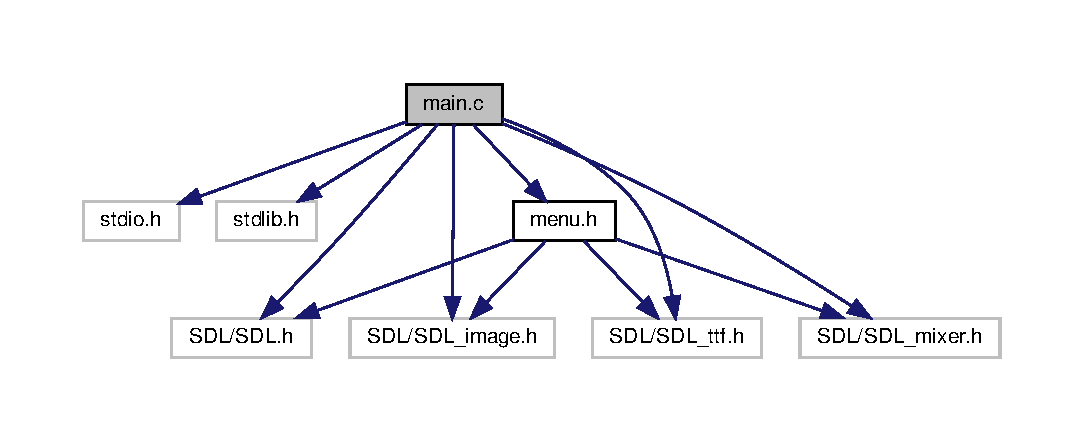
\includegraphics[width=350pt]{main_8c__incl}
\end{center}
\end{figure}
\subsection*{Functions}
\begin{DoxyCompactItemize}
\item 
int \hyperlink{main_8c_ae66f6b31b5ad750f1fe042a706a4e3d4}{main} ()
\end{DoxyCompactItemize}


\subsection{Function Documentation}
\mbox{\Hypertarget{main_8c_ae66f6b31b5ad750f1fe042a706a4e3d4}\label{main_8c_ae66f6b31b5ad750f1fe042a706a4e3d4}} 
\index{main.\+c@{main.\+c}!main@{main}}
\index{main@{main}!main.\+c@{main.\+c}}
\subsubsection{\texorpdfstring{main()}{main()}}
{\footnotesize\ttfamily int main (\begin{DoxyParamCaption}{ }\end{DoxyParamCaption})}

Here is the call graph for this function\+:
\nopagebreak
\begin{figure}[H]
\begin{center}
\leavevmode
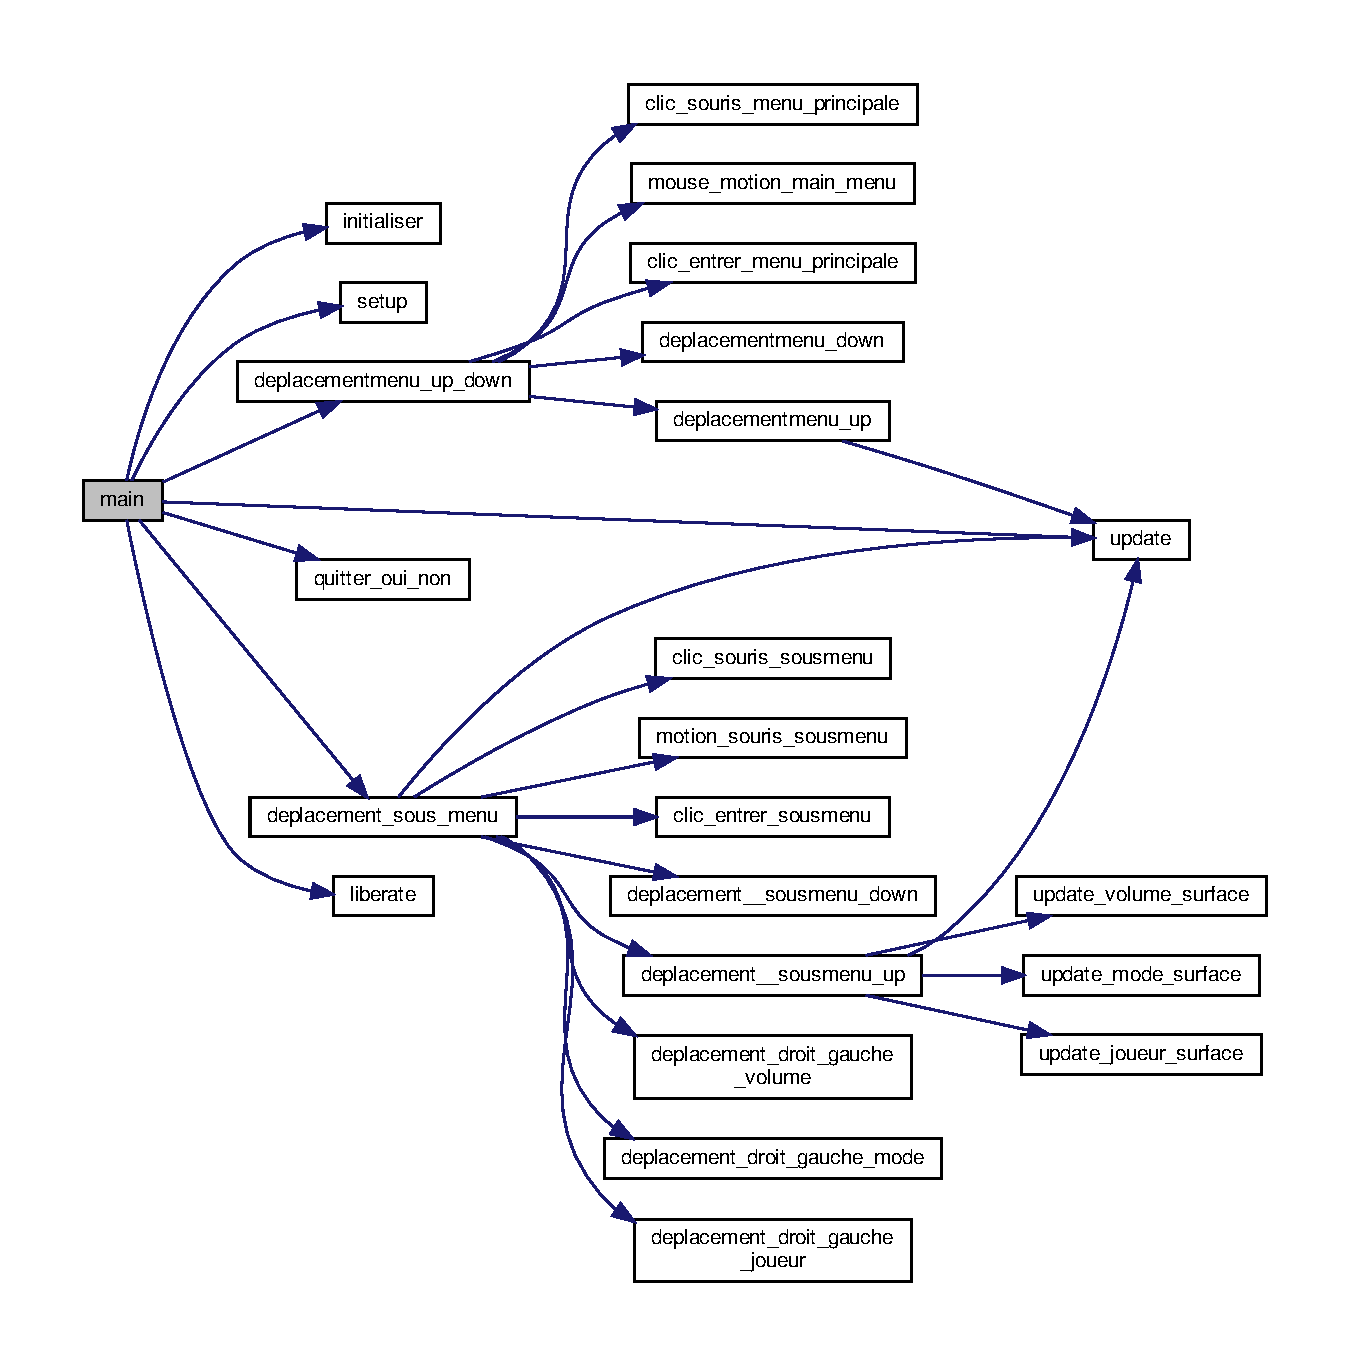
\includegraphics[width=350pt]{main_8c_ae66f6b31b5ad750f1fe042a706a4e3d4_cgraph}
\end{center}
\end{figure}

\hypertarget{menu_01_07copie_08_8c}{}\section{menu (copie).c File Reference}
\label{menu_01_07copie_08_8c}\index{menu (copie).\+c@{menu (copie).\+c}}
{\ttfamily \#include $<$stdio.\+h$>$}\newline
{\ttfamily \#include $<$stdlib.\+h$>$}\newline
{\ttfamily \#include $<$S\+D\+L/\+S\+D\+L.\+h$>$}\newline
{\ttfamily \#include $<$S\+D\+L/\+S\+D\+L\+\_\+image.\+h$>$}\newline
{\ttfamily \#include $<$S\+D\+L/\+S\+D\+L\+\_\+ttf.\+h$>$}\newline
{\ttfamily \#include \char`\"{}S\+D\+L/\+S\+D\+L\+\_\+mixer.\+h\char`\"{}}\newline
{\ttfamily \#include \char`\"{}menu.\+h\char`\"{}}\newline
Include dependency graph for menu (copie).c\+:
\nopagebreak
\begin{figure}[H]
\begin{center}
\leavevmode
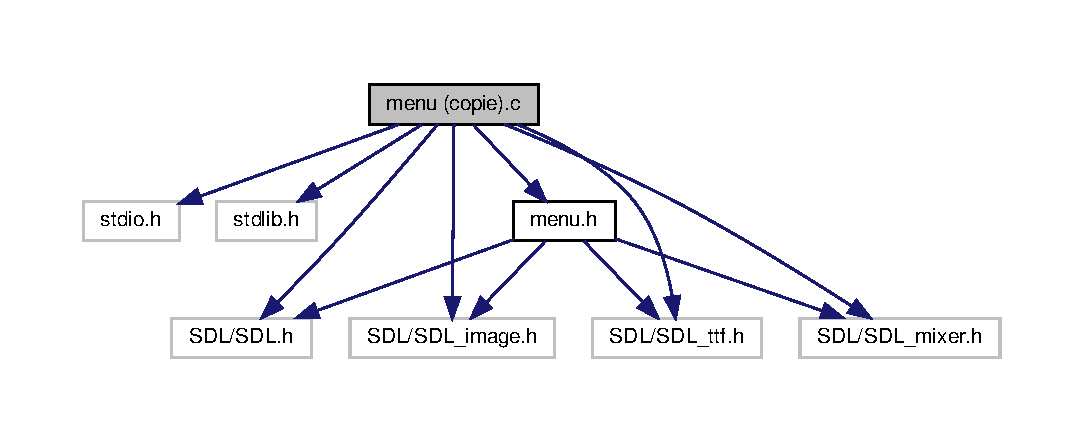
\includegraphics[width=350pt]{menu_01_07copie_08_8c__incl}
\end{center}
\end{figure}
\subsection*{Functions}
\begin{DoxyCompactItemize}
\item 
void \hyperlink{menu_01_07copie_08_8c_a6ed81a9b60090a7e012e1c6a57bbbe57}{initialiser} (\hyperlink{structObjet}{Objet} $\ast$newgame, \hyperlink{structObjet}{Objet} $\ast$loadgame, \hyperlink{structObjet}{Objet} $\ast$settings, \hyperlink{structObjet}{Objet} $\ast$icon, \hyperlink{structObjet}{Objet} $\ast$in\+\_\+sound, \hyperlink{structObjet}{Objet} $\ast$in\+\_\+sound25, \hyperlink{structObjet}{Objet} $\ast$in\+\_\+sound50, \hyperlink{structObjet}{Objet} $\ast$in\+\_\+sound75, \hyperlink{structObjet}{Objet} $\ast$in\+\_\+sound100, \hyperlink{structObjet}{Objet} $\ast$in\+\_\+settings, \hyperlink{structObjet}{Objet} $\ast$credits, \hyperlink{structObjet}{Objet} $\ast$main\+\_\+menu, \hyperlink{structObjet}{Objet} $\ast$quitter, \hyperlink{structObjet}{Objet} $\ast$wexit, \hyperlink{structObjet}{Objet} $\ast$nwexit, \hyperlink{structObjet}{Objet} $\ast$exxit, \hyperlink{structObjet}{Objet} $\ast$game, \hyperlink{structObjet}{Objet} $\ast$j1, \hyperlink{structObjet}{Objet} $\ast$j2, \hyperlink{structObjet}{Objet} $\ast$joueur, \hyperlink{structObjet}{Objet} $\ast$mode, \hyperlink{structObjet}{Objet} $\ast$souris, \hyperlink{structObjet}{Objet} $\ast$clavier, \hyperlink{structObjet}{Objet} $\ast$manette)
\item 
void \hyperlink{menu_01_07copie_08_8c_a74ff2595edb8cb817eeab72f1662171f}{setup} (S\+D\+L\+\_\+\+Surface $\ast$screen, \hyperlink{structObjet}{Objet} $\ast$game, \hyperlink{structObjet}{Objet} $\ast$icon)
\item 
int \hyperlink{menu_01_07copie_08_8c_abe842397d22ae8a423936cc41bba4845}{verif\+\_\+motion\+\_\+surface} (S\+D\+L\+\_\+\+Event event, \hyperlink{structObjet}{Objet} surface)
\item 
void \hyperlink{menu_01_07copie_08_8c_a989655a408019727ed1e4f69cc6cb4e7}{update} (S\+D\+L\+\_\+\+Surface $\ast$screen, \hyperlink{structObjet}{Objet} $\ast$surface1, \hyperlink{structObjet}{Objet} $\ast$surface2)
\item 
void \hyperlink{menu_01_07copie_08_8c_aee999999e7b274237009a249b0227564}{liberate} (\hyperlink{structObjet}{Objet} $\ast$newgame, \hyperlink{structObjet}{Objet} $\ast$loadgame, \hyperlink{structObjet}{Objet} $\ast$settings, \hyperlink{structObjet}{Objet} $\ast$icon, \hyperlink{structObjet}{Objet} $\ast$in\+\_\+sound, \hyperlink{structObjet}{Objet} $\ast$in\+\_\+sound25, \hyperlink{structObjet}{Objet} $\ast$in\+\_\+sound50, \hyperlink{structObjet}{Objet} $\ast$in\+\_\+sound75, \hyperlink{structObjet}{Objet} $\ast$in\+\_\+sound100, \hyperlink{structObjet}{Objet} $\ast$in\+\_\+settings, \hyperlink{structObjet}{Objet} $\ast$credits, \hyperlink{structObjet}{Objet} $\ast$main\+\_\+menu, \hyperlink{structObjet}{Objet} $\ast$quitter, \hyperlink{structObjet}{Objet} $\ast$wexit, \hyperlink{structObjet}{Objet} $\ast$nwexit, \hyperlink{structObjet}{Objet} $\ast$exxit, \hyperlink{structObjet}{Objet} $\ast$game, \hyperlink{structObjet}{Objet} $\ast$j1, \hyperlink{structObjet}{Objet} $\ast$j2, \hyperlink{structObjet}{Objet} $\ast$joueur, \hyperlink{structObjet}{Objet} $\ast$mode, \hyperlink{structObjet}{Objet} $\ast$souris, \hyperlink{structObjet}{Objet} $\ast$clavier, \hyperlink{structObjet}{Objet} $\ast$manette)
\item 
void \hyperlink{menu_01_07copie_08_8c_aa78a832057159b053dc97bc50aaa2f6f}{clic\+\_\+souris\+\_\+menu\+\_\+principale} (S\+D\+L\+\_\+\+Surface $\ast$screen, S\+D\+L\+\_\+\+Event event, int curseur, \hyperlink{structObjet}{Objet} newgame, \hyperlink{structObjet}{Objet} loadgame, \hyperlink{structObjet}{Objet} settings, \hyperlink{structObjet}{Objet} in\+\_\+settings, \hyperlink{structObjet}{Objet} $\ast$icon, \hyperlink{structObjet}{Objet} quitter, int $\ast$in, int $\ast$running, int $\ast$boolean\+\_\+icon, int $\ast$quitt, \hyperlink{structObjet}{Objet} exxit)
\item 
void \hyperlink{menu_01_07copie_08_8c_a5237d05ef4f188f61d5150e4f9ae5114}{clic\+\_\+entrer\+\_\+menu\+\_\+principale} (S\+D\+L\+\_\+\+Surface $\ast$screen, \hyperlink{structObjet}{Objet} in\+\_\+settings, \hyperlink{structObjet}{Objet} icon, Mix\+\_\+\+Chunk $\ast$effect, int curseur, int $\ast$in, int $\ast$running, int $\ast$quitt, \hyperlink{structObjet}{Objet} exxit)
\item 
void \hyperlink{menu_01_07copie_08_8c_a01fee34ecc94975dc64a8b97eec33629}{mouse\+\_\+motion\+\_\+main\+\_\+menu} (S\+D\+L\+\_\+\+Surface $\ast$screen, S\+D\+L\+\_\+\+Event event, Mix\+\_\+\+Chunk $\ast$effect, int $\ast$curseur, \hyperlink{structObjet}{Objet} newgame, \hyperlink{structObjet}{Objet} icon, \hyperlink{structObjet}{Objet} loadgame, \hyperlink{structObjet}{Objet} settings, \hyperlink{structObjet}{Objet} quitter, int $\ast$quitt)
\item 
void \hyperlink{menu_01_07copie_08_8c_aac902a236492a975286b3efad66b5959}{deplacementmenu\+\_\+down} (S\+D\+L\+\_\+\+Surface $\ast$screen, Mix\+\_\+\+Chunk $\ast$effect, int $\ast$curseur, \hyperlink{structObjet}{Objet} newgame, \hyperlink{structObjet}{Objet} icon, \hyperlink{structObjet}{Objet} loadgame, \hyperlink{structObjet}{Objet} settings, \hyperlink{structObjet}{Objet} quitter, int $\ast$quitt)
\item 
void \hyperlink{menu_01_07copie_08_8c_a46a43ec1dbba6ba1beda74652823861c}{deplacementmenu\+\_\+up} (S\+D\+L\+\_\+\+Surface $\ast$screen, Mix\+\_\+\+Chunk $\ast$effect, int $\ast$curseur, \hyperlink{structObjet}{Objet} newgame, \hyperlink{structObjet}{Objet} icon, \hyperlink{structObjet}{Objet} loadgame, \hyperlink{structObjet}{Objet} settings, \hyperlink{structObjet}{Objet} quitter, int $\ast$firsttime, int $\ast$quitt)
\item 
int \hyperlink{menu_01_07copie_08_8c_a8c68826cd41ef1308fa714c9a3932368}{deplacementmenu\+\_\+up\+\_\+down} (S\+D\+L\+\_\+\+Surface $\ast$screen, S\+D\+L\+\_\+\+Event event, int $\ast$firsttime, int $\ast$curseur, int $\ast$running, \hyperlink{structObjet}{Objet} newgame, \hyperlink{structObjet}{Objet} loadgame, \hyperlink{structObjet}{Objet} settings, \hyperlink{structObjet}{Objet} quitter, \hyperlink{structObjet}{Objet} $\ast$icon, \hyperlink{structObjet}{Objet} in\+\_\+settings, Mix\+\_\+\+Chunk $\ast$effect, int $\ast$boolean\+\_\+icon, int $\ast$quitt, \hyperlink{structObjet}{Objet} exxit)
\item 
void \hyperlink{menu_01_07copie_08_8c_a84db6326acd1f67541347734b3a42729}{deplacement\+\_\+\+\_\+sousmenu\+\_\+down} (S\+D\+L\+\_\+\+Surface $\ast$screen, Mix\+\_\+\+Chunk $\ast$effect, int $\ast$curseur, \hyperlink{structObjet}{Objet} in\+\_\+sound, \hyperlink{structObjet}{Objet} in\+\_\+sound25, \hyperlink{structObjet}{Objet} in\+\_\+sound50, \hyperlink{structObjet}{Objet} in\+\_\+sound75, \hyperlink{structObjet}{Objet} in\+\_\+sound100, int position\+\_\+volume, \hyperlink{structObjet}{Objet} icon, \hyperlink{structObjet}{Objet} credits, \hyperlink{structObjet}{Objet} main\+\_\+menu, \hyperlink{structObjet}{Objet} j1, \hyperlink{structObjet}{Objet} j2, \hyperlink{structObjet}{Objet} joueur, \hyperlink{structObjet}{Objet} mode, \hyperlink{structObjet}{Objet} souris, \hyperlink{structObjet}{Objet} clavier, \hyperlink{structObjet}{Objet} manette, int position\+\_\+mode, int position\+\_\+j)
\item 
void \hyperlink{menu_01_07copie_08_8c_aa9aa200c37f08af6f68f5310a3b0f83b}{deplacement\+\_\+\+\_\+sousmenu\+\_\+up} (S\+D\+L\+\_\+\+Surface $\ast$screen, Mix\+\_\+\+Chunk $\ast$effect, int $\ast$curseur, \hyperlink{structObjet}{Objet} in\+\_\+sound, \hyperlink{structObjet}{Objet} in\+\_\+sound25, \hyperlink{structObjet}{Objet} in\+\_\+sound50, \hyperlink{structObjet}{Objet} in\+\_\+sound75, \hyperlink{structObjet}{Objet} in\+\_\+sound100, int position\+\_\+volume, \hyperlink{structObjet}{Objet} icon, \hyperlink{structObjet}{Objet} credits, \hyperlink{structObjet}{Objet} main\+\_\+menu, int $\ast$firsttime, \hyperlink{structObjet}{Objet} j1, \hyperlink{structObjet}{Objet} j2, \hyperlink{structObjet}{Objet} joueur, \hyperlink{structObjet}{Objet} mode, \hyperlink{structObjet}{Objet} souris, \hyperlink{structObjet}{Objet} clavier, \hyperlink{structObjet}{Objet} manette, int position\+\_\+mode, int position\+\_\+j)
\item 
void \hyperlink{menu_01_07copie_08_8c_aafa1723742aaf10400d1226394e81e31}{update\+\_\+volume\+\_\+surface} (S\+D\+L\+\_\+\+Surface $\ast$screen, Mix\+\_\+\+Chunk $\ast$effect, \hyperlink{structObjet}{Objet} in\+\_\+sound, \hyperlink{structObjet}{Objet} in\+\_\+sound25, \hyperlink{structObjet}{Objet} in\+\_\+sound50, \hyperlink{structObjet}{Objet} in\+\_\+sound75, \hyperlink{structObjet}{Objet} in\+\_\+sound100, int position\+\_\+volume)
\item 
void \hyperlink{menu_01_07copie_08_8c_acbff537c998bef21d8aec4663b32500d}{update\+\_\+mode\+\_\+surface} (S\+D\+L\+\_\+\+Surface $\ast$screen, Mix\+\_\+\+Chunk $\ast$effect, \hyperlink{structObjet}{Objet} mode, \hyperlink{structObjet}{Objet} souris, \hyperlink{structObjet}{Objet} clavier, \hyperlink{structObjet}{Objet} manette, int position\+\_\+mode)
\item 
void \hyperlink{menu_01_07copie_08_8c_aacfe086068def17eb2d10ee72c726062}{update\+\_\+joueur\+\_\+surface} (S\+D\+L\+\_\+\+Surface $\ast$screen, Mix\+\_\+\+Chunk $\ast$effect, \hyperlink{structObjet}{Objet} joueur, \hyperlink{structObjet}{Objet} j1, \hyperlink{structObjet}{Objet} j2, int position\+\_\+j)
\item 
void \hyperlink{menu_01_07copie_08_8c_a0ab41f2cf0da8abca3dafab82382517f}{motion\+\_\+souris\+\_\+sousmenu} (S\+D\+L\+\_\+\+Surface $\ast$screen, S\+D\+L\+\_\+\+Event event, Mix\+\_\+\+Chunk $\ast$effect, int $\ast$curseur, \hyperlink{structObjet}{Objet} in\+\_\+sound, \hyperlink{structObjet}{Objet} in\+\_\+sound25, \hyperlink{structObjet}{Objet} in\+\_\+sound50, \hyperlink{structObjet}{Objet} in\+\_\+sound75, \hyperlink{structObjet}{Objet} in\+\_\+sound100, int position\+\_\+volume, \hyperlink{structObjet}{Objet} icon, \hyperlink{structObjet}{Objet} credits, \hyperlink{structObjet}{Objet} main\+\_\+menu, \hyperlink{structObjet}{Objet} j1, \hyperlink{structObjet}{Objet} j2, \hyperlink{structObjet}{Objet} joueur, \hyperlink{structObjet}{Objet} mode, \hyperlink{structObjet}{Objet} souris, \hyperlink{structObjet}{Objet} clavier, \hyperlink{structObjet}{Objet} manette, int position\+\_\+mode, int position\+\_\+j)
\item 
void \hyperlink{menu_01_07copie_08_8c_a7c3b364505423b6ced8dd8ffdb434c13}{clic\+\_\+souris\+\_\+sousmenu} (S\+D\+L\+\_\+\+Surface $\ast$screen, \hyperlink{structObjet}{Objet} $\ast$icon, S\+D\+L\+\_\+\+Event event, int curseur, \hyperlink{structObjet}{Objet} in\+\_\+sound, \hyperlink{structObjet}{Objet} credits, \hyperlink{structObjet}{Objet} main\+\_\+menu, int $\ast$running2, \hyperlink{structObjet}{Objet} game, int $\ast$boolean\+\_\+icon, \hyperlink{structObjet}{Objet} j1, \hyperlink{structObjet}{Objet} j2, \hyperlink{structObjet}{Objet} joueur, \hyperlink{structObjet}{Objet} mode, \hyperlink{structObjet}{Objet} souris, \hyperlink{structObjet}{Objet} clavier, \hyperlink{structObjet}{Objet} manette)
\item 
void \hyperlink{menu_01_07copie_08_8c_ae7c50155f13c09ef789c986059ca3fde}{clic\+\_\+entrer\+\_\+sousmenu} (S\+D\+L\+\_\+\+Surface $\ast$screen, \hyperlink{structObjet}{Objet} icon, int $\ast$running2, int curseur, \hyperlink{structObjet}{Objet} game)
\item 
void \hyperlink{menu_01_07copie_08_8c_a4dda56c63756847abc81ad95418588e9}{deplacement\+\_\+droit\+\_\+gauche\+\_\+volume} (S\+D\+L\+\_\+\+Surface $\ast$screen, Mix\+\_\+\+Chunk $\ast$effect, \hyperlink{structObjet}{Objet} in\+\_\+sound, \hyperlink{structObjet}{Objet} in\+\_\+sound25, \hyperlink{structObjet}{Objet} in\+\_\+sound50, \hyperlink{structObjet}{Objet} in\+\_\+sound75, \hyperlink{structObjet}{Objet} in\+\_\+sound100, int $\ast$position\+\_\+volume)
\item 
void \hyperlink{menu_01_07copie_08_8c_ad913190cb846bda4a0ce88df8871f28b}{deplacement\+\_\+droit\+\_\+gauche\+\_\+mode} (S\+D\+L\+\_\+\+Surface $\ast$screen, Mix\+\_\+\+Chunk $\ast$effect, \hyperlink{structObjet}{Objet} mode, \hyperlink{structObjet}{Objet} souris, \hyperlink{structObjet}{Objet} clavier, \hyperlink{structObjet}{Objet} manette, int $\ast$position\+\_\+mode)
\item 
void \hyperlink{menu_01_07copie_08_8c_ae9a873bbee32be2ae1f56d823111705c}{deplacement\+\_\+droit\+\_\+gauche\+\_\+joueur} (S\+D\+L\+\_\+\+Surface $\ast$screen, Mix\+\_\+\+Chunk $\ast$effect, \hyperlink{structObjet}{Objet} joueur, \hyperlink{structObjet}{Objet} j1, \hyperlink{structObjet}{Objet} j2, int $\ast$position\+\_\+j)
\item 
void \hyperlink{menu_01_07copie_08_8c_a91de672717ace765543b691cc51957f9}{deplacement\+\_\+sous\+\_\+menu} (S\+D\+L\+\_\+\+Surface $\ast$screen, Mix\+\_\+\+Chunk $\ast$effect, S\+D\+L\+\_\+\+Event event, int $\ast$running2, \hyperlink{structObjet}{Objet} in\+\_\+settings, \hyperlink{structObjet}{Objet} in\+\_\+sound, \hyperlink{structObjet}{Objet} in\+\_\+sound25, \hyperlink{structObjet}{Objet} in\+\_\+sound50, \hyperlink{structObjet}{Objet} in\+\_\+sound75, \hyperlink{structObjet}{Objet} in\+\_\+sound100, int $\ast$position\+\_\+volume, \hyperlink{structObjet}{Objet} credits, \hyperlink{structObjet}{Objet} main\+\_\+menu, \hyperlink{structObjet}{Objet} $\ast$icon, int $\ast$running, int $\ast$curseur, int $\ast$firsttime, \hyperlink{structObjet}{Objet} game, int $\ast$boolean\+\_\+icon, \hyperlink{structObjet}{Objet} j1, \hyperlink{structObjet}{Objet} j2, \hyperlink{structObjet}{Objet} joueur, \hyperlink{structObjet}{Objet} mode, \hyperlink{structObjet}{Objet} souris, \hyperlink{structObjet}{Objet} clavier, \hyperlink{structObjet}{Objet} manette, int $\ast$position\+\_\+mode, int $\ast$position\+\_\+j)
\item 
void \hyperlink{menu_01_07copie_08_8c_af4b216a06daa438e8c9d0a41df4d1cd9}{quitter\+\_\+oui\+\_\+non} (S\+D\+L\+\_\+\+Surface $\ast$screen, S\+D\+L\+\_\+\+Event event, int $\ast$running, int $\ast$running2, int $\ast$running3, \hyperlink{structObjet}{Objet} quitter, \hyperlink{structObjet}{Objet} icon, \hyperlink{structObjet}{Objet} wexit, \hyperlink{structObjet}{Objet} nwexit, int $\ast$test, int $\ast$test\+\_\+s)
\end{DoxyCompactItemize}


\subsection{Function Documentation}
\mbox{\Hypertarget{menu_01_07copie_08_8c_a5237d05ef4f188f61d5150e4f9ae5114}\label{menu_01_07copie_08_8c_a5237d05ef4f188f61d5150e4f9ae5114}} 
\index{menu (copie).\+c@{menu (copie).\+c}!clic\+\_\+entrer\+\_\+menu\+\_\+principale@{clic\+\_\+entrer\+\_\+menu\+\_\+principale}}
\index{clic\+\_\+entrer\+\_\+menu\+\_\+principale@{clic\+\_\+entrer\+\_\+menu\+\_\+principale}!menu (copie).\+c@{menu (copie).\+c}}
\subsubsection{\texorpdfstring{clic\+\_\+entrer\+\_\+menu\+\_\+principale()}{clic\_entrer\_menu\_principale()}}
{\footnotesize\ttfamily void clic\+\_\+entrer\+\_\+menu\+\_\+principale (\begin{DoxyParamCaption}\item[{S\+D\+L\+\_\+\+Surface $\ast$}]{screen,  }\item[{\hyperlink{structObjet}{Objet}}]{in\+\_\+settings,  }\item[{\hyperlink{structObjet}{Objet}}]{icon,  }\item[{Mix\+\_\+\+Chunk $\ast$}]{effect,  }\item[{int}]{curseur,  }\item[{int $\ast$}]{in,  }\item[{int $\ast$}]{running,  }\item[{int $\ast$}]{quitt,  }\item[{\hyperlink{structObjet}{Objet}}]{exxit }\end{DoxyParamCaption})}

Here is the caller graph for this function\+:
\nopagebreak
\begin{figure}[H]
\begin{center}
\leavevmode
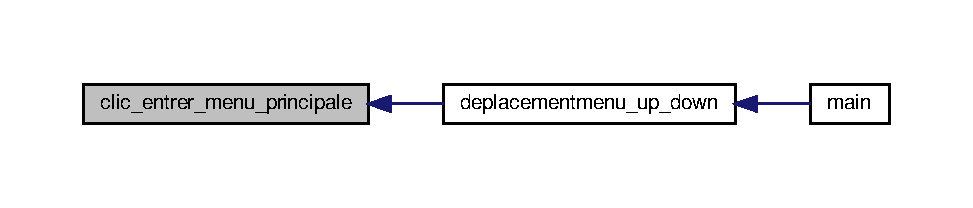
\includegraphics[width=350pt]{menu_01_07copie_08_8c_a5237d05ef4f188f61d5150e4f9ae5114_icgraph}
\end{center}
\end{figure}
\mbox{\Hypertarget{menu_01_07copie_08_8c_ae7c50155f13c09ef789c986059ca3fde}\label{menu_01_07copie_08_8c_ae7c50155f13c09ef789c986059ca3fde}} 
\index{menu (copie).\+c@{menu (copie).\+c}!clic\+\_\+entrer\+\_\+sousmenu@{clic\+\_\+entrer\+\_\+sousmenu}}
\index{clic\+\_\+entrer\+\_\+sousmenu@{clic\+\_\+entrer\+\_\+sousmenu}!menu (copie).\+c@{menu (copie).\+c}}
\subsubsection{\texorpdfstring{clic\+\_\+entrer\+\_\+sousmenu()}{clic\_entrer\_sousmenu()}}
{\footnotesize\ttfamily void clic\+\_\+entrer\+\_\+sousmenu (\begin{DoxyParamCaption}\item[{S\+D\+L\+\_\+\+Surface $\ast$}]{screen,  }\item[{\hyperlink{structObjet}{Objet}}]{icon,  }\item[{int $\ast$}]{running2,  }\item[{int}]{curseur,  }\item[{\hyperlink{structObjet}{Objet}}]{game }\end{DoxyParamCaption})}

Here is the caller graph for this function\+:
\nopagebreak
\begin{figure}[H]
\begin{center}
\leavevmode
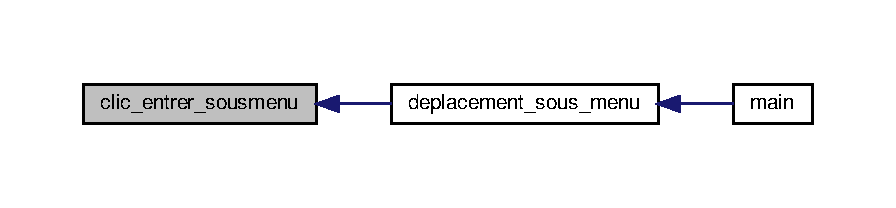
\includegraphics[width=350pt]{menu_01_07copie_08_8c_ae7c50155f13c09ef789c986059ca3fde_icgraph}
\end{center}
\end{figure}
\mbox{\Hypertarget{menu_01_07copie_08_8c_aa78a832057159b053dc97bc50aaa2f6f}\label{menu_01_07copie_08_8c_aa78a832057159b053dc97bc50aaa2f6f}} 
\index{menu (copie).\+c@{menu (copie).\+c}!clic\+\_\+souris\+\_\+menu\+\_\+principale@{clic\+\_\+souris\+\_\+menu\+\_\+principale}}
\index{clic\+\_\+souris\+\_\+menu\+\_\+principale@{clic\+\_\+souris\+\_\+menu\+\_\+principale}!menu (copie).\+c@{menu (copie).\+c}}
\subsubsection{\texorpdfstring{clic\+\_\+souris\+\_\+menu\+\_\+principale()}{clic\_souris\_menu\_principale()}}
{\footnotesize\ttfamily void clic\+\_\+souris\+\_\+menu\+\_\+principale (\begin{DoxyParamCaption}\item[{S\+D\+L\+\_\+\+Surface $\ast$}]{screen,  }\item[{S\+D\+L\+\_\+\+Event}]{event,  }\item[{int}]{curseur,  }\item[{\hyperlink{structObjet}{Objet}}]{newgame,  }\item[{\hyperlink{structObjet}{Objet}}]{loadgame,  }\item[{\hyperlink{structObjet}{Objet}}]{settings,  }\item[{\hyperlink{structObjet}{Objet}}]{in\+\_\+settings,  }\item[{\hyperlink{structObjet}{Objet} $\ast$}]{icon,  }\item[{\hyperlink{structObjet}{Objet}}]{quitter,  }\item[{int $\ast$}]{in,  }\item[{int $\ast$}]{running,  }\item[{int $\ast$}]{boolean\+\_\+icon,  }\item[{int $\ast$}]{quitt,  }\item[{\hyperlink{structObjet}{Objet}}]{exxit }\end{DoxyParamCaption})}

Here is the caller graph for this function\+:
\nopagebreak
\begin{figure}[H]
\begin{center}
\leavevmode
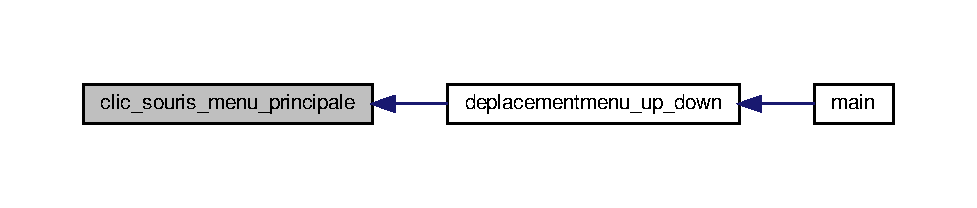
\includegraphics[width=350pt]{menu_01_07copie_08_8c_aa78a832057159b053dc97bc50aaa2f6f_icgraph}
\end{center}
\end{figure}
\mbox{\Hypertarget{menu_01_07copie_08_8c_a7c3b364505423b6ced8dd8ffdb434c13}\label{menu_01_07copie_08_8c_a7c3b364505423b6ced8dd8ffdb434c13}} 
\index{menu (copie).\+c@{menu (copie).\+c}!clic\+\_\+souris\+\_\+sousmenu@{clic\+\_\+souris\+\_\+sousmenu}}
\index{clic\+\_\+souris\+\_\+sousmenu@{clic\+\_\+souris\+\_\+sousmenu}!menu (copie).\+c@{menu (copie).\+c}}
\subsubsection{\texorpdfstring{clic\+\_\+souris\+\_\+sousmenu()}{clic\_souris\_sousmenu()}}
{\footnotesize\ttfamily void clic\+\_\+souris\+\_\+sousmenu (\begin{DoxyParamCaption}\item[{S\+D\+L\+\_\+\+Surface $\ast$}]{screen,  }\item[{\hyperlink{structObjet}{Objet} $\ast$}]{icon,  }\item[{S\+D\+L\+\_\+\+Event}]{event,  }\item[{int}]{curseur,  }\item[{\hyperlink{structObjet}{Objet}}]{in\+\_\+sound,  }\item[{\hyperlink{structObjet}{Objet}}]{credits,  }\item[{\hyperlink{structObjet}{Objet}}]{main\+\_\+menu,  }\item[{int $\ast$}]{running2,  }\item[{\hyperlink{structObjet}{Objet}}]{game,  }\item[{int $\ast$}]{boolean\+\_\+icon,  }\item[{\hyperlink{structObjet}{Objet}}]{j1,  }\item[{\hyperlink{structObjet}{Objet}}]{j2,  }\item[{\hyperlink{structObjet}{Objet}}]{joueur,  }\item[{\hyperlink{structObjet}{Objet}}]{mode,  }\item[{\hyperlink{structObjet}{Objet}}]{souris,  }\item[{\hyperlink{structObjet}{Objet}}]{clavier,  }\item[{\hyperlink{structObjet}{Objet}}]{manette }\end{DoxyParamCaption})}

Here is the caller graph for this function\+:
\nopagebreak
\begin{figure}[H]
\begin{center}
\leavevmode
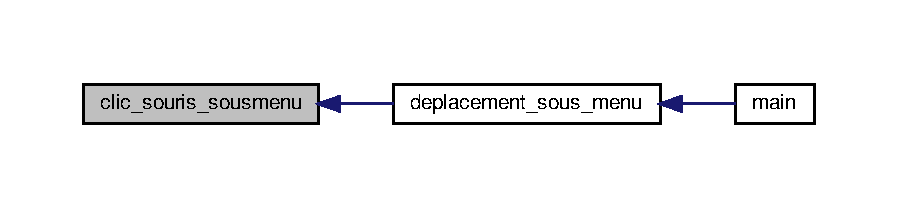
\includegraphics[width=350pt]{menu_01_07copie_08_8c_a7c3b364505423b6ced8dd8ffdb434c13_icgraph}
\end{center}
\end{figure}
\mbox{\Hypertarget{menu_01_07copie_08_8c_a84db6326acd1f67541347734b3a42729}\label{menu_01_07copie_08_8c_a84db6326acd1f67541347734b3a42729}} 
\index{menu (copie).\+c@{menu (copie).\+c}!deplacement\+\_\+\+\_\+sousmenu\+\_\+down@{deplacement\+\_\+\+\_\+sousmenu\+\_\+down}}
\index{deplacement\+\_\+\+\_\+sousmenu\+\_\+down@{deplacement\+\_\+\+\_\+sousmenu\+\_\+down}!menu (copie).\+c@{menu (copie).\+c}}
\subsubsection{\texorpdfstring{deplacement\+\_\+\+\_\+sousmenu\+\_\+down()}{deplacement\_\_sousmenu\_down()}}
{\footnotesize\ttfamily void deplacement\+\_\+\+\_\+sousmenu\+\_\+down (\begin{DoxyParamCaption}\item[{S\+D\+L\+\_\+\+Surface $\ast$}]{screen,  }\item[{Mix\+\_\+\+Chunk $\ast$}]{effect,  }\item[{int $\ast$}]{curseur,  }\item[{\hyperlink{structObjet}{Objet}}]{in\+\_\+sound,  }\item[{\hyperlink{structObjet}{Objet}}]{in\+\_\+sound25,  }\item[{\hyperlink{structObjet}{Objet}}]{in\+\_\+sound50,  }\item[{\hyperlink{structObjet}{Objet}}]{in\+\_\+sound75,  }\item[{\hyperlink{structObjet}{Objet}}]{in\+\_\+sound100,  }\item[{int}]{position\+\_\+volume,  }\item[{\hyperlink{structObjet}{Objet}}]{icon,  }\item[{\hyperlink{structObjet}{Objet}}]{credits,  }\item[{\hyperlink{structObjet}{Objet}}]{main\+\_\+menu,  }\item[{\hyperlink{structObjet}{Objet}}]{j1,  }\item[{\hyperlink{structObjet}{Objet}}]{j2,  }\item[{\hyperlink{structObjet}{Objet}}]{joueur,  }\item[{\hyperlink{structObjet}{Objet}}]{mode,  }\item[{\hyperlink{structObjet}{Objet}}]{souris,  }\item[{\hyperlink{structObjet}{Objet}}]{clavier,  }\item[{\hyperlink{structObjet}{Objet}}]{manette,  }\item[{int}]{position\+\_\+mode,  }\item[{int}]{position\+\_\+j }\end{DoxyParamCaption})}

Here is the caller graph for this function\+:
\nopagebreak
\begin{figure}[H]
\begin{center}
\leavevmode
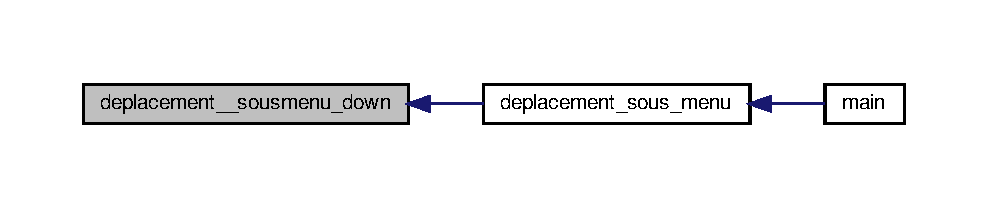
\includegraphics[width=350pt]{menu_01_07copie_08_8c_a84db6326acd1f67541347734b3a42729_icgraph}
\end{center}
\end{figure}
\mbox{\Hypertarget{menu_01_07copie_08_8c_aa9aa200c37f08af6f68f5310a3b0f83b}\label{menu_01_07copie_08_8c_aa9aa200c37f08af6f68f5310a3b0f83b}} 
\index{menu (copie).\+c@{menu (copie).\+c}!deplacement\+\_\+\+\_\+sousmenu\+\_\+up@{deplacement\+\_\+\+\_\+sousmenu\+\_\+up}}
\index{deplacement\+\_\+\+\_\+sousmenu\+\_\+up@{deplacement\+\_\+\+\_\+sousmenu\+\_\+up}!menu (copie).\+c@{menu (copie).\+c}}
\subsubsection{\texorpdfstring{deplacement\+\_\+\+\_\+sousmenu\+\_\+up()}{deplacement\_\_sousmenu\_up()}}
{\footnotesize\ttfamily void deplacement\+\_\+\+\_\+sousmenu\+\_\+up (\begin{DoxyParamCaption}\item[{S\+D\+L\+\_\+\+Surface $\ast$}]{screen,  }\item[{Mix\+\_\+\+Chunk $\ast$}]{effect,  }\item[{int $\ast$}]{curseur,  }\item[{\hyperlink{structObjet}{Objet}}]{in\+\_\+sound,  }\item[{\hyperlink{structObjet}{Objet}}]{in\+\_\+sound25,  }\item[{\hyperlink{structObjet}{Objet}}]{in\+\_\+sound50,  }\item[{\hyperlink{structObjet}{Objet}}]{in\+\_\+sound75,  }\item[{\hyperlink{structObjet}{Objet}}]{in\+\_\+sound100,  }\item[{int}]{position\+\_\+volume,  }\item[{\hyperlink{structObjet}{Objet}}]{icon,  }\item[{\hyperlink{structObjet}{Objet}}]{credits,  }\item[{\hyperlink{structObjet}{Objet}}]{main\+\_\+menu,  }\item[{int $\ast$}]{firsttime,  }\item[{\hyperlink{structObjet}{Objet}}]{j1,  }\item[{\hyperlink{structObjet}{Objet}}]{j2,  }\item[{\hyperlink{structObjet}{Objet}}]{joueur,  }\item[{\hyperlink{structObjet}{Objet}}]{mode,  }\item[{\hyperlink{structObjet}{Objet}}]{souris,  }\item[{\hyperlink{structObjet}{Objet}}]{clavier,  }\item[{\hyperlink{structObjet}{Objet}}]{manette,  }\item[{int}]{position\+\_\+mode,  }\item[{int}]{position\+\_\+j }\end{DoxyParamCaption})}

Here is the call graph for this function\+:
\nopagebreak
\begin{figure}[H]
\begin{center}
\leavevmode
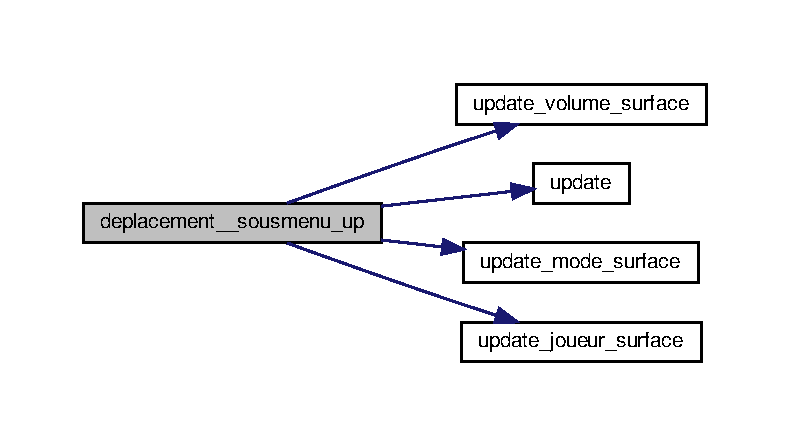
\includegraphics[width=350pt]{menu_01_07copie_08_8c_aa9aa200c37f08af6f68f5310a3b0f83b_cgraph}
\end{center}
\end{figure}
Here is the caller graph for this function\+:
\nopagebreak
\begin{figure}[H]
\begin{center}
\leavevmode
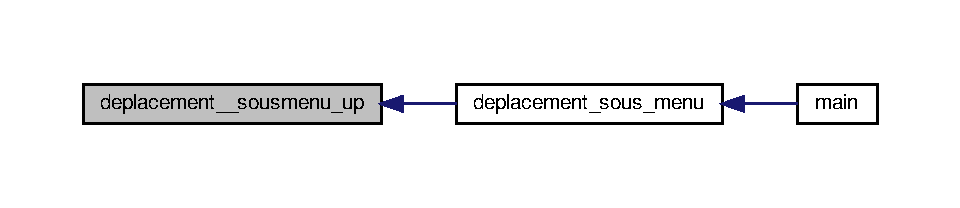
\includegraphics[width=350pt]{menu_01_07copie_08_8c_aa9aa200c37f08af6f68f5310a3b0f83b_icgraph}
\end{center}
\end{figure}
\mbox{\Hypertarget{menu_01_07copie_08_8c_ae9a873bbee32be2ae1f56d823111705c}\label{menu_01_07copie_08_8c_ae9a873bbee32be2ae1f56d823111705c}} 
\index{menu (copie).\+c@{menu (copie).\+c}!deplacement\+\_\+droit\+\_\+gauche\+\_\+joueur@{deplacement\+\_\+droit\+\_\+gauche\+\_\+joueur}}
\index{deplacement\+\_\+droit\+\_\+gauche\+\_\+joueur@{deplacement\+\_\+droit\+\_\+gauche\+\_\+joueur}!menu (copie).\+c@{menu (copie).\+c}}
\subsubsection{\texorpdfstring{deplacement\+\_\+droit\+\_\+gauche\+\_\+joueur()}{deplacement\_droit\_gauche\_joueur()}}
{\footnotesize\ttfamily void deplacement\+\_\+droit\+\_\+gauche\+\_\+joueur (\begin{DoxyParamCaption}\item[{S\+D\+L\+\_\+\+Surface $\ast$}]{screen,  }\item[{Mix\+\_\+\+Chunk $\ast$}]{effect,  }\item[{\hyperlink{structObjet}{Objet}}]{joueur,  }\item[{\hyperlink{structObjet}{Objet}}]{j1,  }\item[{\hyperlink{structObjet}{Objet}}]{j2,  }\item[{int $\ast$}]{position\+\_\+j }\end{DoxyParamCaption})}

Here is the caller graph for this function\+:
\nopagebreak
\begin{figure}[H]
\begin{center}
\leavevmode
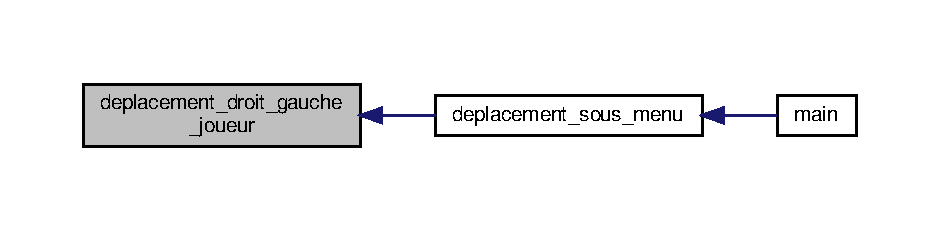
\includegraphics[width=350pt]{menu_01_07copie_08_8c_ae9a873bbee32be2ae1f56d823111705c_icgraph}
\end{center}
\end{figure}
\mbox{\Hypertarget{menu_01_07copie_08_8c_ad913190cb846bda4a0ce88df8871f28b}\label{menu_01_07copie_08_8c_ad913190cb846bda4a0ce88df8871f28b}} 
\index{menu (copie).\+c@{menu (copie).\+c}!deplacement\+\_\+droit\+\_\+gauche\+\_\+mode@{deplacement\+\_\+droit\+\_\+gauche\+\_\+mode}}
\index{deplacement\+\_\+droit\+\_\+gauche\+\_\+mode@{deplacement\+\_\+droit\+\_\+gauche\+\_\+mode}!menu (copie).\+c@{menu (copie).\+c}}
\subsubsection{\texorpdfstring{deplacement\+\_\+droit\+\_\+gauche\+\_\+mode()}{deplacement\_droit\_gauche\_mode()}}
{\footnotesize\ttfamily void deplacement\+\_\+droit\+\_\+gauche\+\_\+mode (\begin{DoxyParamCaption}\item[{S\+D\+L\+\_\+\+Surface $\ast$}]{screen,  }\item[{Mix\+\_\+\+Chunk $\ast$}]{effect,  }\item[{\hyperlink{structObjet}{Objet}}]{mode,  }\item[{\hyperlink{structObjet}{Objet}}]{souris,  }\item[{\hyperlink{structObjet}{Objet}}]{clavier,  }\item[{\hyperlink{structObjet}{Objet}}]{manette,  }\item[{int $\ast$}]{position\+\_\+mode }\end{DoxyParamCaption})}

Here is the caller graph for this function\+:
\nopagebreak
\begin{figure}[H]
\begin{center}
\leavevmode
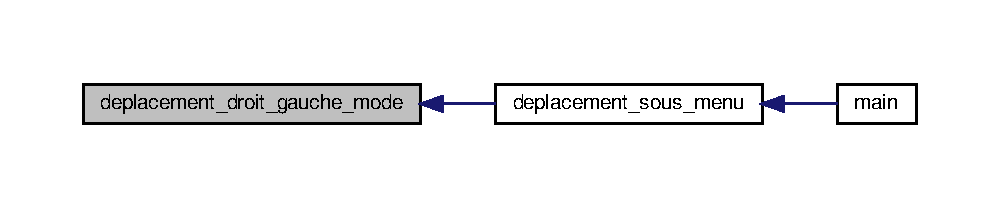
\includegraphics[width=350pt]{menu_01_07copie_08_8c_ad913190cb846bda4a0ce88df8871f28b_icgraph}
\end{center}
\end{figure}
\mbox{\Hypertarget{menu_01_07copie_08_8c_a4dda56c63756847abc81ad95418588e9}\label{menu_01_07copie_08_8c_a4dda56c63756847abc81ad95418588e9}} 
\index{menu (copie).\+c@{menu (copie).\+c}!deplacement\+\_\+droit\+\_\+gauche\+\_\+volume@{deplacement\+\_\+droit\+\_\+gauche\+\_\+volume}}
\index{deplacement\+\_\+droit\+\_\+gauche\+\_\+volume@{deplacement\+\_\+droit\+\_\+gauche\+\_\+volume}!menu (copie).\+c@{menu (copie).\+c}}
\subsubsection{\texorpdfstring{deplacement\+\_\+droit\+\_\+gauche\+\_\+volume()}{deplacement\_droit\_gauche\_volume()}}
{\footnotesize\ttfamily void deplacement\+\_\+droit\+\_\+gauche\+\_\+volume (\begin{DoxyParamCaption}\item[{S\+D\+L\+\_\+\+Surface $\ast$}]{screen,  }\item[{Mix\+\_\+\+Chunk $\ast$}]{effect,  }\item[{\hyperlink{structObjet}{Objet}}]{in\+\_\+sound,  }\item[{\hyperlink{structObjet}{Objet}}]{in\+\_\+sound25,  }\item[{\hyperlink{structObjet}{Objet}}]{in\+\_\+sound50,  }\item[{\hyperlink{structObjet}{Objet}}]{in\+\_\+sound75,  }\item[{\hyperlink{structObjet}{Objet}}]{in\+\_\+sound100,  }\item[{int $\ast$}]{position\+\_\+volume }\end{DoxyParamCaption})}

Here is the caller graph for this function\+:
\nopagebreak
\begin{figure}[H]
\begin{center}
\leavevmode
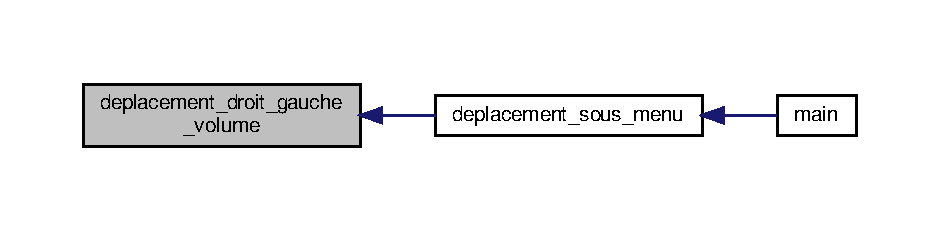
\includegraphics[width=350pt]{menu_01_07copie_08_8c_a4dda56c63756847abc81ad95418588e9_icgraph}
\end{center}
\end{figure}
\mbox{\Hypertarget{menu_01_07copie_08_8c_a91de672717ace765543b691cc51957f9}\label{menu_01_07copie_08_8c_a91de672717ace765543b691cc51957f9}} 
\index{menu (copie).\+c@{menu (copie).\+c}!deplacement\+\_\+sous\+\_\+menu@{deplacement\+\_\+sous\+\_\+menu}}
\index{deplacement\+\_\+sous\+\_\+menu@{deplacement\+\_\+sous\+\_\+menu}!menu (copie).\+c@{menu (copie).\+c}}
\subsubsection{\texorpdfstring{deplacement\+\_\+sous\+\_\+menu()}{deplacement\_sous\_menu()}}
{\footnotesize\ttfamily void deplacement\+\_\+sous\+\_\+menu (\begin{DoxyParamCaption}\item[{S\+D\+L\+\_\+\+Surface $\ast$}]{screen,  }\item[{Mix\+\_\+\+Chunk $\ast$}]{effect,  }\item[{S\+D\+L\+\_\+\+Event}]{event,  }\item[{int $\ast$}]{running2,  }\item[{\hyperlink{structObjet}{Objet}}]{in\+\_\+settings,  }\item[{\hyperlink{structObjet}{Objet}}]{in\+\_\+sound,  }\item[{\hyperlink{structObjet}{Objet}}]{in\+\_\+sound25,  }\item[{\hyperlink{structObjet}{Objet}}]{in\+\_\+sound50,  }\item[{\hyperlink{structObjet}{Objet}}]{in\+\_\+sound75,  }\item[{\hyperlink{structObjet}{Objet}}]{in\+\_\+sound100,  }\item[{int $\ast$}]{position\+\_\+volume,  }\item[{\hyperlink{structObjet}{Objet}}]{credits,  }\item[{\hyperlink{structObjet}{Objet}}]{main\+\_\+menu,  }\item[{\hyperlink{structObjet}{Objet} $\ast$}]{icon,  }\item[{int $\ast$}]{running,  }\item[{int $\ast$}]{curseur,  }\item[{int $\ast$}]{firsttime,  }\item[{\hyperlink{structObjet}{Objet}}]{game,  }\item[{int $\ast$}]{boolean\+\_\+icon,  }\item[{\hyperlink{structObjet}{Objet}}]{j1,  }\item[{\hyperlink{structObjet}{Objet}}]{j2,  }\item[{\hyperlink{structObjet}{Objet}}]{joueur,  }\item[{\hyperlink{structObjet}{Objet}}]{mode,  }\item[{\hyperlink{structObjet}{Objet}}]{souris,  }\item[{\hyperlink{structObjet}{Objet}}]{clavier,  }\item[{\hyperlink{structObjet}{Objet}}]{manette,  }\item[{int $\ast$}]{position\+\_\+mode,  }\item[{int $\ast$}]{position\+\_\+j }\end{DoxyParamCaption})}

Here is the call graph for this function\+:
\nopagebreak
\begin{figure}[H]
\begin{center}
\leavevmode
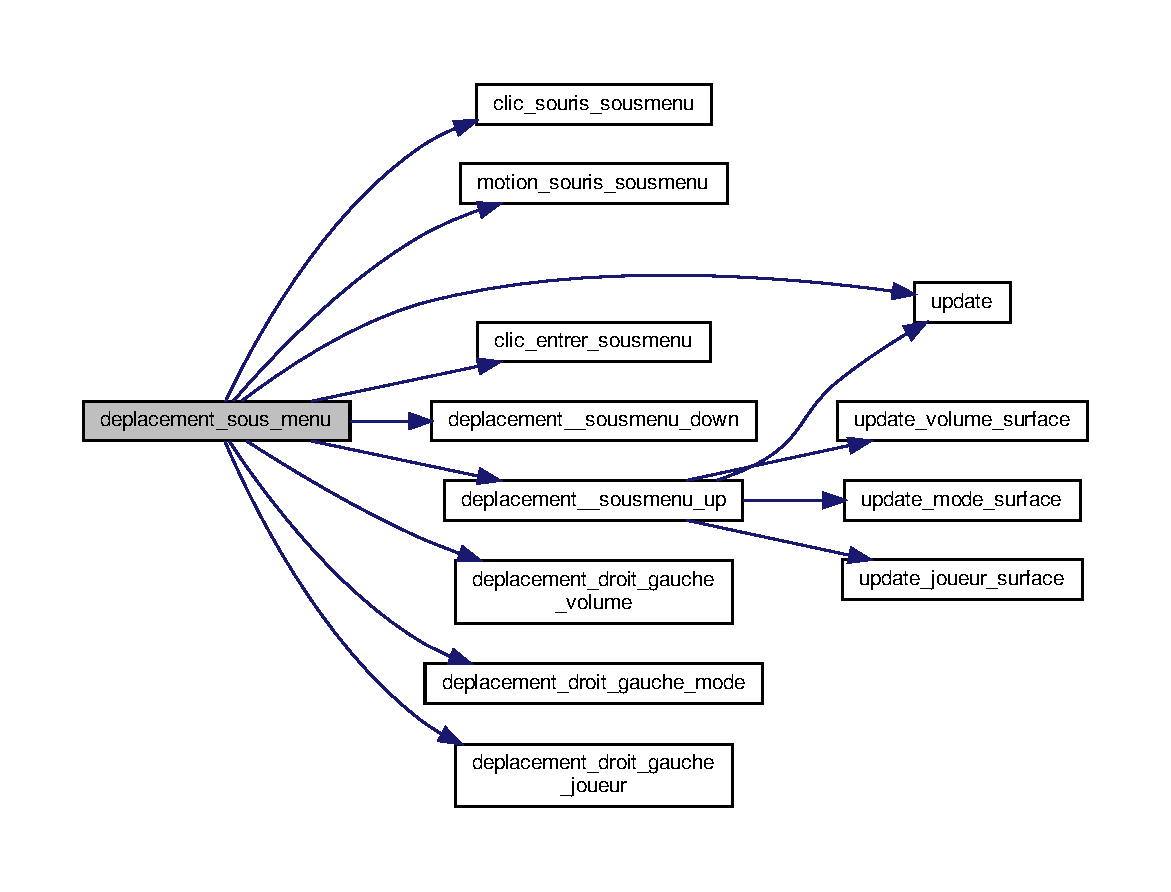
\includegraphics[width=350pt]{menu_01_07copie_08_8c_a91de672717ace765543b691cc51957f9_cgraph}
\end{center}
\end{figure}
Here is the caller graph for this function\+:
\nopagebreak
\begin{figure}[H]
\begin{center}
\leavevmode
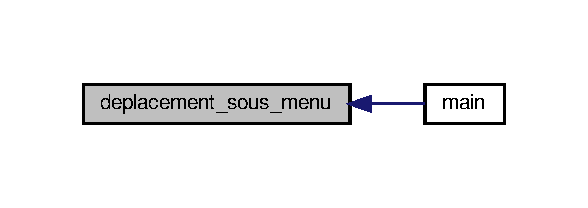
\includegraphics[width=282pt]{menu_01_07copie_08_8c_a91de672717ace765543b691cc51957f9_icgraph}
\end{center}
\end{figure}
\mbox{\Hypertarget{menu_01_07copie_08_8c_aac902a236492a975286b3efad66b5959}\label{menu_01_07copie_08_8c_aac902a236492a975286b3efad66b5959}} 
\index{menu (copie).\+c@{menu (copie).\+c}!deplacementmenu\+\_\+down@{deplacementmenu\+\_\+down}}
\index{deplacementmenu\+\_\+down@{deplacementmenu\+\_\+down}!menu (copie).\+c@{menu (copie).\+c}}
\subsubsection{\texorpdfstring{deplacementmenu\+\_\+down()}{deplacementmenu\_down()}}
{\footnotesize\ttfamily void deplacementmenu\+\_\+down (\begin{DoxyParamCaption}\item[{S\+D\+L\+\_\+\+Surface $\ast$}]{screen,  }\item[{Mix\+\_\+\+Chunk $\ast$}]{effect,  }\item[{int $\ast$}]{curseur,  }\item[{\hyperlink{structObjet}{Objet}}]{newgame,  }\item[{\hyperlink{structObjet}{Objet}}]{icon,  }\item[{\hyperlink{structObjet}{Objet}}]{loadgame,  }\item[{\hyperlink{structObjet}{Objet}}]{settings,  }\item[{\hyperlink{structObjet}{Objet}}]{quitter,  }\item[{int $\ast$}]{quitt }\end{DoxyParamCaption})}

Here is the caller graph for this function\+:
\nopagebreak
\begin{figure}[H]
\begin{center}
\leavevmode
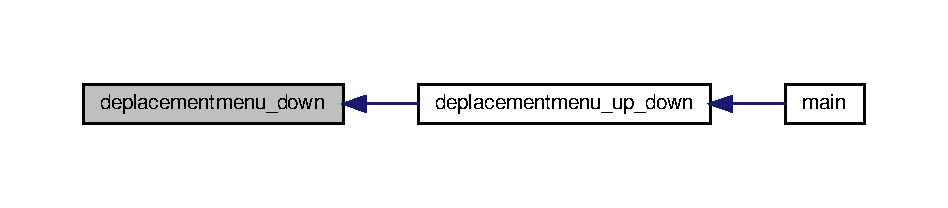
\includegraphics[width=350pt]{menu_01_07copie_08_8c_aac902a236492a975286b3efad66b5959_icgraph}
\end{center}
\end{figure}
\mbox{\Hypertarget{menu_01_07copie_08_8c_a46a43ec1dbba6ba1beda74652823861c}\label{menu_01_07copie_08_8c_a46a43ec1dbba6ba1beda74652823861c}} 
\index{menu (copie).\+c@{menu (copie).\+c}!deplacementmenu\+\_\+up@{deplacementmenu\+\_\+up}}
\index{deplacementmenu\+\_\+up@{deplacementmenu\+\_\+up}!menu (copie).\+c@{menu (copie).\+c}}
\subsubsection{\texorpdfstring{deplacementmenu\+\_\+up()}{deplacementmenu\_up()}}
{\footnotesize\ttfamily void deplacementmenu\+\_\+up (\begin{DoxyParamCaption}\item[{S\+D\+L\+\_\+\+Surface $\ast$}]{screen,  }\item[{Mix\+\_\+\+Chunk $\ast$}]{effect,  }\item[{int $\ast$}]{curseur,  }\item[{\hyperlink{structObjet}{Objet}}]{newgame,  }\item[{\hyperlink{structObjet}{Objet}}]{icon,  }\item[{\hyperlink{structObjet}{Objet}}]{loadgame,  }\item[{\hyperlink{structObjet}{Objet}}]{settings,  }\item[{\hyperlink{structObjet}{Objet}}]{quitter,  }\item[{int $\ast$}]{firsttime,  }\item[{int $\ast$}]{quitt }\end{DoxyParamCaption})}

Here is the call graph for this function\+:
\nopagebreak
\begin{figure}[H]
\begin{center}
\leavevmode
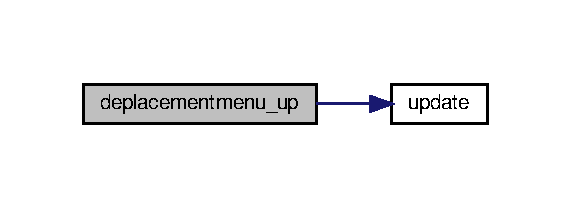
\includegraphics[width=274pt]{menu_01_07copie_08_8c_a46a43ec1dbba6ba1beda74652823861c_cgraph}
\end{center}
\end{figure}
Here is the caller graph for this function\+:
\nopagebreak
\begin{figure}[H]
\begin{center}
\leavevmode
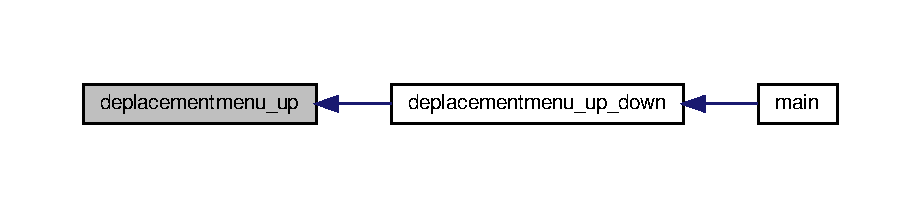
\includegraphics[width=350pt]{menu_01_07copie_08_8c_a46a43ec1dbba6ba1beda74652823861c_icgraph}
\end{center}
\end{figure}
\mbox{\Hypertarget{menu_01_07copie_08_8c_a8c68826cd41ef1308fa714c9a3932368}\label{menu_01_07copie_08_8c_a8c68826cd41ef1308fa714c9a3932368}} 
\index{menu (copie).\+c@{menu (copie).\+c}!deplacementmenu\+\_\+up\+\_\+down@{deplacementmenu\+\_\+up\+\_\+down}}
\index{deplacementmenu\+\_\+up\+\_\+down@{deplacementmenu\+\_\+up\+\_\+down}!menu (copie).\+c@{menu (copie).\+c}}
\subsubsection{\texorpdfstring{deplacementmenu\+\_\+up\+\_\+down()}{deplacementmenu\_up\_down()}}
{\footnotesize\ttfamily int deplacementmenu\+\_\+up\+\_\+down (\begin{DoxyParamCaption}\item[{S\+D\+L\+\_\+\+Surface $\ast$}]{screen,  }\item[{S\+D\+L\+\_\+\+Event}]{event,  }\item[{int $\ast$}]{firsttime,  }\item[{int $\ast$}]{curseur,  }\item[{int $\ast$}]{running,  }\item[{\hyperlink{structObjet}{Objet}}]{newgame,  }\item[{\hyperlink{structObjet}{Objet}}]{loadgame,  }\item[{\hyperlink{structObjet}{Objet}}]{settings,  }\item[{\hyperlink{structObjet}{Objet}}]{quitter,  }\item[{\hyperlink{structObjet}{Objet} $\ast$}]{icon,  }\item[{\hyperlink{structObjet}{Objet}}]{in\+\_\+settings,  }\item[{Mix\+\_\+\+Chunk $\ast$}]{effect,  }\item[{int $\ast$}]{boolean\+\_\+icon,  }\item[{int $\ast$}]{quitt,  }\item[{\hyperlink{structObjet}{Objet}}]{exxit }\end{DoxyParamCaption})}

Here is the call graph for this function\+:
\nopagebreak
\begin{figure}[H]
\begin{center}
\leavevmode
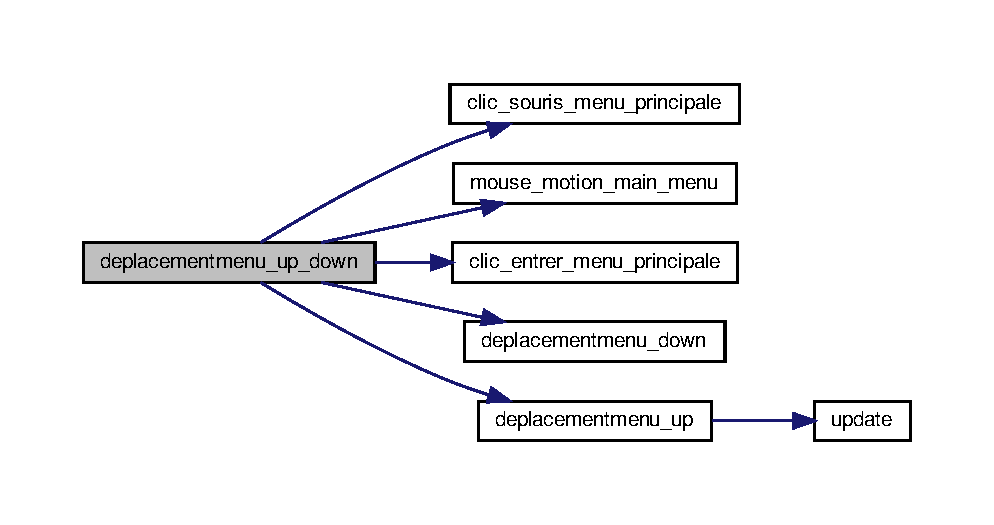
\includegraphics[width=350pt]{menu_01_07copie_08_8c_a8c68826cd41ef1308fa714c9a3932368_cgraph}
\end{center}
\end{figure}
Here is the caller graph for this function\+:
\nopagebreak
\begin{figure}[H]
\begin{center}
\leavevmode
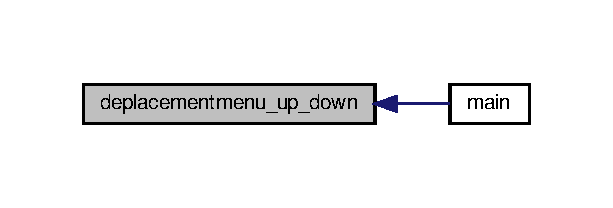
\includegraphics[width=294pt]{menu_01_07copie_08_8c_a8c68826cd41ef1308fa714c9a3932368_icgraph}
\end{center}
\end{figure}
\mbox{\Hypertarget{menu_01_07copie_08_8c_a6ed81a9b60090a7e012e1c6a57bbbe57}\label{menu_01_07copie_08_8c_a6ed81a9b60090a7e012e1c6a57bbbe57}} 
\index{menu (copie).\+c@{menu (copie).\+c}!initialiser@{initialiser}}
\index{initialiser@{initialiser}!menu (copie).\+c@{menu (copie).\+c}}
\subsubsection{\texorpdfstring{initialiser()}{initialiser()}}
{\footnotesize\ttfamily void initialiser (\begin{DoxyParamCaption}\item[{\hyperlink{structObjet}{Objet} $\ast$}]{newgame,  }\item[{\hyperlink{structObjet}{Objet} $\ast$}]{loadgame,  }\item[{\hyperlink{structObjet}{Objet} $\ast$}]{settings,  }\item[{\hyperlink{structObjet}{Objet} $\ast$}]{icon,  }\item[{\hyperlink{structObjet}{Objet} $\ast$}]{in\+\_\+sound,  }\item[{\hyperlink{structObjet}{Objet} $\ast$}]{in\+\_\+sound25,  }\item[{\hyperlink{structObjet}{Objet} $\ast$}]{in\+\_\+sound50,  }\item[{\hyperlink{structObjet}{Objet} $\ast$}]{in\+\_\+sound75,  }\item[{\hyperlink{structObjet}{Objet} $\ast$}]{in\+\_\+sound100,  }\item[{\hyperlink{structObjet}{Objet} $\ast$}]{in\+\_\+settings,  }\item[{\hyperlink{structObjet}{Objet} $\ast$}]{credits,  }\item[{\hyperlink{structObjet}{Objet} $\ast$}]{main\+\_\+menu,  }\item[{\hyperlink{structObjet}{Objet} $\ast$}]{quitter,  }\item[{\hyperlink{structObjet}{Objet} $\ast$}]{wexit,  }\item[{\hyperlink{structObjet}{Objet} $\ast$}]{nwexit,  }\item[{\hyperlink{structObjet}{Objet} $\ast$}]{exxit,  }\item[{\hyperlink{structObjet}{Objet} $\ast$}]{game,  }\item[{\hyperlink{structObjet}{Objet} $\ast$}]{j1,  }\item[{\hyperlink{structObjet}{Objet} $\ast$}]{j2,  }\item[{\hyperlink{structObjet}{Objet} $\ast$}]{joueur,  }\item[{\hyperlink{structObjet}{Objet} $\ast$}]{mode,  }\item[{\hyperlink{structObjet}{Objet} $\ast$}]{souris,  }\item[{\hyperlink{structObjet}{Objet} $\ast$}]{clavier,  }\item[{\hyperlink{structObjet}{Objet} $\ast$}]{manette }\end{DoxyParamCaption})}

Here is the caller graph for this function\+:
\nopagebreak
\begin{figure}[H]
\begin{center}
\leavevmode
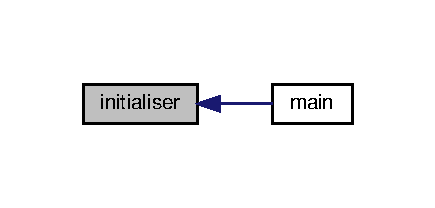
\includegraphics[width=209pt]{menu_01_07copie_08_8c_a6ed81a9b60090a7e012e1c6a57bbbe57_icgraph}
\end{center}
\end{figure}
\mbox{\Hypertarget{menu_01_07copie_08_8c_aee999999e7b274237009a249b0227564}\label{menu_01_07copie_08_8c_aee999999e7b274237009a249b0227564}} 
\index{menu (copie).\+c@{menu (copie).\+c}!liberate@{liberate}}
\index{liberate@{liberate}!menu (copie).\+c@{menu (copie).\+c}}
\subsubsection{\texorpdfstring{liberate()}{liberate()}}
{\footnotesize\ttfamily void liberate (\begin{DoxyParamCaption}\item[{\hyperlink{structObjet}{Objet} $\ast$}]{newgame,  }\item[{\hyperlink{structObjet}{Objet} $\ast$}]{loadgame,  }\item[{\hyperlink{structObjet}{Objet} $\ast$}]{settings,  }\item[{\hyperlink{structObjet}{Objet} $\ast$}]{icon,  }\item[{\hyperlink{structObjet}{Objet} $\ast$}]{in\+\_\+sound,  }\item[{\hyperlink{structObjet}{Objet} $\ast$}]{in\+\_\+sound25,  }\item[{\hyperlink{structObjet}{Objet} $\ast$}]{in\+\_\+sound50,  }\item[{\hyperlink{structObjet}{Objet} $\ast$}]{in\+\_\+sound75,  }\item[{\hyperlink{structObjet}{Objet} $\ast$}]{in\+\_\+sound100,  }\item[{\hyperlink{structObjet}{Objet} $\ast$}]{in\+\_\+settings,  }\item[{\hyperlink{structObjet}{Objet} $\ast$}]{credits,  }\item[{\hyperlink{structObjet}{Objet} $\ast$}]{main\+\_\+menu,  }\item[{\hyperlink{structObjet}{Objet} $\ast$}]{quitter,  }\item[{\hyperlink{structObjet}{Objet} $\ast$}]{wexit,  }\item[{\hyperlink{structObjet}{Objet} $\ast$}]{nwexit,  }\item[{\hyperlink{structObjet}{Objet} $\ast$}]{exxit,  }\item[{\hyperlink{structObjet}{Objet} $\ast$}]{game,  }\item[{\hyperlink{structObjet}{Objet} $\ast$}]{j1,  }\item[{\hyperlink{structObjet}{Objet} $\ast$}]{j2,  }\item[{\hyperlink{structObjet}{Objet} $\ast$}]{joueur,  }\item[{\hyperlink{structObjet}{Objet} $\ast$}]{mode,  }\item[{\hyperlink{structObjet}{Objet} $\ast$}]{souris,  }\item[{\hyperlink{structObjet}{Objet} $\ast$}]{clavier,  }\item[{\hyperlink{structObjet}{Objet} $\ast$}]{manette }\end{DoxyParamCaption})}

Here is the caller graph for this function\+:
\nopagebreak
\begin{figure}[H]
\begin{center}
\leavevmode
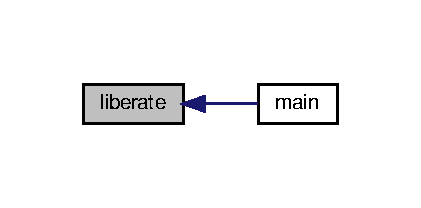
\includegraphics[width=202pt]{menu_01_07copie_08_8c_aee999999e7b274237009a249b0227564_icgraph}
\end{center}
\end{figure}
\mbox{\Hypertarget{menu_01_07copie_08_8c_a0ab41f2cf0da8abca3dafab82382517f}\label{menu_01_07copie_08_8c_a0ab41f2cf0da8abca3dafab82382517f}} 
\index{menu (copie).\+c@{menu (copie).\+c}!motion\+\_\+souris\+\_\+sousmenu@{motion\+\_\+souris\+\_\+sousmenu}}
\index{motion\+\_\+souris\+\_\+sousmenu@{motion\+\_\+souris\+\_\+sousmenu}!menu (copie).\+c@{menu (copie).\+c}}
\subsubsection{\texorpdfstring{motion\+\_\+souris\+\_\+sousmenu()}{motion\_souris\_sousmenu()}}
{\footnotesize\ttfamily void motion\+\_\+souris\+\_\+sousmenu (\begin{DoxyParamCaption}\item[{S\+D\+L\+\_\+\+Surface $\ast$}]{screen,  }\item[{S\+D\+L\+\_\+\+Event}]{event,  }\item[{Mix\+\_\+\+Chunk $\ast$}]{effect,  }\item[{int $\ast$}]{curseur,  }\item[{\hyperlink{structObjet}{Objet}}]{in\+\_\+sound,  }\item[{\hyperlink{structObjet}{Objet}}]{in\+\_\+sound25,  }\item[{\hyperlink{structObjet}{Objet}}]{in\+\_\+sound50,  }\item[{\hyperlink{structObjet}{Objet}}]{in\+\_\+sound75,  }\item[{\hyperlink{structObjet}{Objet}}]{in\+\_\+sound100,  }\item[{int}]{position\+\_\+volume,  }\item[{\hyperlink{structObjet}{Objet}}]{icon,  }\item[{\hyperlink{structObjet}{Objet}}]{credits,  }\item[{\hyperlink{structObjet}{Objet}}]{main\+\_\+menu,  }\item[{\hyperlink{structObjet}{Objet}}]{j1,  }\item[{\hyperlink{structObjet}{Objet}}]{j2,  }\item[{\hyperlink{structObjet}{Objet}}]{joueur,  }\item[{\hyperlink{structObjet}{Objet}}]{mode,  }\item[{\hyperlink{structObjet}{Objet}}]{souris,  }\item[{\hyperlink{structObjet}{Objet}}]{clavier,  }\item[{\hyperlink{structObjet}{Objet}}]{manette,  }\item[{int}]{position\+\_\+mode,  }\item[{int}]{position\+\_\+j }\end{DoxyParamCaption})}

Here is the caller graph for this function\+:
\nopagebreak
\begin{figure}[H]
\begin{center}
\leavevmode
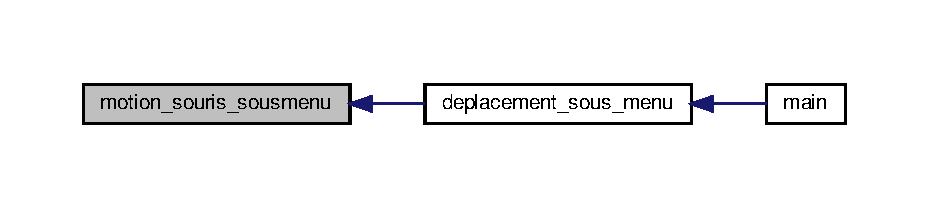
\includegraphics[width=350pt]{menu_01_07copie_08_8c_a0ab41f2cf0da8abca3dafab82382517f_icgraph}
\end{center}
\end{figure}
\mbox{\Hypertarget{menu_01_07copie_08_8c_a01fee34ecc94975dc64a8b97eec33629}\label{menu_01_07copie_08_8c_a01fee34ecc94975dc64a8b97eec33629}} 
\index{menu (copie).\+c@{menu (copie).\+c}!mouse\+\_\+motion\+\_\+main\+\_\+menu@{mouse\+\_\+motion\+\_\+main\+\_\+menu}}
\index{mouse\+\_\+motion\+\_\+main\+\_\+menu@{mouse\+\_\+motion\+\_\+main\+\_\+menu}!menu (copie).\+c@{menu (copie).\+c}}
\subsubsection{\texorpdfstring{mouse\+\_\+motion\+\_\+main\+\_\+menu()}{mouse\_motion\_main\_menu()}}
{\footnotesize\ttfamily void mouse\+\_\+motion\+\_\+main\+\_\+menu (\begin{DoxyParamCaption}\item[{S\+D\+L\+\_\+\+Surface $\ast$}]{screen,  }\item[{S\+D\+L\+\_\+\+Event}]{event,  }\item[{Mix\+\_\+\+Chunk $\ast$}]{effect,  }\item[{int $\ast$}]{curseur,  }\item[{\hyperlink{structObjet}{Objet}}]{newgame,  }\item[{\hyperlink{structObjet}{Objet}}]{icon,  }\item[{\hyperlink{structObjet}{Objet}}]{loadgame,  }\item[{\hyperlink{structObjet}{Objet}}]{settings,  }\item[{\hyperlink{structObjet}{Objet}}]{quitter,  }\item[{int $\ast$}]{quitt }\end{DoxyParamCaption})}

Here is the caller graph for this function\+:
\nopagebreak
\begin{figure}[H]
\begin{center}
\leavevmode
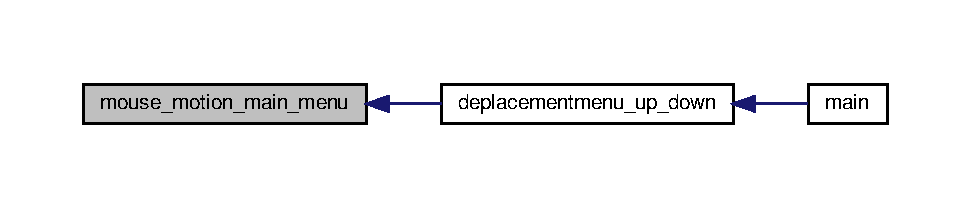
\includegraphics[width=350pt]{menu_01_07copie_08_8c_a01fee34ecc94975dc64a8b97eec33629_icgraph}
\end{center}
\end{figure}
\mbox{\Hypertarget{menu_01_07copie_08_8c_af4b216a06daa438e8c9d0a41df4d1cd9}\label{menu_01_07copie_08_8c_af4b216a06daa438e8c9d0a41df4d1cd9}} 
\index{menu (copie).\+c@{menu (copie).\+c}!quitter\+\_\+oui\+\_\+non@{quitter\+\_\+oui\+\_\+non}}
\index{quitter\+\_\+oui\+\_\+non@{quitter\+\_\+oui\+\_\+non}!menu (copie).\+c@{menu (copie).\+c}}
\subsubsection{\texorpdfstring{quitter\+\_\+oui\+\_\+non()}{quitter\_oui\_non()}}
{\footnotesize\ttfamily void quitter\+\_\+oui\+\_\+non (\begin{DoxyParamCaption}\item[{S\+D\+L\+\_\+\+Surface $\ast$}]{screen,  }\item[{S\+D\+L\+\_\+\+Event}]{event,  }\item[{int $\ast$}]{running,  }\item[{int $\ast$}]{running2,  }\item[{int $\ast$}]{running3,  }\item[{\hyperlink{structObjet}{Objet}}]{quitter,  }\item[{\hyperlink{structObjet}{Objet}}]{icon,  }\item[{\hyperlink{structObjet}{Objet}}]{wexit,  }\item[{\hyperlink{structObjet}{Objet}}]{nwexit,  }\item[{int $\ast$}]{test,  }\item[{int $\ast$}]{test\+\_\+s }\end{DoxyParamCaption})}

Here is the caller graph for this function\+:
\nopagebreak
\begin{figure}[H]
\begin{center}
\leavevmode
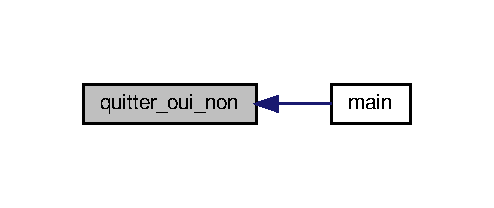
\includegraphics[width=237pt]{menu_01_07copie_08_8c_af4b216a06daa438e8c9d0a41df4d1cd9_icgraph}
\end{center}
\end{figure}
\mbox{\Hypertarget{menu_01_07copie_08_8c_a74ff2595edb8cb817eeab72f1662171f}\label{menu_01_07copie_08_8c_a74ff2595edb8cb817eeab72f1662171f}} 
\index{menu (copie).\+c@{menu (copie).\+c}!setup@{setup}}
\index{setup@{setup}!menu (copie).\+c@{menu (copie).\+c}}
\subsubsection{\texorpdfstring{setup()}{setup()}}
{\footnotesize\ttfamily void setup (\begin{DoxyParamCaption}\item[{S\+D\+L\+\_\+\+Surface $\ast$}]{screen,  }\item[{\hyperlink{structObjet}{Objet} $\ast$}]{game,  }\item[{\hyperlink{structObjet}{Objet} $\ast$}]{icon }\end{DoxyParamCaption})}

Here is the caller graph for this function\+:
\nopagebreak
\begin{figure}[H]
\begin{center}
\leavevmode
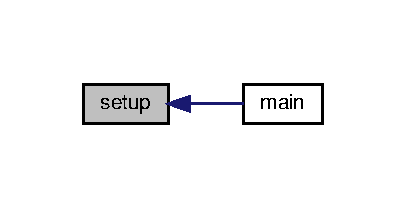
\includegraphics[width=195pt]{menu_01_07copie_08_8c_a74ff2595edb8cb817eeab72f1662171f_icgraph}
\end{center}
\end{figure}
\mbox{\Hypertarget{menu_01_07copie_08_8c_a989655a408019727ed1e4f69cc6cb4e7}\label{menu_01_07copie_08_8c_a989655a408019727ed1e4f69cc6cb4e7}} 
\index{menu (copie).\+c@{menu (copie).\+c}!update@{update}}
\index{update@{update}!menu (copie).\+c@{menu (copie).\+c}}
\subsubsection{\texorpdfstring{update()}{update()}}
{\footnotesize\ttfamily void update (\begin{DoxyParamCaption}\item[{S\+D\+L\+\_\+\+Surface $\ast$}]{screen,  }\item[{\hyperlink{structObjet}{Objet} $\ast$}]{surface1,  }\item[{\hyperlink{structObjet}{Objet} $\ast$}]{surface2 }\end{DoxyParamCaption})}

Here is the caller graph for this function\+:
\nopagebreak
\begin{figure}[H]
\begin{center}
\leavevmode
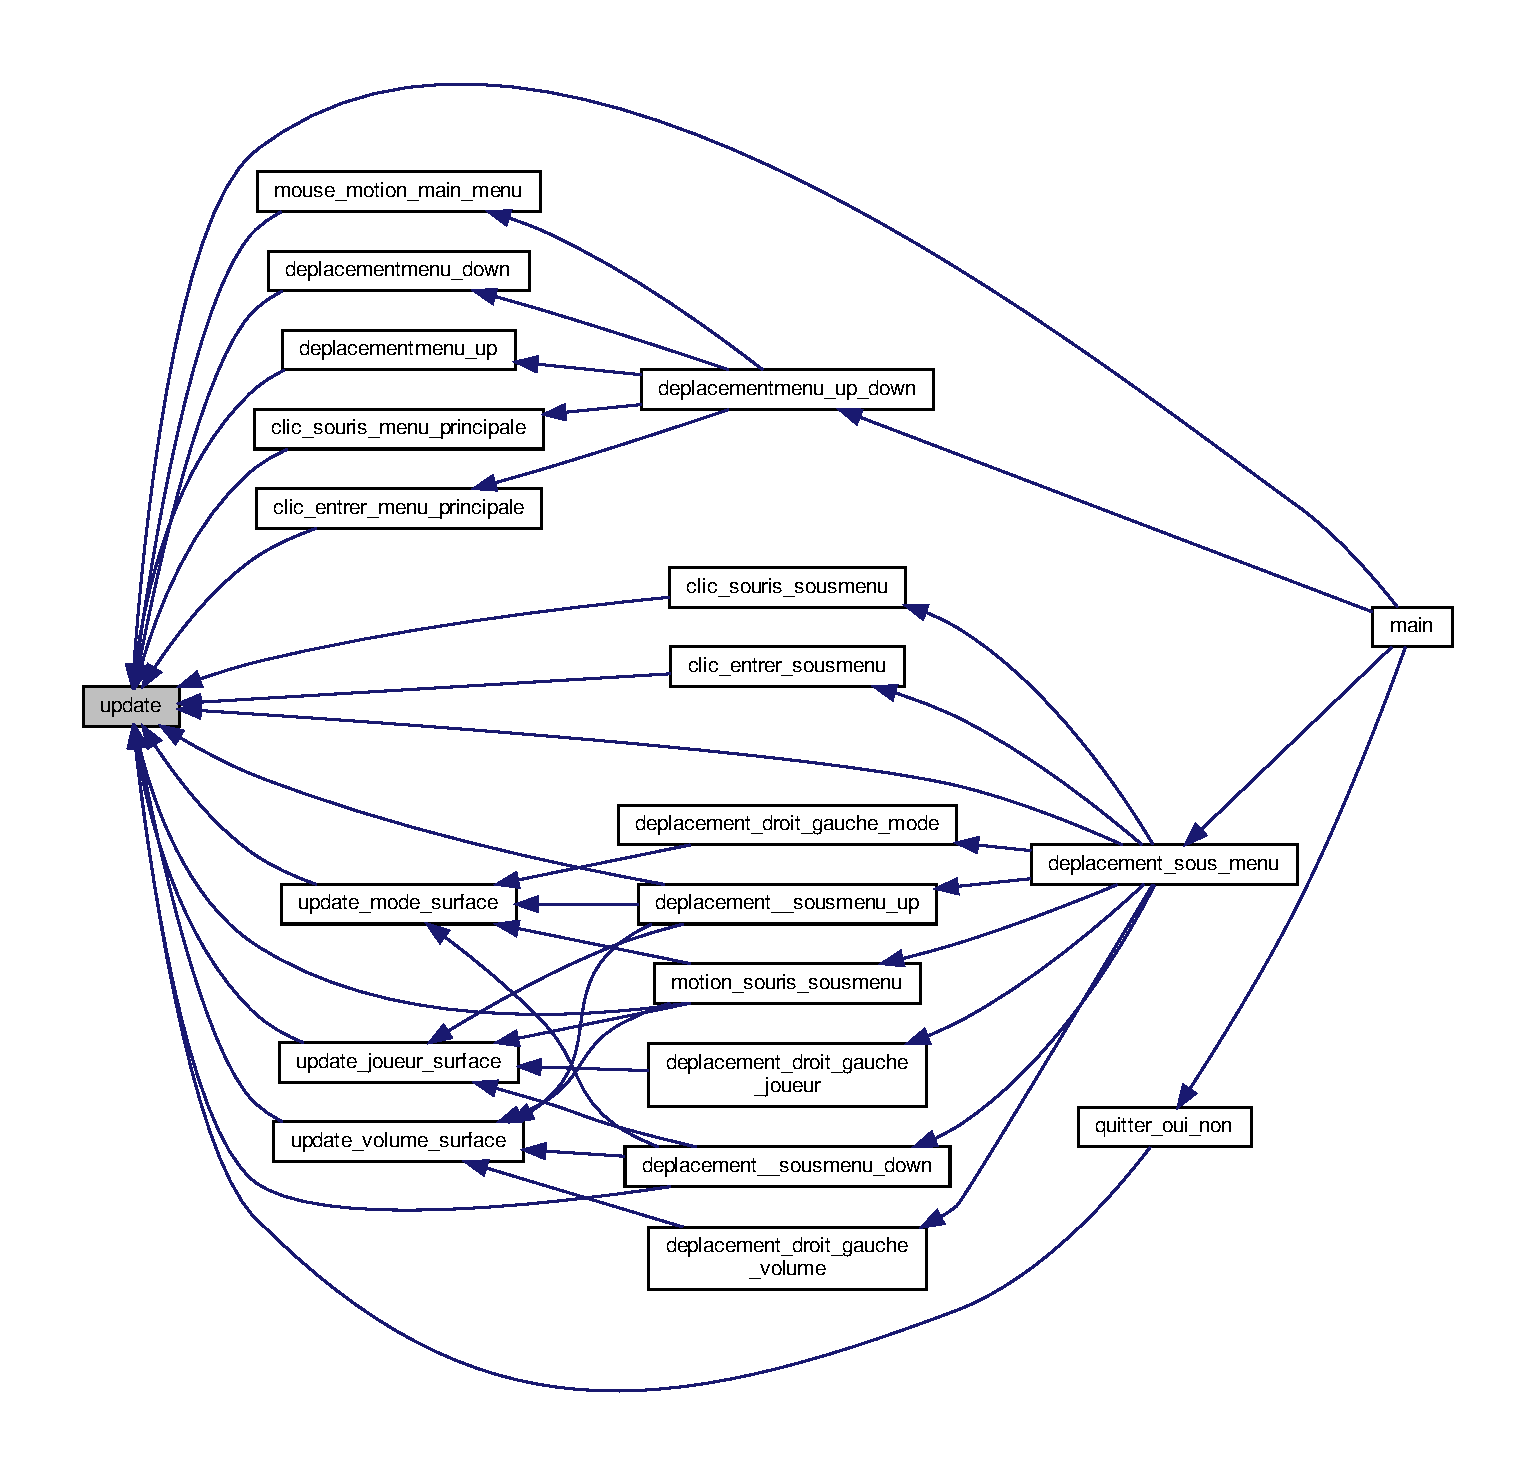
\includegraphics[width=350pt]{menu_01_07copie_08_8c_a989655a408019727ed1e4f69cc6cb4e7_icgraph}
\end{center}
\end{figure}
\mbox{\Hypertarget{menu_01_07copie_08_8c_aacfe086068def17eb2d10ee72c726062}\label{menu_01_07copie_08_8c_aacfe086068def17eb2d10ee72c726062}} 
\index{menu (copie).\+c@{menu (copie).\+c}!update\+\_\+joueur\+\_\+surface@{update\+\_\+joueur\+\_\+surface}}
\index{update\+\_\+joueur\+\_\+surface@{update\+\_\+joueur\+\_\+surface}!menu (copie).\+c@{menu (copie).\+c}}
\subsubsection{\texorpdfstring{update\+\_\+joueur\+\_\+surface()}{update\_joueur\_surface()}}
{\footnotesize\ttfamily void update\+\_\+joueur\+\_\+surface (\begin{DoxyParamCaption}\item[{S\+D\+L\+\_\+\+Surface $\ast$}]{screen,  }\item[{Mix\+\_\+\+Chunk $\ast$}]{effect,  }\item[{\hyperlink{structObjet}{Objet}}]{joueur,  }\item[{\hyperlink{structObjet}{Objet}}]{j1,  }\item[{\hyperlink{structObjet}{Objet}}]{j2,  }\item[{int}]{position\+\_\+j }\end{DoxyParamCaption})}

Here is the caller graph for this function\+:
\nopagebreak
\begin{figure}[H]
\begin{center}
\leavevmode
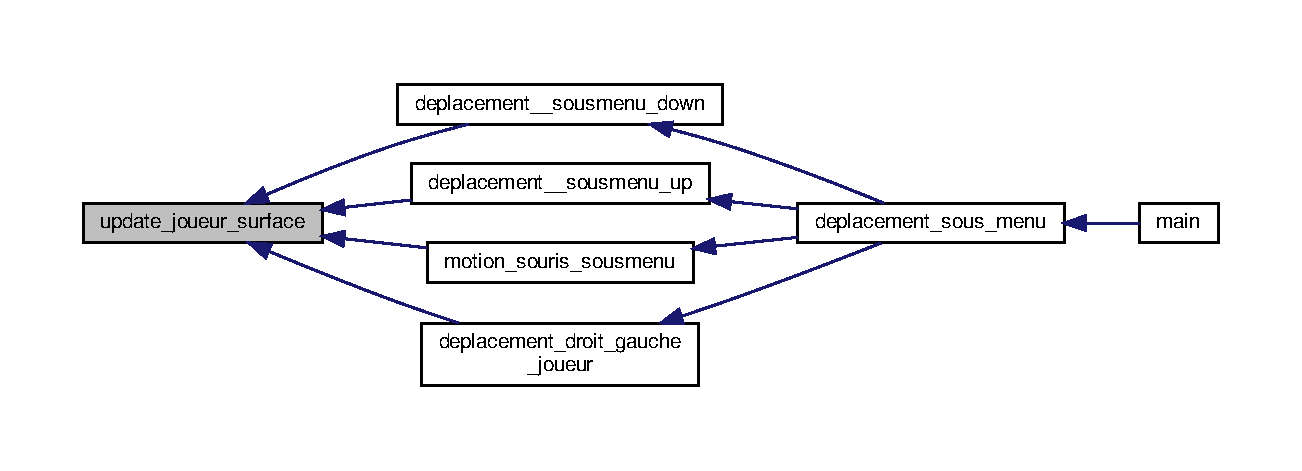
\includegraphics[width=350pt]{menu_01_07copie_08_8c_aacfe086068def17eb2d10ee72c726062_icgraph}
\end{center}
\end{figure}
\mbox{\Hypertarget{menu_01_07copie_08_8c_acbff537c998bef21d8aec4663b32500d}\label{menu_01_07copie_08_8c_acbff537c998bef21d8aec4663b32500d}} 
\index{menu (copie).\+c@{menu (copie).\+c}!update\+\_\+mode\+\_\+surface@{update\+\_\+mode\+\_\+surface}}
\index{update\+\_\+mode\+\_\+surface@{update\+\_\+mode\+\_\+surface}!menu (copie).\+c@{menu (copie).\+c}}
\subsubsection{\texorpdfstring{update\+\_\+mode\+\_\+surface()}{update\_mode\_surface()}}
{\footnotesize\ttfamily void update\+\_\+mode\+\_\+surface (\begin{DoxyParamCaption}\item[{S\+D\+L\+\_\+\+Surface $\ast$}]{screen,  }\item[{Mix\+\_\+\+Chunk $\ast$}]{effect,  }\item[{\hyperlink{structObjet}{Objet}}]{mode,  }\item[{\hyperlink{structObjet}{Objet}}]{souris,  }\item[{\hyperlink{structObjet}{Objet}}]{clavier,  }\item[{\hyperlink{structObjet}{Objet}}]{manette,  }\item[{int}]{position\+\_\+mode }\end{DoxyParamCaption})}

Here is the caller graph for this function\+:
\nopagebreak
\begin{figure}[H]
\begin{center}
\leavevmode
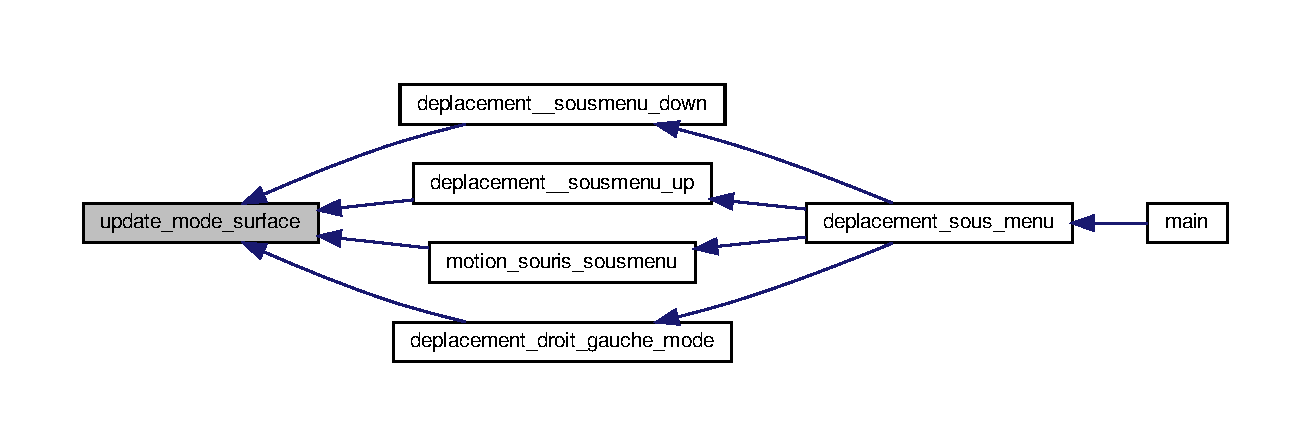
\includegraphics[width=350pt]{menu_01_07copie_08_8c_acbff537c998bef21d8aec4663b32500d_icgraph}
\end{center}
\end{figure}
\mbox{\Hypertarget{menu_01_07copie_08_8c_aafa1723742aaf10400d1226394e81e31}\label{menu_01_07copie_08_8c_aafa1723742aaf10400d1226394e81e31}} 
\index{menu (copie).\+c@{menu (copie).\+c}!update\+\_\+volume\+\_\+surface@{update\+\_\+volume\+\_\+surface}}
\index{update\+\_\+volume\+\_\+surface@{update\+\_\+volume\+\_\+surface}!menu (copie).\+c@{menu (copie).\+c}}
\subsubsection{\texorpdfstring{update\+\_\+volume\+\_\+surface()}{update\_volume\_surface()}}
{\footnotesize\ttfamily void update\+\_\+volume\+\_\+surface (\begin{DoxyParamCaption}\item[{S\+D\+L\+\_\+\+Surface $\ast$}]{screen,  }\item[{Mix\+\_\+\+Chunk $\ast$}]{effect,  }\item[{\hyperlink{structObjet}{Objet}}]{in\+\_\+sound,  }\item[{\hyperlink{structObjet}{Objet}}]{in\+\_\+sound25,  }\item[{\hyperlink{structObjet}{Objet}}]{in\+\_\+sound50,  }\item[{\hyperlink{structObjet}{Objet}}]{in\+\_\+sound75,  }\item[{\hyperlink{structObjet}{Objet}}]{in\+\_\+sound100,  }\item[{int}]{position\+\_\+volume }\end{DoxyParamCaption})}

Here is the caller graph for this function\+:
\nopagebreak
\begin{figure}[H]
\begin{center}
\leavevmode
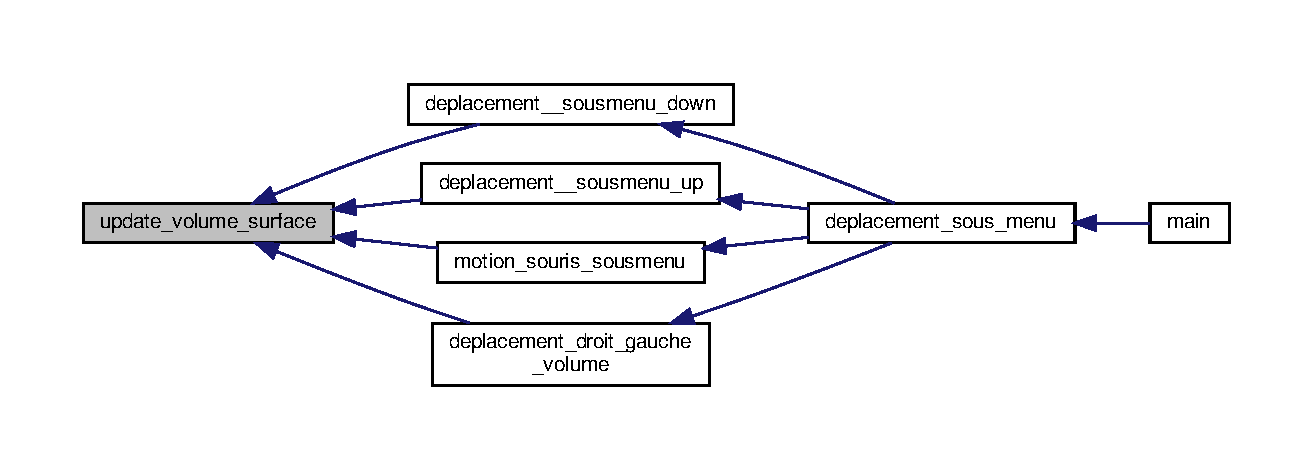
\includegraphics[width=350pt]{menu_01_07copie_08_8c_aafa1723742aaf10400d1226394e81e31_icgraph}
\end{center}
\end{figure}
\mbox{\Hypertarget{menu_01_07copie_08_8c_abe842397d22ae8a423936cc41bba4845}\label{menu_01_07copie_08_8c_abe842397d22ae8a423936cc41bba4845}} 
\index{menu (copie).\+c@{menu (copie).\+c}!verif\+\_\+motion\+\_\+surface@{verif\+\_\+motion\+\_\+surface}}
\index{verif\+\_\+motion\+\_\+surface@{verif\+\_\+motion\+\_\+surface}!menu (copie).\+c@{menu (copie).\+c}}
\subsubsection{\texorpdfstring{verif\+\_\+motion\+\_\+surface()}{verif\_motion\_surface()}}
{\footnotesize\ttfamily int verif\+\_\+motion\+\_\+surface (\begin{DoxyParamCaption}\item[{S\+D\+L\+\_\+\+Event}]{event,  }\item[{\hyperlink{structObjet}{Objet}}]{surface }\end{DoxyParamCaption})}

Here is the caller graph for this function\+:
\nopagebreak
\begin{figure}[H]
\begin{center}
\leavevmode
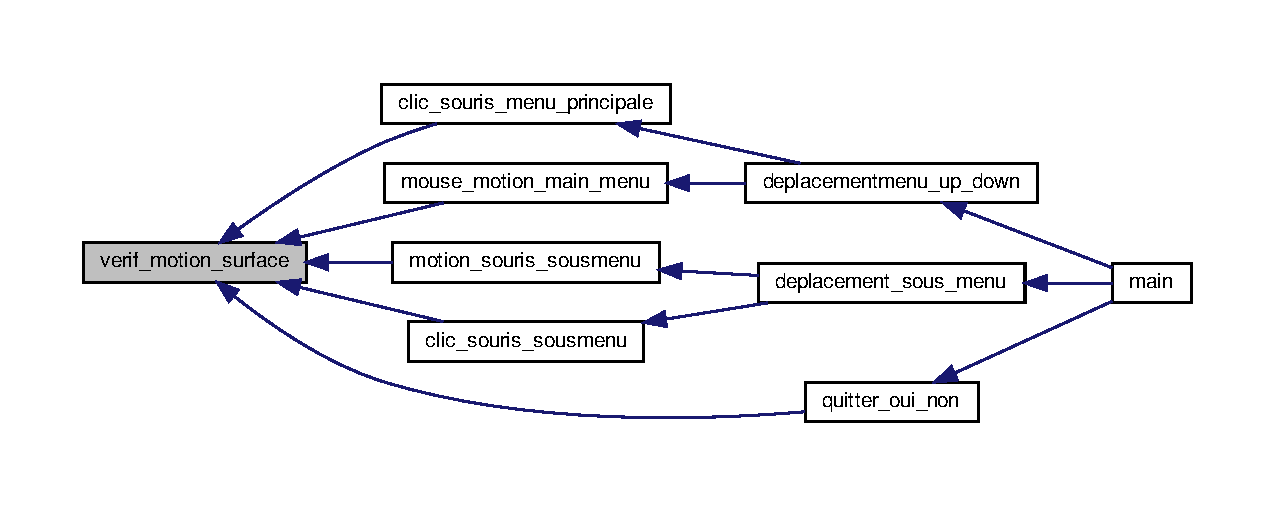
\includegraphics[width=350pt]{menu_01_07copie_08_8c_abe842397d22ae8a423936cc41bba4845_icgraph}
\end{center}
\end{figure}

\hypertarget{menu_8c}{}\section{menu.\+c File Reference}
\label{menu_8c}\index{menu.\+c@{menu.\+c}}
{\ttfamily \#include $<$stdio.\+h$>$}\newline
{\ttfamily \#include $<$stdlib.\+h$>$}\newline
{\ttfamily \#include $<$S\+D\+L/\+S\+D\+L.\+h$>$}\newline
{\ttfamily \#include $<$S\+D\+L/\+S\+D\+L\+\_\+image.\+h$>$}\newline
{\ttfamily \#include $<$S\+D\+L/\+S\+D\+L\+\_\+ttf.\+h$>$}\newline
{\ttfamily \#include \char`\"{}S\+D\+L/\+S\+D\+L\+\_\+mixer.\+h\char`\"{}}\newline
{\ttfamily \#include \char`\"{}menu.\+h\char`\"{}}\newline
Include dependency graph for menu.\+c\+:
\nopagebreak
\begin{figure}[H]
\begin{center}
\leavevmode
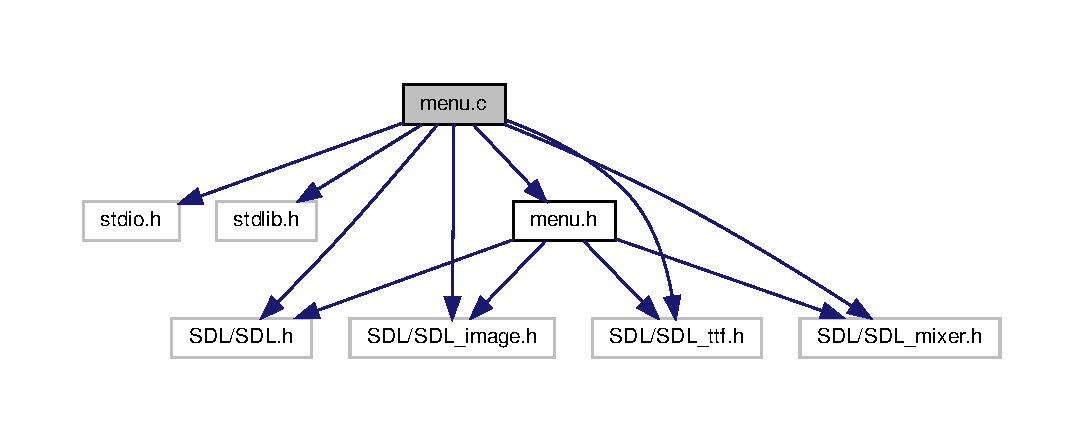
\includegraphics[width=350pt]{menu_8c__incl}
\end{center}
\end{figure}
\subsection*{Functions}
\begin{DoxyCompactItemize}
\item 
void \hyperlink{menu_8c_a6ed81a9b60090a7e012e1c6a57bbbe57}{initialiser} (\hyperlink{structObjet}{Objet} $\ast$newgame, \hyperlink{structObjet}{Objet} $\ast$loadgame, \hyperlink{structObjet}{Objet} $\ast$settings, \hyperlink{structObjet}{Objet} $\ast$icon, \hyperlink{structObjet}{Objet} $\ast$in\+\_\+sound, \hyperlink{structObjet}{Objet} $\ast$in\+\_\+sound25, \hyperlink{structObjet}{Objet} $\ast$in\+\_\+sound50, \hyperlink{structObjet}{Objet} $\ast$in\+\_\+sound75, \hyperlink{structObjet}{Objet} $\ast$in\+\_\+sound100, \hyperlink{structObjet}{Objet} $\ast$in\+\_\+settings, \hyperlink{structObjet}{Objet} $\ast$credits, \hyperlink{structObjet}{Objet} $\ast$main\+\_\+menu, \hyperlink{structObjet}{Objet} $\ast$quitter, \hyperlink{structObjet}{Objet} $\ast$wexit, \hyperlink{structObjet}{Objet} $\ast$nwexit, \hyperlink{structObjet}{Objet} $\ast$exxit, \hyperlink{structObjet}{Objet} $\ast$game, \hyperlink{structObjet}{Objet} $\ast$j1, \hyperlink{structObjet}{Objet} $\ast$j2, \hyperlink{structObjet}{Objet} $\ast$joueur, \hyperlink{structObjet}{Objet} $\ast$mode, \hyperlink{structObjet}{Objet} $\ast$souris, \hyperlink{structObjet}{Objet} $\ast$clavier, \hyperlink{structObjet}{Objet} $\ast$manette)
\item 
void \hyperlink{menu_8c_a74ff2595edb8cb817eeab72f1662171f}{setup} (S\+D\+L\+\_\+\+Surface $\ast$screen, \hyperlink{structObjet}{Objet} $\ast$game, \hyperlink{structObjet}{Objet} $\ast$icon)
\item 
int \hyperlink{menu_8c_abe842397d22ae8a423936cc41bba4845}{verif\+\_\+motion\+\_\+surface} (S\+D\+L\+\_\+\+Event event, \hyperlink{structObjet}{Objet} surface)
\item 
void \hyperlink{menu_8c_a989655a408019727ed1e4f69cc6cb4e7}{update} (S\+D\+L\+\_\+\+Surface $\ast$screen, \hyperlink{structObjet}{Objet} $\ast$surface1, \hyperlink{structObjet}{Objet} $\ast$surface2)
\item 
void \hyperlink{menu_8c_aee999999e7b274237009a249b0227564}{liberate} (\hyperlink{structObjet}{Objet} $\ast$newgame, \hyperlink{structObjet}{Objet} $\ast$loadgame, \hyperlink{structObjet}{Objet} $\ast$settings, \hyperlink{structObjet}{Objet} $\ast$icon, \hyperlink{structObjet}{Objet} $\ast$in\+\_\+sound, \hyperlink{structObjet}{Objet} $\ast$in\+\_\+sound25, \hyperlink{structObjet}{Objet} $\ast$in\+\_\+sound50, \hyperlink{structObjet}{Objet} $\ast$in\+\_\+sound75, \hyperlink{structObjet}{Objet} $\ast$in\+\_\+sound100, \hyperlink{structObjet}{Objet} $\ast$in\+\_\+settings, \hyperlink{structObjet}{Objet} $\ast$credits, \hyperlink{structObjet}{Objet} $\ast$main\+\_\+menu, \hyperlink{structObjet}{Objet} $\ast$quitter, \hyperlink{structObjet}{Objet} $\ast$wexit, \hyperlink{structObjet}{Objet} $\ast$nwexit, \hyperlink{structObjet}{Objet} $\ast$exxit, \hyperlink{structObjet}{Objet} $\ast$game, \hyperlink{structObjet}{Objet} $\ast$j1, \hyperlink{structObjet}{Objet} $\ast$j2, \hyperlink{structObjet}{Objet} $\ast$joueur, \hyperlink{structObjet}{Objet} $\ast$mode, \hyperlink{structObjet}{Objet} $\ast$souris, \hyperlink{structObjet}{Objet} $\ast$clavier, \hyperlink{structObjet}{Objet} $\ast$manette)
\item 
void \hyperlink{menu_8c_aa78a832057159b053dc97bc50aaa2f6f}{clic\+\_\+souris\+\_\+menu\+\_\+principale} (S\+D\+L\+\_\+\+Surface $\ast$screen, S\+D\+L\+\_\+\+Event event, int curseur, \hyperlink{structObjet}{Objet} newgame, \hyperlink{structObjet}{Objet} loadgame, \hyperlink{structObjet}{Objet} settings, \hyperlink{structObjet}{Objet} in\+\_\+settings, \hyperlink{structObjet}{Objet} $\ast$icon, \hyperlink{structObjet}{Objet} quitter, int $\ast$in, int $\ast$running, int $\ast$boolean\+\_\+icon, int $\ast$quitt, \hyperlink{structObjet}{Objet} exxit)
\item 
void \hyperlink{menu_8c_a5237d05ef4f188f61d5150e4f9ae5114}{clic\+\_\+entrer\+\_\+menu\+\_\+principale} (S\+D\+L\+\_\+\+Surface $\ast$screen, \hyperlink{structObjet}{Objet} in\+\_\+settings, \hyperlink{structObjet}{Objet} icon, Mix\+\_\+\+Chunk $\ast$effect, int curseur, int $\ast$in, int $\ast$running, int $\ast$quitt, \hyperlink{structObjet}{Objet} exxit)
\item 
void \hyperlink{menu_8c_a01fee34ecc94975dc64a8b97eec33629}{mouse\+\_\+motion\+\_\+main\+\_\+menu} (S\+D\+L\+\_\+\+Surface $\ast$screen, S\+D\+L\+\_\+\+Event event, Mix\+\_\+\+Chunk $\ast$effect, int $\ast$curseur, \hyperlink{structObjet}{Objet} newgame, \hyperlink{structObjet}{Objet} icon, \hyperlink{structObjet}{Objet} loadgame, \hyperlink{structObjet}{Objet} settings, \hyperlink{structObjet}{Objet} quitter, int $\ast$quitt)
\item 
void \hyperlink{menu_8c_aac902a236492a975286b3efad66b5959}{deplacementmenu\+\_\+down} (S\+D\+L\+\_\+\+Surface $\ast$screen, Mix\+\_\+\+Chunk $\ast$effect, int $\ast$curseur, \hyperlink{structObjet}{Objet} newgame, \hyperlink{structObjet}{Objet} icon, \hyperlink{structObjet}{Objet} loadgame, \hyperlink{structObjet}{Objet} settings, \hyperlink{structObjet}{Objet} quitter, int $\ast$quitt)
\item 
void \hyperlink{menu_8c_aa22c513c93d701f2e2f849693357333e}{deplacementmenu\+\_\+up} (S\+D\+L\+\_\+\+Surface $\ast$screen, Mix\+\_\+\+Chunk $\ast$effect, int $\ast$curseur, \hyperlink{structObjet}{Objet} newgame, \hyperlink{structObjet}{Objet} icon, \hyperlink{structObjet}{Objet} loadgame, \hyperlink{structObjet}{Objet} settings, \hyperlink{structObjet}{Objet} quitter, int $\ast$quitt)
\item 
int \hyperlink{menu_8c_a2268ff186e35842b248248c0c4e8354c}{deplacementmenu\+\_\+up\+\_\+down} (S\+D\+L\+\_\+\+Surface $\ast$screen, S\+D\+L\+\_\+\+Event event, int $\ast$curseur, int $\ast$running, \hyperlink{structObjet}{Objet} newgame, \hyperlink{structObjet}{Objet} loadgame, \hyperlink{structObjet}{Objet} settings, \hyperlink{structObjet}{Objet} quitter, \hyperlink{structObjet}{Objet} $\ast$icon, \hyperlink{structObjet}{Objet} in\+\_\+settings, Mix\+\_\+\+Chunk $\ast$effect, int $\ast$boolean\+\_\+icon, int $\ast$quitt, \hyperlink{structObjet}{Objet} exxit)
\item 
void \hyperlink{menu_8c_a84db6326acd1f67541347734b3a42729}{deplacement\+\_\+\+\_\+sousmenu\+\_\+down} (S\+D\+L\+\_\+\+Surface $\ast$screen, Mix\+\_\+\+Chunk $\ast$effect, int $\ast$curseur, \hyperlink{structObjet}{Objet} in\+\_\+sound, \hyperlink{structObjet}{Objet} in\+\_\+sound25, \hyperlink{structObjet}{Objet} in\+\_\+sound50, \hyperlink{structObjet}{Objet} in\+\_\+sound75, \hyperlink{structObjet}{Objet} in\+\_\+sound100, int position\+\_\+volume, \hyperlink{structObjet}{Objet} icon, \hyperlink{structObjet}{Objet} credits, \hyperlink{structObjet}{Objet} main\+\_\+menu, \hyperlink{structObjet}{Objet} j1, \hyperlink{structObjet}{Objet} j2, \hyperlink{structObjet}{Objet} joueur, \hyperlink{structObjet}{Objet} mode, \hyperlink{structObjet}{Objet} souris, \hyperlink{structObjet}{Objet} clavier, \hyperlink{structObjet}{Objet} manette, int position\+\_\+mode, int position\+\_\+j)
\item 
void \hyperlink{menu_8c_a9e2f67419ed3a0025513ff0f1153b4f0}{deplacement\+\_\+\+\_\+sousmenu\+\_\+up} (S\+D\+L\+\_\+\+Surface $\ast$screen, Mix\+\_\+\+Chunk $\ast$effect, int $\ast$curseur, \hyperlink{structObjet}{Objet} in\+\_\+sound, \hyperlink{structObjet}{Objet} in\+\_\+sound25, \hyperlink{structObjet}{Objet} in\+\_\+sound50, \hyperlink{structObjet}{Objet} in\+\_\+sound75, \hyperlink{structObjet}{Objet} in\+\_\+sound100, int position\+\_\+volume, \hyperlink{structObjet}{Objet} icon, \hyperlink{structObjet}{Objet} credits, \hyperlink{structObjet}{Objet} main\+\_\+menu, \hyperlink{structObjet}{Objet} j1, \hyperlink{structObjet}{Objet} j2, \hyperlink{structObjet}{Objet} joueur, \hyperlink{structObjet}{Objet} mode, \hyperlink{structObjet}{Objet} souris, \hyperlink{structObjet}{Objet} clavier, \hyperlink{structObjet}{Objet} manette, int position\+\_\+mode, int position\+\_\+j)
\item 
void \hyperlink{menu_8c_aafa1723742aaf10400d1226394e81e31}{update\+\_\+volume\+\_\+surface} (S\+D\+L\+\_\+\+Surface $\ast$screen, Mix\+\_\+\+Chunk $\ast$effect, \hyperlink{structObjet}{Objet} in\+\_\+sound, \hyperlink{structObjet}{Objet} in\+\_\+sound25, \hyperlink{structObjet}{Objet} in\+\_\+sound50, \hyperlink{structObjet}{Objet} in\+\_\+sound75, \hyperlink{structObjet}{Objet} in\+\_\+sound100, int position\+\_\+volume)
\item 
void \hyperlink{menu_8c_acbff537c998bef21d8aec4663b32500d}{update\+\_\+mode\+\_\+surface} (S\+D\+L\+\_\+\+Surface $\ast$screen, Mix\+\_\+\+Chunk $\ast$effect, \hyperlink{structObjet}{Objet} mode, \hyperlink{structObjet}{Objet} souris, \hyperlink{structObjet}{Objet} clavier, \hyperlink{structObjet}{Objet} manette, int position\+\_\+mode)
\item 
void \hyperlink{menu_8c_aacfe086068def17eb2d10ee72c726062}{update\+\_\+joueur\+\_\+surface} (S\+D\+L\+\_\+\+Surface $\ast$screen, Mix\+\_\+\+Chunk $\ast$effect, \hyperlink{structObjet}{Objet} joueur, \hyperlink{structObjet}{Objet} j1, \hyperlink{structObjet}{Objet} j2, int position\+\_\+j)
\item 
void \hyperlink{menu_8c_a0ab41f2cf0da8abca3dafab82382517f}{motion\+\_\+souris\+\_\+sousmenu} (S\+D\+L\+\_\+\+Surface $\ast$screen, S\+D\+L\+\_\+\+Event event, Mix\+\_\+\+Chunk $\ast$effect, int $\ast$curseur, \hyperlink{structObjet}{Objet} in\+\_\+sound, \hyperlink{structObjet}{Objet} in\+\_\+sound25, \hyperlink{structObjet}{Objet} in\+\_\+sound50, \hyperlink{structObjet}{Objet} in\+\_\+sound75, \hyperlink{structObjet}{Objet} in\+\_\+sound100, int position\+\_\+volume, \hyperlink{structObjet}{Objet} icon, \hyperlink{structObjet}{Objet} credits, \hyperlink{structObjet}{Objet} main\+\_\+menu, \hyperlink{structObjet}{Objet} j1, \hyperlink{structObjet}{Objet} j2, \hyperlink{structObjet}{Objet} joueur, \hyperlink{structObjet}{Objet} mode, \hyperlink{structObjet}{Objet} souris, \hyperlink{structObjet}{Objet} clavier, \hyperlink{structObjet}{Objet} manette, int position\+\_\+mode, int position\+\_\+j)
\item 
void \hyperlink{menu_8c_a7c3b364505423b6ced8dd8ffdb434c13}{clic\+\_\+souris\+\_\+sousmenu} (S\+D\+L\+\_\+\+Surface $\ast$screen, \hyperlink{structObjet}{Objet} $\ast$icon, S\+D\+L\+\_\+\+Event event, int curseur, \hyperlink{structObjet}{Objet} in\+\_\+sound, \hyperlink{structObjet}{Objet} credits, \hyperlink{structObjet}{Objet} main\+\_\+menu, int $\ast$running2, \hyperlink{structObjet}{Objet} game, int $\ast$boolean\+\_\+icon, \hyperlink{structObjet}{Objet} j1, \hyperlink{structObjet}{Objet} j2, \hyperlink{structObjet}{Objet} joueur, \hyperlink{structObjet}{Objet} mode, \hyperlink{structObjet}{Objet} souris, \hyperlink{structObjet}{Objet} clavier, \hyperlink{structObjet}{Objet} manette)
\item 
void \hyperlink{menu_8c_ae7c50155f13c09ef789c986059ca3fde}{clic\+\_\+entrer\+\_\+sousmenu} (S\+D\+L\+\_\+\+Surface $\ast$screen, \hyperlink{structObjet}{Objet} icon, int $\ast$running2, int curseur, \hyperlink{structObjet}{Objet} game)
\item 
void \hyperlink{menu_8c_a4dda56c63756847abc81ad95418588e9}{deplacement\+\_\+droit\+\_\+gauche\+\_\+volume} (S\+D\+L\+\_\+\+Surface $\ast$screen, Mix\+\_\+\+Chunk $\ast$effect, \hyperlink{structObjet}{Objet} in\+\_\+sound, \hyperlink{structObjet}{Objet} in\+\_\+sound25, \hyperlink{structObjet}{Objet} in\+\_\+sound50, \hyperlink{structObjet}{Objet} in\+\_\+sound75, \hyperlink{structObjet}{Objet} in\+\_\+sound100, int $\ast$position\+\_\+volume)
\item 
void \hyperlink{menu_8c_ad913190cb846bda4a0ce88df8871f28b}{deplacement\+\_\+droit\+\_\+gauche\+\_\+mode} (S\+D\+L\+\_\+\+Surface $\ast$screen, Mix\+\_\+\+Chunk $\ast$effect, \hyperlink{structObjet}{Objet} mode, \hyperlink{structObjet}{Objet} souris, \hyperlink{structObjet}{Objet} clavier, \hyperlink{structObjet}{Objet} manette, int $\ast$position\+\_\+mode)
\item 
void \hyperlink{menu_8c_ae9a873bbee32be2ae1f56d823111705c}{deplacement\+\_\+droit\+\_\+gauche\+\_\+joueur} (S\+D\+L\+\_\+\+Surface $\ast$screen, Mix\+\_\+\+Chunk $\ast$effect, \hyperlink{structObjet}{Objet} joueur, \hyperlink{structObjet}{Objet} j1, \hyperlink{structObjet}{Objet} j2, int $\ast$position\+\_\+j)
\item 
void \hyperlink{menu_8c_a1bc9078394ad9f78ce5a36a6ffcf2f21}{deplacement\+\_\+sous\+\_\+menu} (S\+D\+L\+\_\+\+Surface $\ast$screen, Mix\+\_\+\+Chunk $\ast$effect, S\+D\+L\+\_\+\+Event event, int $\ast$running2, \hyperlink{structObjet}{Objet} in\+\_\+settings, \hyperlink{structObjet}{Objet} in\+\_\+sound, \hyperlink{structObjet}{Objet} in\+\_\+sound25, \hyperlink{structObjet}{Objet} in\+\_\+sound50, \hyperlink{structObjet}{Objet} in\+\_\+sound75, \hyperlink{structObjet}{Objet} in\+\_\+sound100, int $\ast$position\+\_\+volume, \hyperlink{structObjet}{Objet} credits, \hyperlink{structObjet}{Objet} main\+\_\+menu, \hyperlink{structObjet}{Objet} $\ast$icon, int $\ast$running, int $\ast$curseur, \hyperlink{structObjet}{Objet} game, int $\ast$boolean\+\_\+icon, \hyperlink{structObjet}{Objet} j1, \hyperlink{structObjet}{Objet} j2, \hyperlink{structObjet}{Objet} joueur, \hyperlink{structObjet}{Objet} mode, \hyperlink{structObjet}{Objet} souris, \hyperlink{structObjet}{Objet} clavier, \hyperlink{structObjet}{Objet} manette, int $\ast$position\+\_\+mode, int $\ast$position\+\_\+j)
\item 
void \hyperlink{menu_8c_af4b216a06daa438e8c9d0a41df4d1cd9}{quitter\+\_\+oui\+\_\+non} (S\+D\+L\+\_\+\+Surface $\ast$screen, S\+D\+L\+\_\+\+Event event, int $\ast$running, int $\ast$running2, int $\ast$running3, \hyperlink{structObjet}{Objet} quitter, \hyperlink{structObjet}{Objet} icon, \hyperlink{structObjet}{Objet} wexit, \hyperlink{structObjet}{Objet} nwexit, int $\ast$test, int $\ast$test\+\_\+s)
\end{DoxyCompactItemize}


\subsection{Function Documentation}
\mbox{\Hypertarget{menu_8c_a5237d05ef4f188f61d5150e4f9ae5114}\label{menu_8c_a5237d05ef4f188f61d5150e4f9ae5114}} 
\index{menu.\+c@{menu.\+c}!clic\+\_\+entrer\+\_\+menu\+\_\+principale@{clic\+\_\+entrer\+\_\+menu\+\_\+principale}}
\index{clic\+\_\+entrer\+\_\+menu\+\_\+principale@{clic\+\_\+entrer\+\_\+menu\+\_\+principale}!menu.\+c@{menu.\+c}}
\subsubsection{\texorpdfstring{clic\+\_\+entrer\+\_\+menu\+\_\+principale()}{clic\_entrer\_menu\_principale()}}
{\footnotesize\ttfamily void clic\+\_\+entrer\+\_\+menu\+\_\+principale (\begin{DoxyParamCaption}\item[{S\+D\+L\+\_\+\+Surface $\ast$}]{screen,  }\item[{\hyperlink{structObjet}{Objet}}]{in\+\_\+settings,  }\item[{\hyperlink{structObjet}{Objet}}]{icon,  }\item[{Mix\+\_\+\+Chunk $\ast$}]{effect,  }\item[{int}]{curseur,  }\item[{int $\ast$}]{in,  }\item[{int $\ast$}]{running,  }\item[{int $\ast$}]{quitt,  }\item[{\hyperlink{structObjet}{Objet}}]{exxit }\end{DoxyParamCaption})}

Here is the call graph for this function\+:
\nopagebreak
\begin{figure}[H]
\begin{center}
\leavevmode
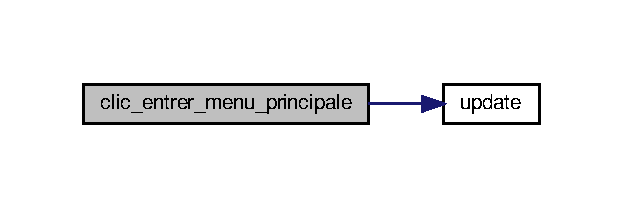
\includegraphics[width=299pt]{menu_8c_a5237d05ef4f188f61d5150e4f9ae5114_cgraph}
\end{center}
\end{figure}
Here is the caller graph for this function\+:
\nopagebreak
\begin{figure}[H]
\begin{center}
\leavevmode
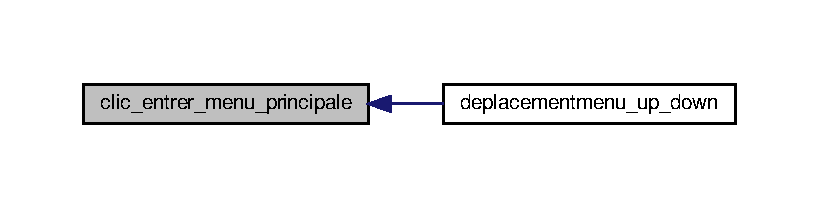
\includegraphics[width=350pt]{menu_8c_a5237d05ef4f188f61d5150e4f9ae5114_icgraph}
\end{center}
\end{figure}
\mbox{\Hypertarget{menu_8c_ae7c50155f13c09ef789c986059ca3fde}\label{menu_8c_ae7c50155f13c09ef789c986059ca3fde}} 
\index{menu.\+c@{menu.\+c}!clic\+\_\+entrer\+\_\+sousmenu@{clic\+\_\+entrer\+\_\+sousmenu}}
\index{clic\+\_\+entrer\+\_\+sousmenu@{clic\+\_\+entrer\+\_\+sousmenu}!menu.\+c@{menu.\+c}}
\subsubsection{\texorpdfstring{clic\+\_\+entrer\+\_\+sousmenu()}{clic\_entrer\_sousmenu()}}
{\footnotesize\ttfamily void clic\+\_\+entrer\+\_\+sousmenu (\begin{DoxyParamCaption}\item[{S\+D\+L\+\_\+\+Surface $\ast$}]{screen,  }\item[{\hyperlink{structObjet}{Objet}}]{icon,  }\item[{int $\ast$}]{running2,  }\item[{int}]{curseur,  }\item[{\hyperlink{structObjet}{Objet}}]{game }\end{DoxyParamCaption})}

Here is the call graph for this function\+:
\nopagebreak
\begin{figure}[H]
\begin{center}
\leavevmode
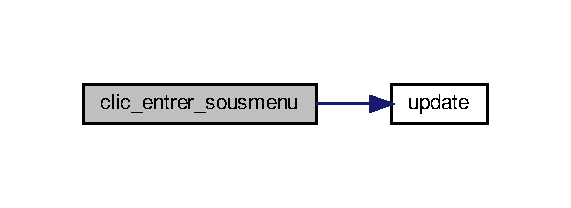
\includegraphics[width=274pt]{menu_8c_ae7c50155f13c09ef789c986059ca3fde_cgraph}
\end{center}
\end{figure}
Here is the caller graph for this function\+:
\nopagebreak
\begin{figure}[H]
\begin{center}
\leavevmode
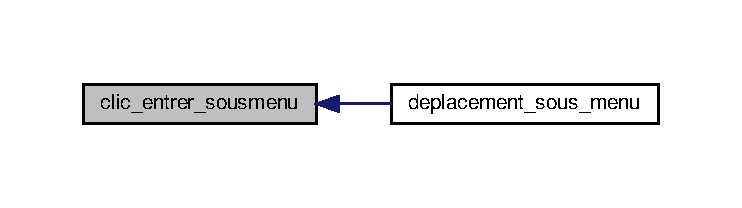
\includegraphics[width=350pt]{menu_8c_ae7c50155f13c09ef789c986059ca3fde_icgraph}
\end{center}
\end{figure}
\mbox{\Hypertarget{menu_8c_aa78a832057159b053dc97bc50aaa2f6f}\label{menu_8c_aa78a832057159b053dc97bc50aaa2f6f}} 
\index{menu.\+c@{menu.\+c}!clic\+\_\+souris\+\_\+menu\+\_\+principale@{clic\+\_\+souris\+\_\+menu\+\_\+principale}}
\index{clic\+\_\+souris\+\_\+menu\+\_\+principale@{clic\+\_\+souris\+\_\+menu\+\_\+principale}!menu.\+c@{menu.\+c}}
\subsubsection{\texorpdfstring{clic\+\_\+souris\+\_\+menu\+\_\+principale()}{clic\_souris\_menu\_principale()}}
{\footnotesize\ttfamily void clic\+\_\+souris\+\_\+menu\+\_\+principale (\begin{DoxyParamCaption}\item[{S\+D\+L\+\_\+\+Surface $\ast$}]{screen,  }\item[{S\+D\+L\+\_\+\+Event}]{event,  }\item[{int}]{curseur,  }\item[{\hyperlink{structObjet}{Objet}}]{newgame,  }\item[{\hyperlink{structObjet}{Objet}}]{loadgame,  }\item[{\hyperlink{structObjet}{Objet}}]{settings,  }\item[{\hyperlink{structObjet}{Objet}}]{in\+\_\+settings,  }\item[{\hyperlink{structObjet}{Objet} $\ast$}]{icon,  }\item[{\hyperlink{structObjet}{Objet}}]{quitter,  }\item[{int $\ast$}]{in,  }\item[{int $\ast$}]{running,  }\item[{int $\ast$}]{boolean\+\_\+icon,  }\item[{int $\ast$}]{quitt,  }\item[{\hyperlink{structObjet}{Objet}}]{exxit }\end{DoxyParamCaption})}

Here is the call graph for this function\+:
\nopagebreak
\begin{figure}[H]
\begin{center}
\leavevmode
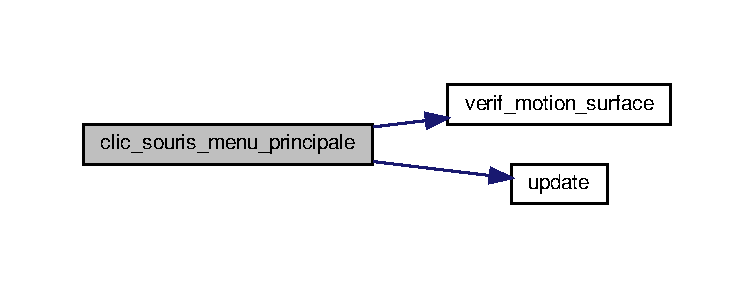
\includegraphics[width=350pt]{menu_8c_aa78a832057159b053dc97bc50aaa2f6f_cgraph}
\end{center}
\end{figure}
Here is the caller graph for this function\+:
\nopagebreak
\begin{figure}[H]
\begin{center}
\leavevmode
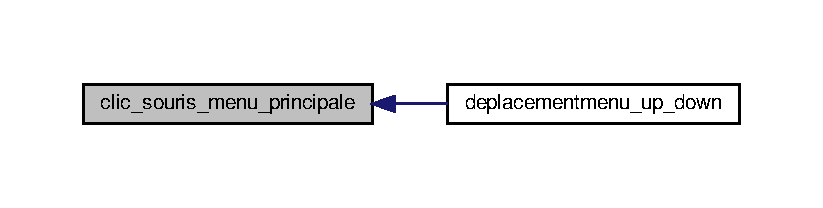
\includegraphics[width=350pt]{menu_8c_aa78a832057159b053dc97bc50aaa2f6f_icgraph}
\end{center}
\end{figure}
\mbox{\Hypertarget{menu_8c_a7c3b364505423b6ced8dd8ffdb434c13}\label{menu_8c_a7c3b364505423b6ced8dd8ffdb434c13}} 
\index{menu.\+c@{menu.\+c}!clic\+\_\+souris\+\_\+sousmenu@{clic\+\_\+souris\+\_\+sousmenu}}
\index{clic\+\_\+souris\+\_\+sousmenu@{clic\+\_\+souris\+\_\+sousmenu}!menu.\+c@{menu.\+c}}
\subsubsection{\texorpdfstring{clic\+\_\+souris\+\_\+sousmenu()}{clic\_souris\_sousmenu()}}
{\footnotesize\ttfamily void clic\+\_\+souris\+\_\+sousmenu (\begin{DoxyParamCaption}\item[{S\+D\+L\+\_\+\+Surface $\ast$}]{screen,  }\item[{\hyperlink{structObjet}{Objet} $\ast$}]{icon,  }\item[{S\+D\+L\+\_\+\+Event}]{event,  }\item[{int}]{curseur,  }\item[{\hyperlink{structObjet}{Objet}}]{in\+\_\+sound,  }\item[{\hyperlink{structObjet}{Objet}}]{credits,  }\item[{\hyperlink{structObjet}{Objet}}]{main\+\_\+menu,  }\item[{int $\ast$}]{running2,  }\item[{\hyperlink{structObjet}{Objet}}]{game,  }\item[{int $\ast$}]{boolean\+\_\+icon,  }\item[{\hyperlink{structObjet}{Objet}}]{j1,  }\item[{\hyperlink{structObjet}{Objet}}]{j2,  }\item[{\hyperlink{structObjet}{Objet}}]{joueur,  }\item[{\hyperlink{structObjet}{Objet}}]{mode,  }\item[{\hyperlink{structObjet}{Objet}}]{souris,  }\item[{\hyperlink{structObjet}{Objet}}]{clavier,  }\item[{\hyperlink{structObjet}{Objet}}]{manette }\end{DoxyParamCaption})}

Here is the call graph for this function\+:
\nopagebreak
\begin{figure}[H]
\begin{center}
\leavevmode
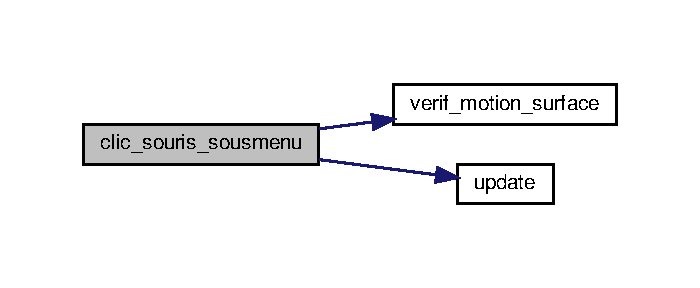
\includegraphics[width=336pt]{menu_8c_a7c3b364505423b6ced8dd8ffdb434c13_cgraph}
\end{center}
\end{figure}
Here is the caller graph for this function\+:
\nopagebreak
\begin{figure}[H]
\begin{center}
\leavevmode
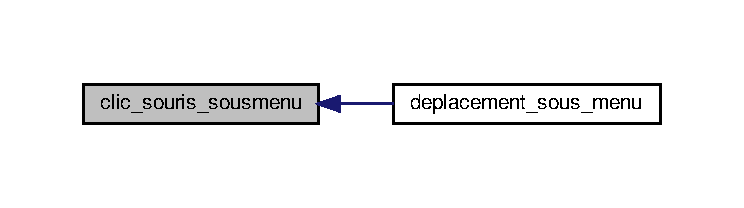
\includegraphics[width=350pt]{menu_8c_a7c3b364505423b6ced8dd8ffdb434c13_icgraph}
\end{center}
\end{figure}
\mbox{\Hypertarget{menu_8c_a84db6326acd1f67541347734b3a42729}\label{menu_8c_a84db6326acd1f67541347734b3a42729}} 
\index{menu.\+c@{menu.\+c}!deplacement\+\_\+\+\_\+sousmenu\+\_\+down@{deplacement\+\_\+\+\_\+sousmenu\+\_\+down}}
\index{deplacement\+\_\+\+\_\+sousmenu\+\_\+down@{deplacement\+\_\+\+\_\+sousmenu\+\_\+down}!menu.\+c@{menu.\+c}}
\subsubsection{\texorpdfstring{deplacement\+\_\+\+\_\+sousmenu\+\_\+down()}{deplacement\_\_sousmenu\_down()}}
{\footnotesize\ttfamily void deplacement\+\_\+\+\_\+sousmenu\+\_\+down (\begin{DoxyParamCaption}\item[{S\+D\+L\+\_\+\+Surface $\ast$}]{screen,  }\item[{Mix\+\_\+\+Chunk $\ast$}]{effect,  }\item[{int $\ast$}]{curseur,  }\item[{\hyperlink{structObjet}{Objet}}]{in\+\_\+sound,  }\item[{\hyperlink{structObjet}{Objet}}]{in\+\_\+sound25,  }\item[{\hyperlink{structObjet}{Objet}}]{in\+\_\+sound50,  }\item[{\hyperlink{structObjet}{Objet}}]{in\+\_\+sound75,  }\item[{\hyperlink{structObjet}{Objet}}]{in\+\_\+sound100,  }\item[{int}]{position\+\_\+volume,  }\item[{\hyperlink{structObjet}{Objet}}]{icon,  }\item[{\hyperlink{structObjet}{Objet}}]{credits,  }\item[{\hyperlink{structObjet}{Objet}}]{main\+\_\+menu,  }\item[{\hyperlink{structObjet}{Objet}}]{j1,  }\item[{\hyperlink{structObjet}{Objet}}]{j2,  }\item[{\hyperlink{structObjet}{Objet}}]{joueur,  }\item[{\hyperlink{structObjet}{Objet}}]{mode,  }\item[{\hyperlink{structObjet}{Objet}}]{souris,  }\item[{\hyperlink{structObjet}{Objet}}]{clavier,  }\item[{\hyperlink{structObjet}{Objet}}]{manette,  }\item[{int}]{position\+\_\+mode,  }\item[{int}]{position\+\_\+j }\end{DoxyParamCaption})}

Here is the call graph for this function\+:
\nopagebreak
\begin{figure}[H]
\begin{center}
\leavevmode
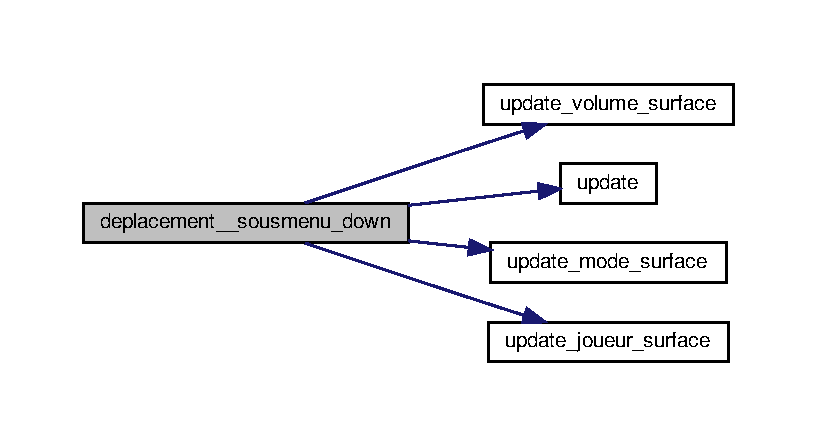
\includegraphics[width=350pt]{menu_8c_a84db6326acd1f67541347734b3a42729_cgraph}
\end{center}
\end{figure}
Here is the caller graph for this function\+:
\nopagebreak
\begin{figure}[H]
\begin{center}
\leavevmode
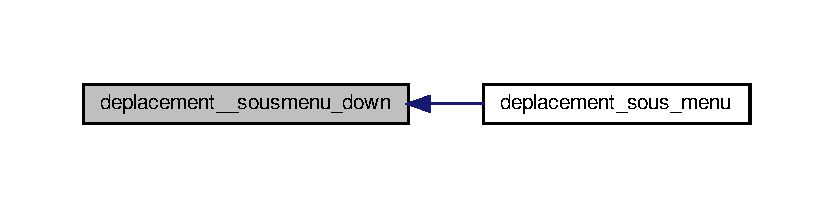
\includegraphics[width=350pt]{menu_8c_a84db6326acd1f67541347734b3a42729_icgraph}
\end{center}
\end{figure}
\mbox{\Hypertarget{menu_8c_a9e2f67419ed3a0025513ff0f1153b4f0}\label{menu_8c_a9e2f67419ed3a0025513ff0f1153b4f0}} 
\index{menu.\+c@{menu.\+c}!deplacement\+\_\+\+\_\+sousmenu\+\_\+up@{deplacement\+\_\+\+\_\+sousmenu\+\_\+up}}
\index{deplacement\+\_\+\+\_\+sousmenu\+\_\+up@{deplacement\+\_\+\+\_\+sousmenu\+\_\+up}!menu.\+c@{menu.\+c}}
\subsubsection{\texorpdfstring{deplacement\+\_\+\+\_\+sousmenu\+\_\+up()}{deplacement\_\_sousmenu\_up()}}
{\footnotesize\ttfamily void deplacement\+\_\+\+\_\+sousmenu\+\_\+up (\begin{DoxyParamCaption}\item[{S\+D\+L\+\_\+\+Surface $\ast$}]{screen,  }\item[{Mix\+\_\+\+Chunk $\ast$}]{effect,  }\item[{int $\ast$}]{curseur,  }\item[{\hyperlink{structObjet}{Objet}}]{in\+\_\+sound,  }\item[{\hyperlink{structObjet}{Objet}}]{in\+\_\+sound25,  }\item[{\hyperlink{structObjet}{Objet}}]{in\+\_\+sound50,  }\item[{\hyperlink{structObjet}{Objet}}]{in\+\_\+sound75,  }\item[{\hyperlink{structObjet}{Objet}}]{in\+\_\+sound100,  }\item[{int}]{position\+\_\+volume,  }\item[{\hyperlink{structObjet}{Objet}}]{icon,  }\item[{\hyperlink{structObjet}{Objet}}]{credits,  }\item[{\hyperlink{structObjet}{Objet}}]{main\+\_\+menu,  }\item[{\hyperlink{structObjet}{Objet}}]{j1,  }\item[{\hyperlink{structObjet}{Objet}}]{j2,  }\item[{\hyperlink{structObjet}{Objet}}]{joueur,  }\item[{\hyperlink{structObjet}{Objet}}]{mode,  }\item[{\hyperlink{structObjet}{Objet}}]{souris,  }\item[{\hyperlink{structObjet}{Objet}}]{clavier,  }\item[{\hyperlink{structObjet}{Objet}}]{manette,  }\item[{int}]{position\+\_\+mode,  }\item[{int}]{position\+\_\+j }\end{DoxyParamCaption})}

Here is the call graph for this function\+:
\nopagebreak
\begin{figure}[H]
\begin{center}
\leavevmode
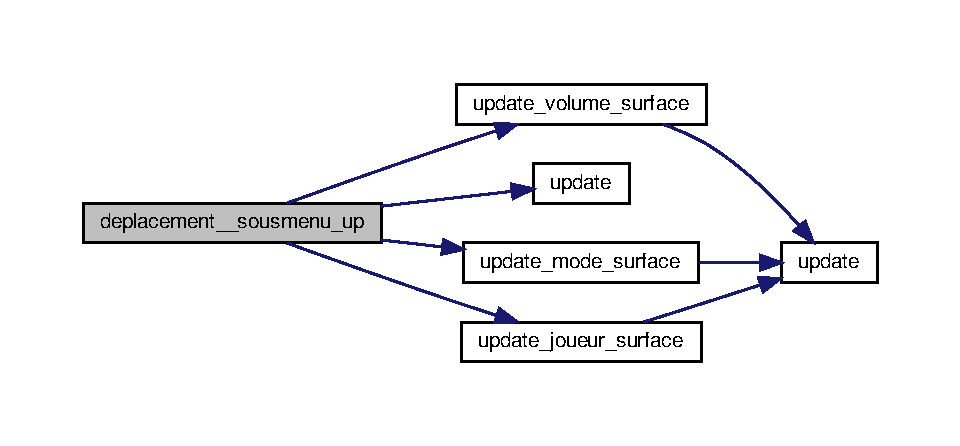
\includegraphics[width=350pt]{menu_8c_a9e2f67419ed3a0025513ff0f1153b4f0_cgraph}
\end{center}
\end{figure}
Here is the caller graph for this function\+:
\nopagebreak
\begin{figure}[H]
\begin{center}
\leavevmode
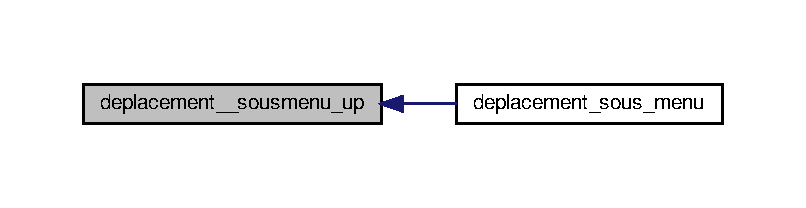
\includegraphics[width=350pt]{menu_8c_a9e2f67419ed3a0025513ff0f1153b4f0_icgraph}
\end{center}
\end{figure}
\mbox{\Hypertarget{menu_8c_ae9a873bbee32be2ae1f56d823111705c}\label{menu_8c_ae9a873bbee32be2ae1f56d823111705c}} 
\index{menu.\+c@{menu.\+c}!deplacement\+\_\+droit\+\_\+gauche\+\_\+joueur@{deplacement\+\_\+droit\+\_\+gauche\+\_\+joueur}}
\index{deplacement\+\_\+droit\+\_\+gauche\+\_\+joueur@{deplacement\+\_\+droit\+\_\+gauche\+\_\+joueur}!menu.\+c@{menu.\+c}}
\subsubsection{\texorpdfstring{deplacement\+\_\+droit\+\_\+gauche\+\_\+joueur()}{deplacement\_droit\_gauche\_joueur()}}
{\footnotesize\ttfamily void deplacement\+\_\+droit\+\_\+gauche\+\_\+joueur (\begin{DoxyParamCaption}\item[{S\+D\+L\+\_\+\+Surface $\ast$}]{screen,  }\item[{Mix\+\_\+\+Chunk $\ast$}]{effect,  }\item[{\hyperlink{structObjet}{Objet}}]{joueur,  }\item[{\hyperlink{structObjet}{Objet}}]{j1,  }\item[{\hyperlink{structObjet}{Objet}}]{j2,  }\item[{int $\ast$}]{position\+\_\+j }\end{DoxyParamCaption})}

Here is the call graph for this function\+:
\nopagebreak
\begin{figure}[H]
\begin{center}
\leavevmode
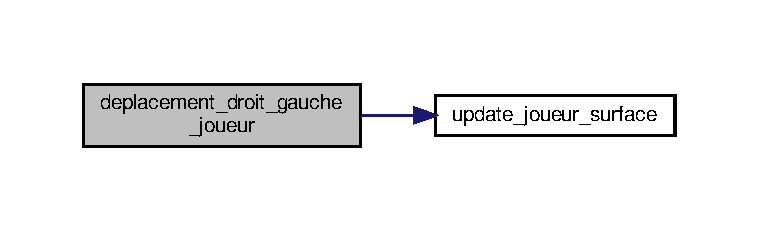
\includegraphics[width=350pt]{menu_8c_ae9a873bbee32be2ae1f56d823111705c_cgraph}
\end{center}
\end{figure}
Here is the caller graph for this function\+:
\nopagebreak
\begin{figure}[H]
\begin{center}
\leavevmode
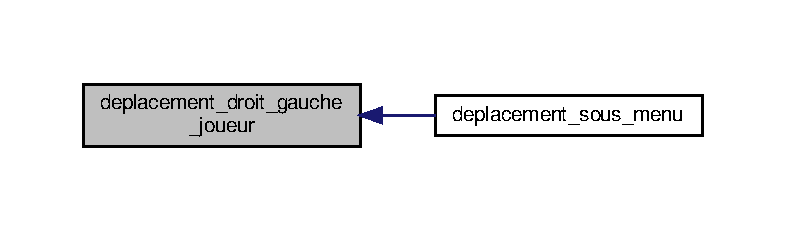
\includegraphics[width=350pt]{menu_8c_ae9a873bbee32be2ae1f56d823111705c_icgraph}
\end{center}
\end{figure}
\mbox{\Hypertarget{menu_8c_ad913190cb846bda4a0ce88df8871f28b}\label{menu_8c_ad913190cb846bda4a0ce88df8871f28b}} 
\index{menu.\+c@{menu.\+c}!deplacement\+\_\+droit\+\_\+gauche\+\_\+mode@{deplacement\+\_\+droit\+\_\+gauche\+\_\+mode}}
\index{deplacement\+\_\+droit\+\_\+gauche\+\_\+mode@{deplacement\+\_\+droit\+\_\+gauche\+\_\+mode}!menu.\+c@{menu.\+c}}
\subsubsection{\texorpdfstring{deplacement\+\_\+droit\+\_\+gauche\+\_\+mode()}{deplacement\_droit\_gauche\_mode()}}
{\footnotesize\ttfamily void deplacement\+\_\+droit\+\_\+gauche\+\_\+mode (\begin{DoxyParamCaption}\item[{S\+D\+L\+\_\+\+Surface $\ast$}]{screen,  }\item[{Mix\+\_\+\+Chunk $\ast$}]{effect,  }\item[{\hyperlink{structObjet}{Objet}}]{mode,  }\item[{\hyperlink{structObjet}{Objet}}]{souris,  }\item[{\hyperlink{structObjet}{Objet}}]{clavier,  }\item[{\hyperlink{structObjet}{Objet}}]{manette,  }\item[{int $\ast$}]{position\+\_\+mode }\end{DoxyParamCaption})}

Here is the call graph for this function\+:
\nopagebreak
\begin{figure}[H]
\begin{center}
\leavevmode
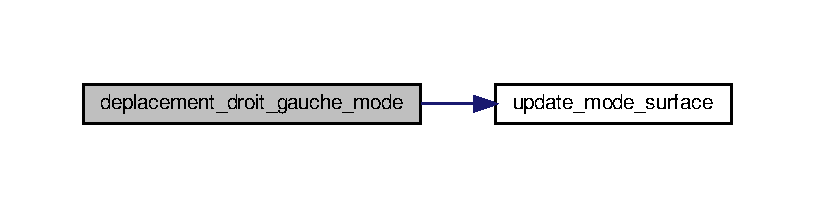
\includegraphics[width=350pt]{menu_8c_ad913190cb846bda4a0ce88df8871f28b_cgraph}
\end{center}
\end{figure}
Here is the caller graph for this function\+:
\nopagebreak
\begin{figure}[H]
\begin{center}
\leavevmode
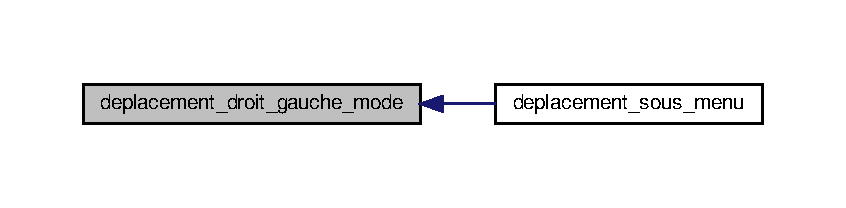
\includegraphics[width=350pt]{menu_8c_ad913190cb846bda4a0ce88df8871f28b_icgraph}
\end{center}
\end{figure}
\mbox{\Hypertarget{menu_8c_a4dda56c63756847abc81ad95418588e9}\label{menu_8c_a4dda56c63756847abc81ad95418588e9}} 
\index{menu.\+c@{menu.\+c}!deplacement\+\_\+droit\+\_\+gauche\+\_\+volume@{deplacement\+\_\+droit\+\_\+gauche\+\_\+volume}}
\index{deplacement\+\_\+droit\+\_\+gauche\+\_\+volume@{deplacement\+\_\+droit\+\_\+gauche\+\_\+volume}!menu.\+c@{menu.\+c}}
\subsubsection{\texorpdfstring{deplacement\+\_\+droit\+\_\+gauche\+\_\+volume()}{deplacement\_droit\_gauche\_volume()}}
{\footnotesize\ttfamily void deplacement\+\_\+droit\+\_\+gauche\+\_\+volume (\begin{DoxyParamCaption}\item[{S\+D\+L\+\_\+\+Surface $\ast$}]{screen,  }\item[{Mix\+\_\+\+Chunk $\ast$}]{effect,  }\item[{\hyperlink{structObjet}{Objet}}]{in\+\_\+sound,  }\item[{\hyperlink{structObjet}{Objet}}]{in\+\_\+sound25,  }\item[{\hyperlink{structObjet}{Objet}}]{in\+\_\+sound50,  }\item[{\hyperlink{structObjet}{Objet}}]{in\+\_\+sound75,  }\item[{\hyperlink{structObjet}{Objet}}]{in\+\_\+sound100,  }\item[{int $\ast$}]{position\+\_\+volume }\end{DoxyParamCaption})}

Here is the call graph for this function\+:
\nopagebreak
\begin{figure}[H]
\begin{center}
\leavevmode
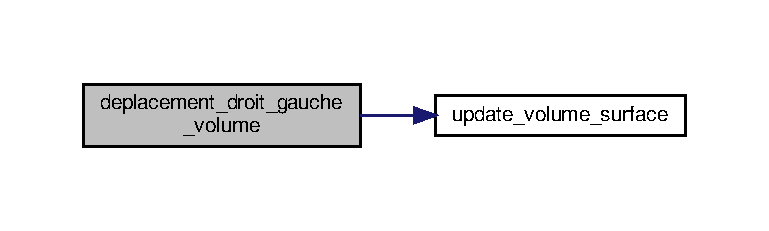
\includegraphics[width=350pt]{menu_8c_a4dda56c63756847abc81ad95418588e9_cgraph}
\end{center}
\end{figure}
Here is the caller graph for this function\+:
\nopagebreak
\begin{figure}[H]
\begin{center}
\leavevmode
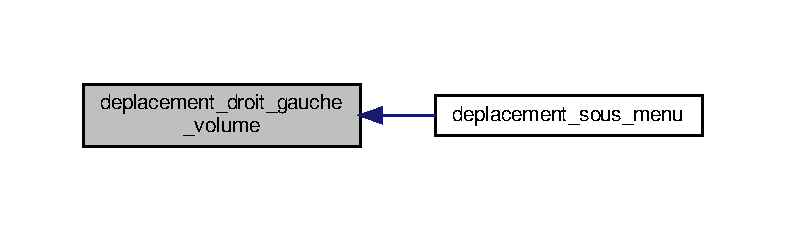
\includegraphics[width=350pt]{menu_8c_a4dda56c63756847abc81ad95418588e9_icgraph}
\end{center}
\end{figure}
\mbox{\Hypertarget{menu_8c_a1bc9078394ad9f78ce5a36a6ffcf2f21}\label{menu_8c_a1bc9078394ad9f78ce5a36a6ffcf2f21}} 
\index{menu.\+c@{menu.\+c}!deplacement\+\_\+sous\+\_\+menu@{deplacement\+\_\+sous\+\_\+menu}}
\index{deplacement\+\_\+sous\+\_\+menu@{deplacement\+\_\+sous\+\_\+menu}!menu.\+c@{menu.\+c}}
\subsubsection{\texorpdfstring{deplacement\+\_\+sous\+\_\+menu()}{deplacement\_sous\_menu()}}
{\footnotesize\ttfamily void deplacement\+\_\+sous\+\_\+menu (\begin{DoxyParamCaption}\item[{S\+D\+L\+\_\+\+Surface $\ast$}]{screen,  }\item[{Mix\+\_\+\+Chunk $\ast$}]{effect,  }\item[{S\+D\+L\+\_\+\+Event}]{event,  }\item[{int $\ast$}]{running2,  }\item[{\hyperlink{structObjet}{Objet}}]{in\+\_\+settings,  }\item[{\hyperlink{structObjet}{Objet}}]{in\+\_\+sound,  }\item[{\hyperlink{structObjet}{Objet}}]{in\+\_\+sound25,  }\item[{\hyperlink{structObjet}{Objet}}]{in\+\_\+sound50,  }\item[{\hyperlink{structObjet}{Objet}}]{in\+\_\+sound75,  }\item[{\hyperlink{structObjet}{Objet}}]{in\+\_\+sound100,  }\item[{int $\ast$}]{position\+\_\+volume,  }\item[{\hyperlink{structObjet}{Objet}}]{credits,  }\item[{\hyperlink{structObjet}{Objet}}]{main\+\_\+menu,  }\item[{\hyperlink{structObjet}{Objet} $\ast$}]{icon,  }\item[{int $\ast$}]{running,  }\item[{int $\ast$}]{curseur,  }\item[{\hyperlink{structObjet}{Objet}}]{game,  }\item[{int $\ast$}]{boolean\+\_\+icon,  }\item[{\hyperlink{structObjet}{Objet}}]{j1,  }\item[{\hyperlink{structObjet}{Objet}}]{j2,  }\item[{\hyperlink{structObjet}{Objet}}]{joueur,  }\item[{\hyperlink{structObjet}{Objet}}]{mode,  }\item[{\hyperlink{structObjet}{Objet}}]{souris,  }\item[{\hyperlink{structObjet}{Objet}}]{clavier,  }\item[{\hyperlink{structObjet}{Objet}}]{manette,  }\item[{int $\ast$}]{position\+\_\+mode,  }\item[{int $\ast$}]{position\+\_\+j }\end{DoxyParamCaption})}

Here is the call graph for this function\+:
\nopagebreak
\begin{figure}[H]
\begin{center}
\leavevmode
\includegraphics[width=350pt]{menu_8c_a1bc9078394ad9f78ce5a36a6ffcf2f21_cgraph}
\end{center}
\end{figure}
\mbox{\Hypertarget{menu_8c_aac902a236492a975286b3efad66b5959}\label{menu_8c_aac902a236492a975286b3efad66b5959}} 
\index{menu.\+c@{menu.\+c}!deplacementmenu\+\_\+down@{deplacementmenu\+\_\+down}}
\index{deplacementmenu\+\_\+down@{deplacementmenu\+\_\+down}!menu.\+c@{menu.\+c}}
\subsubsection{\texorpdfstring{deplacementmenu\+\_\+down()}{deplacementmenu\_down()}}
{\footnotesize\ttfamily void deplacementmenu\+\_\+down (\begin{DoxyParamCaption}\item[{S\+D\+L\+\_\+\+Surface $\ast$}]{screen,  }\item[{Mix\+\_\+\+Chunk $\ast$}]{effect,  }\item[{int $\ast$}]{curseur,  }\item[{\hyperlink{structObjet}{Objet}}]{newgame,  }\item[{\hyperlink{structObjet}{Objet}}]{icon,  }\item[{\hyperlink{structObjet}{Objet}}]{loadgame,  }\item[{\hyperlink{structObjet}{Objet}}]{settings,  }\item[{\hyperlink{structObjet}{Objet}}]{quitter,  }\item[{int $\ast$}]{quitt }\end{DoxyParamCaption})}

Here is the call graph for this function\+:
\nopagebreak
\begin{figure}[H]
\begin{center}
\leavevmode
\includegraphics[width=287pt]{menu_8c_aac902a236492a975286b3efad66b5959_cgraph}
\end{center}
\end{figure}
Here is the caller graph for this function\+:
\nopagebreak
\begin{figure}[H]
\begin{center}
\leavevmode
\includegraphics[width=350pt]{menu_8c_aac902a236492a975286b3efad66b5959_icgraph}
\end{center}
\end{figure}
\mbox{\Hypertarget{menu_8c_aa22c513c93d701f2e2f849693357333e}\label{menu_8c_aa22c513c93d701f2e2f849693357333e}} 
\index{menu.\+c@{menu.\+c}!deplacementmenu\+\_\+up@{deplacementmenu\+\_\+up}}
\index{deplacementmenu\+\_\+up@{deplacementmenu\+\_\+up}!menu.\+c@{menu.\+c}}
\subsubsection{\texorpdfstring{deplacementmenu\+\_\+up()}{deplacementmenu\_up()}}
{\footnotesize\ttfamily void deplacementmenu\+\_\+up (\begin{DoxyParamCaption}\item[{S\+D\+L\+\_\+\+Surface $\ast$}]{screen,  }\item[{Mix\+\_\+\+Chunk $\ast$}]{effect,  }\item[{int $\ast$}]{curseur,  }\item[{\hyperlink{structObjet}{Objet}}]{newgame,  }\item[{\hyperlink{structObjet}{Objet}}]{icon,  }\item[{\hyperlink{structObjet}{Objet}}]{loadgame,  }\item[{\hyperlink{structObjet}{Objet}}]{settings,  }\item[{\hyperlink{structObjet}{Objet}}]{quitter,  }\item[{int $\ast$}]{quitt }\end{DoxyParamCaption})}

Here is the call graph for this function\+:
\nopagebreak
\begin{figure}[H]
\begin{center}
\leavevmode
\includegraphics[width=274pt]{menu_8c_aa22c513c93d701f2e2f849693357333e_cgraph}
\end{center}
\end{figure}
Here is the caller graph for this function\+:
\nopagebreak
\begin{figure}[H]
\begin{center}
\leavevmode
\includegraphics[width=350pt]{menu_8c_aa22c513c93d701f2e2f849693357333e_icgraph}
\end{center}
\end{figure}
\mbox{\Hypertarget{menu_8c_a2268ff186e35842b248248c0c4e8354c}\label{menu_8c_a2268ff186e35842b248248c0c4e8354c}} 
\index{menu.\+c@{menu.\+c}!deplacementmenu\+\_\+up\+\_\+down@{deplacementmenu\+\_\+up\+\_\+down}}
\index{deplacementmenu\+\_\+up\+\_\+down@{deplacementmenu\+\_\+up\+\_\+down}!menu.\+c@{menu.\+c}}
\subsubsection{\texorpdfstring{deplacementmenu\+\_\+up\+\_\+down()}{deplacementmenu\_up\_down()}}
{\footnotesize\ttfamily int deplacementmenu\+\_\+up\+\_\+down (\begin{DoxyParamCaption}\item[{S\+D\+L\+\_\+\+Surface $\ast$}]{screen,  }\item[{S\+D\+L\+\_\+\+Event}]{event,  }\item[{int $\ast$}]{curseur,  }\item[{int $\ast$}]{running,  }\item[{\hyperlink{structObjet}{Objet}}]{newgame,  }\item[{\hyperlink{structObjet}{Objet}}]{loadgame,  }\item[{\hyperlink{structObjet}{Objet}}]{settings,  }\item[{\hyperlink{structObjet}{Objet}}]{quitter,  }\item[{\hyperlink{structObjet}{Objet} $\ast$}]{icon,  }\item[{\hyperlink{structObjet}{Objet}}]{in\+\_\+settings,  }\item[{Mix\+\_\+\+Chunk $\ast$}]{effect,  }\item[{int $\ast$}]{boolean\+\_\+icon,  }\item[{int $\ast$}]{quitt,  }\item[{\hyperlink{structObjet}{Objet}}]{exxit }\end{DoxyParamCaption})}

Here is the call graph for this function\+:
\nopagebreak
\begin{figure}[H]
\begin{center}
\leavevmode
\includegraphics[width=350pt]{menu_8c_a2268ff186e35842b248248c0c4e8354c_cgraph}
\end{center}
\end{figure}
\mbox{\Hypertarget{menu_8c_a6ed81a9b60090a7e012e1c6a57bbbe57}\label{menu_8c_a6ed81a9b60090a7e012e1c6a57bbbe57}} 
\index{menu.\+c@{menu.\+c}!initialiser@{initialiser}}
\index{initialiser@{initialiser}!menu.\+c@{menu.\+c}}
\subsubsection{\texorpdfstring{initialiser()}{initialiser()}}
{\footnotesize\ttfamily void initialiser (\begin{DoxyParamCaption}\item[{\hyperlink{structObjet}{Objet} $\ast$}]{newgame,  }\item[{\hyperlink{structObjet}{Objet} $\ast$}]{loadgame,  }\item[{\hyperlink{structObjet}{Objet} $\ast$}]{settings,  }\item[{\hyperlink{structObjet}{Objet} $\ast$}]{icon,  }\item[{\hyperlink{structObjet}{Objet} $\ast$}]{in\+\_\+sound,  }\item[{\hyperlink{structObjet}{Objet} $\ast$}]{in\+\_\+sound25,  }\item[{\hyperlink{structObjet}{Objet} $\ast$}]{in\+\_\+sound50,  }\item[{\hyperlink{structObjet}{Objet} $\ast$}]{in\+\_\+sound75,  }\item[{\hyperlink{structObjet}{Objet} $\ast$}]{in\+\_\+sound100,  }\item[{\hyperlink{structObjet}{Objet} $\ast$}]{in\+\_\+settings,  }\item[{\hyperlink{structObjet}{Objet} $\ast$}]{credits,  }\item[{\hyperlink{structObjet}{Objet} $\ast$}]{main\+\_\+menu,  }\item[{\hyperlink{structObjet}{Objet} $\ast$}]{quitter,  }\item[{\hyperlink{structObjet}{Objet} $\ast$}]{wexit,  }\item[{\hyperlink{structObjet}{Objet} $\ast$}]{nwexit,  }\item[{\hyperlink{structObjet}{Objet} $\ast$}]{exxit,  }\item[{\hyperlink{structObjet}{Objet} $\ast$}]{game,  }\item[{\hyperlink{structObjet}{Objet} $\ast$}]{j1,  }\item[{\hyperlink{structObjet}{Objet} $\ast$}]{j2,  }\item[{\hyperlink{structObjet}{Objet} $\ast$}]{joueur,  }\item[{\hyperlink{structObjet}{Objet} $\ast$}]{mode,  }\item[{\hyperlink{structObjet}{Objet} $\ast$}]{souris,  }\item[{\hyperlink{structObjet}{Objet} $\ast$}]{clavier,  }\item[{\hyperlink{structObjet}{Objet} $\ast$}]{manette }\end{DoxyParamCaption})}

\mbox{\Hypertarget{menu_8c_aee999999e7b274237009a249b0227564}\label{menu_8c_aee999999e7b274237009a249b0227564}} 
\index{menu.\+c@{menu.\+c}!liberate@{liberate}}
\index{liberate@{liberate}!menu.\+c@{menu.\+c}}
\subsubsection{\texorpdfstring{liberate()}{liberate()}}
{\footnotesize\ttfamily void liberate (\begin{DoxyParamCaption}\item[{\hyperlink{structObjet}{Objet} $\ast$}]{newgame,  }\item[{\hyperlink{structObjet}{Objet} $\ast$}]{loadgame,  }\item[{\hyperlink{structObjet}{Objet} $\ast$}]{settings,  }\item[{\hyperlink{structObjet}{Objet} $\ast$}]{icon,  }\item[{\hyperlink{structObjet}{Objet} $\ast$}]{in\+\_\+sound,  }\item[{\hyperlink{structObjet}{Objet} $\ast$}]{in\+\_\+sound25,  }\item[{\hyperlink{structObjet}{Objet} $\ast$}]{in\+\_\+sound50,  }\item[{\hyperlink{structObjet}{Objet} $\ast$}]{in\+\_\+sound75,  }\item[{\hyperlink{structObjet}{Objet} $\ast$}]{in\+\_\+sound100,  }\item[{\hyperlink{structObjet}{Objet} $\ast$}]{in\+\_\+settings,  }\item[{\hyperlink{structObjet}{Objet} $\ast$}]{credits,  }\item[{\hyperlink{structObjet}{Objet} $\ast$}]{main\+\_\+menu,  }\item[{\hyperlink{structObjet}{Objet} $\ast$}]{quitter,  }\item[{\hyperlink{structObjet}{Objet} $\ast$}]{wexit,  }\item[{\hyperlink{structObjet}{Objet} $\ast$}]{nwexit,  }\item[{\hyperlink{structObjet}{Objet} $\ast$}]{exxit,  }\item[{\hyperlink{structObjet}{Objet} $\ast$}]{game,  }\item[{\hyperlink{structObjet}{Objet} $\ast$}]{j1,  }\item[{\hyperlink{structObjet}{Objet} $\ast$}]{j2,  }\item[{\hyperlink{structObjet}{Objet} $\ast$}]{joueur,  }\item[{\hyperlink{structObjet}{Objet} $\ast$}]{mode,  }\item[{\hyperlink{structObjet}{Objet} $\ast$}]{souris,  }\item[{\hyperlink{structObjet}{Objet} $\ast$}]{clavier,  }\item[{\hyperlink{structObjet}{Objet} $\ast$}]{manette }\end{DoxyParamCaption})}

\mbox{\Hypertarget{menu_8c_a0ab41f2cf0da8abca3dafab82382517f}\label{menu_8c_a0ab41f2cf0da8abca3dafab82382517f}} 
\index{menu.\+c@{menu.\+c}!motion\+\_\+souris\+\_\+sousmenu@{motion\+\_\+souris\+\_\+sousmenu}}
\index{motion\+\_\+souris\+\_\+sousmenu@{motion\+\_\+souris\+\_\+sousmenu}!menu.\+c@{menu.\+c}}
\subsubsection{\texorpdfstring{motion\+\_\+souris\+\_\+sousmenu()}{motion\_souris\_sousmenu()}}
{\footnotesize\ttfamily void motion\+\_\+souris\+\_\+sousmenu (\begin{DoxyParamCaption}\item[{S\+D\+L\+\_\+\+Surface $\ast$}]{screen,  }\item[{S\+D\+L\+\_\+\+Event}]{event,  }\item[{Mix\+\_\+\+Chunk $\ast$}]{effect,  }\item[{int $\ast$}]{curseur,  }\item[{\hyperlink{structObjet}{Objet}}]{in\+\_\+sound,  }\item[{\hyperlink{structObjet}{Objet}}]{in\+\_\+sound25,  }\item[{\hyperlink{structObjet}{Objet}}]{in\+\_\+sound50,  }\item[{\hyperlink{structObjet}{Objet}}]{in\+\_\+sound75,  }\item[{\hyperlink{structObjet}{Objet}}]{in\+\_\+sound100,  }\item[{int}]{position\+\_\+volume,  }\item[{\hyperlink{structObjet}{Objet}}]{icon,  }\item[{\hyperlink{structObjet}{Objet}}]{credits,  }\item[{\hyperlink{structObjet}{Objet}}]{main\+\_\+menu,  }\item[{\hyperlink{structObjet}{Objet}}]{j1,  }\item[{\hyperlink{structObjet}{Objet}}]{j2,  }\item[{\hyperlink{structObjet}{Objet}}]{joueur,  }\item[{\hyperlink{structObjet}{Objet}}]{mode,  }\item[{\hyperlink{structObjet}{Objet}}]{souris,  }\item[{\hyperlink{structObjet}{Objet}}]{clavier,  }\item[{\hyperlink{structObjet}{Objet}}]{manette,  }\item[{int}]{position\+\_\+mode,  }\item[{int}]{position\+\_\+j }\end{DoxyParamCaption})}

Here is the call graph for this function\+:
\nopagebreak
\begin{figure}[H]
\begin{center}
\leavevmode
\includegraphics[width=350pt]{menu_8c_a0ab41f2cf0da8abca3dafab82382517f_cgraph}
\end{center}
\end{figure}
Here is the caller graph for this function\+:
\nopagebreak
\begin{figure}[H]
\begin{center}
\leavevmode
\includegraphics[width=350pt]{menu_8c_a0ab41f2cf0da8abca3dafab82382517f_icgraph}
\end{center}
\end{figure}
\mbox{\Hypertarget{menu_8c_a01fee34ecc94975dc64a8b97eec33629}\label{menu_8c_a01fee34ecc94975dc64a8b97eec33629}} 
\index{menu.\+c@{menu.\+c}!mouse\+\_\+motion\+\_\+main\+\_\+menu@{mouse\+\_\+motion\+\_\+main\+\_\+menu}}
\index{mouse\+\_\+motion\+\_\+main\+\_\+menu@{mouse\+\_\+motion\+\_\+main\+\_\+menu}!menu.\+c@{menu.\+c}}
\subsubsection{\texorpdfstring{mouse\+\_\+motion\+\_\+main\+\_\+menu()}{mouse\_motion\_main\_menu()}}
{\footnotesize\ttfamily void mouse\+\_\+motion\+\_\+main\+\_\+menu (\begin{DoxyParamCaption}\item[{S\+D\+L\+\_\+\+Surface $\ast$}]{screen,  }\item[{S\+D\+L\+\_\+\+Event}]{event,  }\item[{Mix\+\_\+\+Chunk $\ast$}]{effect,  }\item[{int $\ast$}]{curseur,  }\item[{\hyperlink{structObjet}{Objet}}]{newgame,  }\item[{\hyperlink{structObjet}{Objet}}]{icon,  }\item[{\hyperlink{structObjet}{Objet}}]{loadgame,  }\item[{\hyperlink{structObjet}{Objet}}]{settings,  }\item[{\hyperlink{structObjet}{Objet}}]{quitter,  }\item[{int $\ast$}]{quitt }\end{DoxyParamCaption})}

Here is the call graph for this function\+:
\nopagebreak
\begin{figure}[H]
\begin{center}
\leavevmode
\includegraphics[width=350pt]{menu_8c_a01fee34ecc94975dc64a8b97eec33629_cgraph}
\end{center}
\end{figure}
Here is the caller graph for this function\+:
\nopagebreak
\begin{figure}[H]
\begin{center}
\leavevmode
\includegraphics[width=350pt]{menu_8c_a01fee34ecc94975dc64a8b97eec33629_icgraph}
\end{center}
\end{figure}
\mbox{\Hypertarget{menu_8c_af4b216a06daa438e8c9d0a41df4d1cd9}\label{menu_8c_af4b216a06daa438e8c9d0a41df4d1cd9}} 
\index{menu.\+c@{menu.\+c}!quitter\+\_\+oui\+\_\+non@{quitter\+\_\+oui\+\_\+non}}
\index{quitter\+\_\+oui\+\_\+non@{quitter\+\_\+oui\+\_\+non}!menu.\+c@{menu.\+c}}
\subsubsection{\texorpdfstring{quitter\+\_\+oui\+\_\+non()}{quitter\_oui\_non()}}
{\footnotesize\ttfamily void quitter\+\_\+oui\+\_\+non (\begin{DoxyParamCaption}\item[{S\+D\+L\+\_\+\+Surface $\ast$}]{screen,  }\item[{S\+D\+L\+\_\+\+Event}]{event,  }\item[{int $\ast$}]{running,  }\item[{int $\ast$}]{running2,  }\item[{int $\ast$}]{running3,  }\item[{\hyperlink{structObjet}{Objet}}]{quitter,  }\item[{\hyperlink{structObjet}{Objet}}]{icon,  }\item[{\hyperlink{structObjet}{Objet}}]{wexit,  }\item[{\hyperlink{structObjet}{Objet}}]{nwexit,  }\item[{int $\ast$}]{test,  }\item[{int $\ast$}]{test\+\_\+s }\end{DoxyParamCaption})}

Here is the call graph for this function\+:
\nopagebreak
\begin{figure}[H]
\begin{center}
\leavevmode
\includegraphics[width=306pt]{menu_8c_af4b216a06daa438e8c9d0a41df4d1cd9_cgraph}
\end{center}
\end{figure}
\mbox{\Hypertarget{menu_8c_a74ff2595edb8cb817eeab72f1662171f}\label{menu_8c_a74ff2595edb8cb817eeab72f1662171f}} 
\index{menu.\+c@{menu.\+c}!setup@{setup}}
\index{setup@{setup}!menu.\+c@{menu.\+c}}
\subsubsection{\texorpdfstring{setup()}{setup()}}
{\footnotesize\ttfamily void setup (\begin{DoxyParamCaption}\item[{S\+D\+L\+\_\+\+Surface $\ast$}]{screen,  }\item[{\hyperlink{structObjet}{Objet} $\ast$}]{game,  }\item[{\hyperlink{structObjet}{Objet} $\ast$}]{icon }\end{DoxyParamCaption})}

\mbox{\Hypertarget{menu_8c_a989655a408019727ed1e4f69cc6cb4e7}\label{menu_8c_a989655a408019727ed1e4f69cc6cb4e7}} 
\index{menu.\+c@{menu.\+c}!update@{update}}
\index{update@{update}!menu.\+c@{menu.\+c}}
\subsubsection{\texorpdfstring{update()}{update()}}
{\footnotesize\ttfamily void update (\begin{DoxyParamCaption}\item[{S\+D\+L\+\_\+\+Surface $\ast$}]{screen,  }\item[{\hyperlink{structObjet}{Objet} $\ast$}]{surface1,  }\item[{\hyperlink{structObjet}{Objet} $\ast$}]{surface2 }\end{DoxyParamCaption})}

Here is the caller graph for this function\+:
\nopagebreak
\begin{figure}[H]
\begin{center}
\leavevmode
\includegraphics[width=350pt]{menu_8c_a989655a408019727ed1e4f69cc6cb4e7_icgraph}
\end{center}
\end{figure}
\mbox{\Hypertarget{menu_8c_aacfe086068def17eb2d10ee72c726062}\label{menu_8c_aacfe086068def17eb2d10ee72c726062}} 
\index{menu.\+c@{menu.\+c}!update\+\_\+joueur\+\_\+surface@{update\+\_\+joueur\+\_\+surface}}
\index{update\+\_\+joueur\+\_\+surface@{update\+\_\+joueur\+\_\+surface}!menu.\+c@{menu.\+c}}
\subsubsection{\texorpdfstring{update\+\_\+joueur\+\_\+surface()}{update\_joueur\_surface()}}
{\footnotesize\ttfamily void update\+\_\+joueur\+\_\+surface (\begin{DoxyParamCaption}\item[{S\+D\+L\+\_\+\+Surface $\ast$}]{screen,  }\item[{Mix\+\_\+\+Chunk $\ast$}]{effect,  }\item[{\hyperlink{structObjet}{Objet}}]{joueur,  }\item[{\hyperlink{structObjet}{Objet}}]{j1,  }\item[{\hyperlink{structObjet}{Objet}}]{j2,  }\item[{int}]{position\+\_\+j }\end{DoxyParamCaption})}

Here is the call graph for this function\+:
\nopagebreak
\begin{figure}[H]
\begin{center}
\leavevmode
\includegraphics[width=277pt]{menu_8c_aacfe086068def17eb2d10ee72c726062_cgraph}
\end{center}
\end{figure}
Here is the caller graph for this function\+:
\nopagebreak
\begin{figure}[H]
\begin{center}
\leavevmode
\includegraphics[width=350pt]{menu_8c_aacfe086068def17eb2d10ee72c726062_icgraph}
\end{center}
\end{figure}
\mbox{\Hypertarget{menu_8c_acbff537c998bef21d8aec4663b32500d}\label{menu_8c_acbff537c998bef21d8aec4663b32500d}} 
\index{menu.\+c@{menu.\+c}!update\+\_\+mode\+\_\+surface@{update\+\_\+mode\+\_\+surface}}
\index{update\+\_\+mode\+\_\+surface@{update\+\_\+mode\+\_\+surface}!menu.\+c@{menu.\+c}}
\subsubsection{\texorpdfstring{update\+\_\+mode\+\_\+surface()}{update\_mode\_surface()}}
{\footnotesize\ttfamily void update\+\_\+mode\+\_\+surface (\begin{DoxyParamCaption}\item[{S\+D\+L\+\_\+\+Surface $\ast$}]{screen,  }\item[{Mix\+\_\+\+Chunk $\ast$}]{effect,  }\item[{\hyperlink{structObjet}{Objet}}]{mode,  }\item[{\hyperlink{structObjet}{Objet}}]{souris,  }\item[{\hyperlink{structObjet}{Objet}}]{clavier,  }\item[{\hyperlink{structObjet}{Objet}}]{manette,  }\item[{int}]{position\+\_\+mode }\end{DoxyParamCaption})}

Here is the call graph for this function\+:
\nopagebreak
\begin{figure}[H]
\begin{center}
\leavevmode
\includegraphics[width=275pt]{menu_8c_acbff537c998bef21d8aec4663b32500d_cgraph}
\end{center}
\end{figure}
Here is the caller graph for this function\+:
\nopagebreak
\begin{figure}[H]
\begin{center}
\leavevmode
\includegraphics[width=350pt]{menu_8c_acbff537c998bef21d8aec4663b32500d_icgraph}
\end{center}
\end{figure}
\mbox{\Hypertarget{menu_8c_aafa1723742aaf10400d1226394e81e31}\label{menu_8c_aafa1723742aaf10400d1226394e81e31}} 
\index{menu.\+c@{menu.\+c}!update\+\_\+volume\+\_\+surface@{update\+\_\+volume\+\_\+surface}}
\index{update\+\_\+volume\+\_\+surface@{update\+\_\+volume\+\_\+surface}!menu.\+c@{menu.\+c}}
\subsubsection{\texorpdfstring{update\+\_\+volume\+\_\+surface()}{update\_volume\_surface()}}
{\footnotesize\ttfamily void update\+\_\+volume\+\_\+surface (\begin{DoxyParamCaption}\item[{S\+D\+L\+\_\+\+Surface $\ast$}]{screen,  }\item[{Mix\+\_\+\+Chunk $\ast$}]{effect,  }\item[{\hyperlink{structObjet}{Objet}}]{in\+\_\+sound,  }\item[{\hyperlink{structObjet}{Objet}}]{in\+\_\+sound25,  }\item[{\hyperlink{structObjet}{Objet}}]{in\+\_\+sound50,  }\item[{\hyperlink{structObjet}{Objet}}]{in\+\_\+sound75,  }\item[{\hyperlink{structObjet}{Objet}}]{in\+\_\+sound100,  }\item[{int}]{position\+\_\+volume }\end{DoxyParamCaption})}

Here is the call graph for this function\+:
\nopagebreak
\begin{figure}[H]
\begin{center}
\leavevmode
\includegraphics[width=282pt]{menu_8c_aafa1723742aaf10400d1226394e81e31_cgraph}
\end{center}
\end{figure}
Here is the caller graph for this function\+:
\nopagebreak
\begin{figure}[H]
\begin{center}
\leavevmode
\includegraphics[width=350pt]{menu_8c_aafa1723742aaf10400d1226394e81e31_icgraph}
\end{center}
\end{figure}
\mbox{\Hypertarget{menu_8c_abe842397d22ae8a423936cc41bba4845}\label{menu_8c_abe842397d22ae8a423936cc41bba4845}} 
\index{menu.\+c@{menu.\+c}!verif\+\_\+motion\+\_\+surface@{verif\+\_\+motion\+\_\+surface}}
\index{verif\+\_\+motion\+\_\+surface@{verif\+\_\+motion\+\_\+surface}!menu.\+c@{menu.\+c}}
\subsubsection{\texorpdfstring{verif\+\_\+motion\+\_\+surface()}{verif\_motion\_surface()}}
{\footnotesize\ttfamily int verif\+\_\+motion\+\_\+surface (\begin{DoxyParamCaption}\item[{S\+D\+L\+\_\+\+Event}]{event,  }\item[{\hyperlink{structObjet}{Objet}}]{surface }\end{DoxyParamCaption})}

Here is the caller graph for this function\+:
\nopagebreak
\begin{figure}[H]
\begin{center}
\leavevmode
\includegraphics[width=350pt]{menu_8c_abe842397d22ae8a423936cc41bba4845_icgraph}
\end{center}
\end{figure}

\hypertarget{menu_8h}{}\section{menu.\+h File Reference}
\label{menu_8h}\index{menu.\+h@{menu.\+h}}
{\ttfamily \#include $<$S\+D\+L/\+S\+D\+L.\+h$>$}\newline
{\ttfamily \#include $<$S\+D\+L/\+S\+D\+L\+\_\+image.\+h$>$}\newline
{\ttfamily \#include $<$S\+D\+L/\+S\+D\+L\+\_\+ttf.\+h$>$}\newline
{\ttfamily \#include \char`\"{}S\+D\+L/\+S\+D\+L\+\_\+mixer.\+h\char`\"{}}\newline
Include dependency graph for menu.\+h\+:
\nopagebreak
\begin{figure}[H]
\begin{center}
\leavevmode
\includegraphics[width=350pt]{menu_8h__incl}
\end{center}
\end{figure}
This graph shows which files directly or indirectly include this file\+:
\nopagebreak
\begin{figure}[H]
\begin{center}
\leavevmode
\includegraphics[width=293pt]{menu_8h__dep__incl}
\end{center}
\end{figure}
\subsection*{Classes}
\begin{DoxyCompactItemize}
\item 
struct \hyperlink{structObjet}{Objet}
\end{DoxyCompactItemize}
\subsection*{Macros}
\begin{DoxyCompactItemize}
\item 
\#define \hyperlink{menu_8h_a667b04d7fb6ef46db4da4af554c5b6f7}{width}~1213
\item 
\#define \hyperlink{menu_8h_a64f9f90ece96c7bab4aee3deacf170e0}{height}~760
\item 
\#define \hyperlink{menu_8h_a214880d0db4c911c3789f7f0441ace2e}{n\+\_\+w}~341
\item 
\#define \hyperlink{menu_8h_af98ecf802ce354c9abc68c596e99d71c}{n\+\_\+h}~174
\item 
\#define \hyperlink{menu_8h_a5a608eae929eed67ad951a0aa83c3623}{s\+\_\+w}~341
\item 
\#define \hyperlink{menu_8h_a0d88a0c19bc91060259b1e2e4b0743f8}{s\+\_\+h}~126
\item 
\#define \hyperlink{menu_8h_a8b14141a2dd5dc1395d09736db79e47b}{e\+\_\+w}~341
\item 
\#define \hyperlink{menu_8h_a20c906935baccc6a4ba20eb3b99533cc}{e\+\_\+h}~116
\item 
\#define \hyperlink{menu_8h_a0a094da52c7b7237984b3c64d3b958fb}{sound\+\_\+w}~55
\item 
\#define \hyperlink{menu_8h_a2beaea74698a9cff855848c6423e75d6}{sound\+\_\+h}~55
\item 
\#define \hyperlink{menu_8h_a3055bb315de980581f52c897633690cb}{i\+\_\+s\+\_\+w}~220
\item 
\#define \hyperlink{menu_8h_a78b6a892aff15d70fa393af14f34b02f}{i\+\_\+s\+\_\+h}~24
\item 
\#define \hyperlink{menu_8h_a0c0182773ab945d860363c19ce5e6b16}{yn\+\_\+w}~384
\item 
\#define \hyperlink{menu_8h_a86eaae2f6756a4156d3b6689435920e7}{yn\+\_\+h}~151
\item 
\#define \hyperlink{menu_8h_a5c3da54e74936e63c5211b3daa26aea4}{mp\+\_\+w}~40
\item 
\#define \hyperlink{menu_8h_a5a07612d67d9d3789e8c029ee72dc528}{mp\+\_\+h}~40
\item 
\#define \hyperlink{menu_8h_ae4203e18a1f2645319ac33bbd67effd8}{b\+\_\+w}~194
\item 
\#define \hyperlink{menu_8h_adc071059a567c7c6e9266ed452a0a160}{b\+\_\+h}~72
\item 
\#define \hyperlink{menu_8h_ab1d14c6bf3badfd34103cb87583a9aaf}{y\+\_\+w}~211
\item 
\#define \hyperlink{menu_8h_a35aaeddde27b13eac32da3a682e9fd1a}{y\+\_\+h}~72
\item 
\#define \hyperlink{menu_8h_af5429d5c2b325d09703cadf7976553c3}{j\+\_\+w}~148
\item 
\#define \hyperlink{menu_8h_adcc0fa4a76eb752eb72ce8d334a712e2}{j\+\_\+h}~40
\item 
\#define \hyperlink{menu_8h_a2e3a3f4b838d176642e1426f0b5df46d}{m\+\_\+w}~236
\item 
\#define \hyperlink{menu_8h_aa89d69a980b91323841a3d9bca032693}{m\+\_\+h}~60
\item 
\#define \hyperlink{menu_8h_a50d81837cd29022744d2b32f1f06b60d}{so\+\_\+w}~276
\item 
\#define \hyperlink{menu_8h_a049bbfe5380e12ef05213113498d366a}{so\+\_\+h}~30
\item 
\#define \hyperlink{menu_8h_ad5f4dee4d5a4a2eca68424c15e2f09f2}{c\+\_\+w}~273
\item 
\#define \hyperlink{menu_8h_a5959229f5bef071913c5008f661cef03}{c\+\_\+h}~122
\item 
\#define \hyperlink{menu_8h_a27f08c1666d07b35cb26bca79da1aecd}{ma\+\_\+w}~272
\item 
\#define \hyperlink{menu_8h_a1be0e8e05fc48a98c9da1e7b27ce3fca}{ma\+\_\+h}~122
\end{DoxyCompactItemize}
\subsection*{Functions}
\begin{DoxyCompactItemize}
\item 
void \hyperlink{menu_8h_a6ed81a9b60090a7e012e1c6a57bbbe57}{initialiser} (\hyperlink{structObjet}{Objet} $\ast$newgame, \hyperlink{structObjet}{Objet} $\ast$loadgame, \hyperlink{structObjet}{Objet} $\ast$settings, \hyperlink{structObjet}{Objet} $\ast$icon, \hyperlink{structObjet}{Objet} $\ast$in\+\_\+sound, \hyperlink{structObjet}{Objet} $\ast$in\+\_\+sound25, \hyperlink{structObjet}{Objet} $\ast$in\+\_\+sound50, \hyperlink{structObjet}{Objet} $\ast$in\+\_\+sound75, \hyperlink{structObjet}{Objet} $\ast$in\+\_\+sound100, \hyperlink{structObjet}{Objet} $\ast$in\+\_\+settings, \hyperlink{structObjet}{Objet} $\ast$credits, \hyperlink{structObjet}{Objet} $\ast$main\+\_\+menu, \hyperlink{structObjet}{Objet} $\ast$quitter, \hyperlink{structObjet}{Objet} $\ast$wexit, \hyperlink{structObjet}{Objet} $\ast$nwexit, \hyperlink{structObjet}{Objet} $\ast$exxit, \hyperlink{structObjet}{Objet} $\ast$game, \hyperlink{structObjet}{Objet} $\ast$j1, \hyperlink{structObjet}{Objet} $\ast$j2, \hyperlink{structObjet}{Objet} $\ast$joueur, \hyperlink{structObjet}{Objet} $\ast$mode, \hyperlink{structObjet}{Objet} $\ast$souris, \hyperlink{structObjet}{Objet} $\ast$clavier, \hyperlink{structObjet}{Objet} $\ast$manette)
\item 
void \hyperlink{menu_8h_a3dbb891384f41b43e738a7aacdf9c39b}{setup} (S\+D\+L\+\_\+\+Surface $\ast$screen, \hyperlink{structObjet}{Objet} $\ast$game, \hyperlink{structObjet}{Objet} $\ast$y\+\_\+icon)
\item 
int \hyperlink{menu_8h_abe842397d22ae8a423936cc41bba4845}{verif\+\_\+motion\+\_\+surface} (S\+D\+L\+\_\+\+Event event, \hyperlink{structObjet}{Objet} surface)
\item 
void \hyperlink{menu_8h_a989655a408019727ed1e4f69cc6cb4e7}{update} (S\+D\+L\+\_\+\+Surface $\ast$screen, \hyperlink{structObjet}{Objet} $\ast$surface1, \hyperlink{structObjet}{Objet} $\ast$surface2)
\item 
void \hyperlink{menu_8h_a3e090d5d0aab33682e1a4eb763c150fd}{liberate} (\hyperlink{structObjet}{Objet} $\ast$newgame, \hyperlink{structObjet}{Objet} $\ast$loadgame, \hyperlink{structObjet}{Objet} $\ast$settings, \hyperlink{structObjet}{Objet} $\ast$y\+\_\+icon, \hyperlink{structObjet}{Objet} $\ast$in\+\_\+sound, \hyperlink{structObjet}{Objet} $\ast$in\+\_\+sound25, \hyperlink{structObjet}{Objet} $\ast$in\+\_\+sound50, \hyperlink{structObjet}{Objet} $\ast$in\+\_\+sound75, \hyperlink{structObjet}{Objet} $\ast$in\+\_\+sound100, \hyperlink{structObjet}{Objet} $\ast$in\+\_\+settings, \hyperlink{structObjet}{Objet} $\ast$credits, \hyperlink{structObjet}{Objet} $\ast$main\+\_\+menu, \hyperlink{structObjet}{Objet} $\ast$quitter, \hyperlink{structObjet}{Objet} $\ast$wexit, \hyperlink{structObjet}{Objet} $\ast$nwexit, \hyperlink{structObjet}{Objet} $\ast$exxit, \hyperlink{structObjet}{Objet} $\ast$game, \hyperlink{structObjet}{Objet} $\ast$j1, \hyperlink{structObjet}{Objet} $\ast$j2, \hyperlink{structObjet}{Objet} $\ast$joueur, \hyperlink{structObjet}{Objet} $\ast$mode, \hyperlink{structObjet}{Objet} $\ast$souris, \hyperlink{structObjet}{Objet} $\ast$clavier, \hyperlink{structObjet}{Objet} $\ast$manette)
\item 
void \hyperlink{menu_8h_aa78a832057159b053dc97bc50aaa2f6f}{clic\+\_\+souris\+\_\+menu\+\_\+principale} (S\+D\+L\+\_\+\+Surface $\ast$screen, S\+D\+L\+\_\+\+Event event, int curseur, \hyperlink{structObjet}{Objet} newgame, \hyperlink{structObjet}{Objet} loadgame, \hyperlink{structObjet}{Objet} settings, \hyperlink{structObjet}{Objet} in\+\_\+settings, \hyperlink{structObjet}{Objet} $\ast$icon, \hyperlink{structObjet}{Objet} quitter, int $\ast$in, int $\ast$running, int $\ast$boolean\+\_\+icon, int $\ast$quitt, \hyperlink{structObjet}{Objet} exxit)
\item 
void \hyperlink{menu_8h_a5237d05ef4f188f61d5150e4f9ae5114}{clic\+\_\+entrer\+\_\+menu\+\_\+principale} (S\+D\+L\+\_\+\+Surface $\ast$screen, \hyperlink{structObjet}{Objet} in\+\_\+settings, \hyperlink{structObjet}{Objet} icon, Mix\+\_\+\+Chunk $\ast$effect, int curseur, int $\ast$in, int $\ast$running, int $\ast$quitt, \hyperlink{structObjet}{Objet} exxit)
\item 
void \hyperlink{menu_8h_a01fee34ecc94975dc64a8b97eec33629}{mouse\+\_\+motion\+\_\+main\+\_\+menu} (S\+D\+L\+\_\+\+Surface $\ast$screen, S\+D\+L\+\_\+\+Event event, Mix\+\_\+\+Chunk $\ast$effect, int $\ast$curseur, \hyperlink{structObjet}{Objet} newgame, \hyperlink{structObjet}{Objet} icon, \hyperlink{structObjet}{Objet} loadgame, \hyperlink{structObjet}{Objet} settings, \hyperlink{structObjet}{Objet} quitter, int $\ast$quitt)
\item 
void \hyperlink{menu_8h_aac902a236492a975286b3efad66b5959}{deplacementmenu\+\_\+down} (S\+D\+L\+\_\+\+Surface $\ast$screen, Mix\+\_\+\+Chunk $\ast$effect, int $\ast$curseur, \hyperlink{structObjet}{Objet} newgame, \hyperlink{structObjet}{Objet} icon, \hyperlink{structObjet}{Objet} loadgame, \hyperlink{structObjet}{Objet} settings, \hyperlink{structObjet}{Objet} quitter, int $\ast$quitt)
\item 
void \hyperlink{menu_8h_aa22c513c93d701f2e2f849693357333e}{deplacementmenu\+\_\+up} (S\+D\+L\+\_\+\+Surface $\ast$screen, Mix\+\_\+\+Chunk $\ast$effect, int $\ast$curseur, \hyperlink{structObjet}{Objet} newgame, \hyperlink{structObjet}{Objet} icon, \hyperlink{structObjet}{Objet} loadgame, \hyperlink{structObjet}{Objet} settings, \hyperlink{structObjet}{Objet} quitter, int $\ast$quitt)
\item 
int \hyperlink{menu_8h_a26c3bc20b4d8698bc446325652be4fd1}{deplacementmenu\+\_\+up\+\_\+down} (S\+D\+L\+\_\+\+Surface $\ast$screen, S\+D\+L\+\_\+\+Event event, int $\ast$curseur, int $\ast$running, \hyperlink{structObjet}{Objet} newgame, \hyperlink{structObjet}{Objet} loadgame, \hyperlink{structObjet}{Objet} settings, \hyperlink{structObjet}{Objet} quitter, \hyperlink{structObjet}{Objet} $\ast$icon, \hyperlink{structObjet}{Objet} game, Mix\+\_\+\+Chunk $\ast$effect, int $\ast$boolean\+\_\+icon, int $\ast$quitt, \hyperlink{structObjet}{Objet} exxit)
\item 
void \hyperlink{menu_8h_a84db6326acd1f67541347734b3a42729}{deplacement\+\_\+\+\_\+sousmenu\+\_\+down} (S\+D\+L\+\_\+\+Surface $\ast$screen, Mix\+\_\+\+Chunk $\ast$effect, int $\ast$curseur, \hyperlink{structObjet}{Objet} in\+\_\+sound, \hyperlink{structObjet}{Objet} in\+\_\+sound25, \hyperlink{structObjet}{Objet} in\+\_\+sound50, \hyperlink{structObjet}{Objet} in\+\_\+sound75, \hyperlink{structObjet}{Objet} in\+\_\+sound100, int position\+\_\+volume, \hyperlink{structObjet}{Objet} icon, \hyperlink{structObjet}{Objet} credits, \hyperlink{structObjet}{Objet} main\+\_\+menu, \hyperlink{structObjet}{Objet} j1, \hyperlink{structObjet}{Objet} j2, \hyperlink{structObjet}{Objet} joueur, \hyperlink{structObjet}{Objet} mode, \hyperlink{structObjet}{Objet} souris, \hyperlink{structObjet}{Objet} clavier, \hyperlink{structObjet}{Objet} manette, int position\+\_\+mode, int position\+\_\+j)
\item 
void \hyperlink{menu_8h_a9e2f67419ed3a0025513ff0f1153b4f0}{deplacement\+\_\+\+\_\+sousmenu\+\_\+up} (S\+D\+L\+\_\+\+Surface $\ast$screen, Mix\+\_\+\+Chunk $\ast$effect, int $\ast$curseur, \hyperlink{structObjet}{Objet} in\+\_\+sound, \hyperlink{structObjet}{Objet} in\+\_\+sound25, \hyperlink{structObjet}{Objet} in\+\_\+sound50, \hyperlink{structObjet}{Objet} in\+\_\+sound75, \hyperlink{structObjet}{Objet} in\+\_\+sound100, int position\+\_\+volume, \hyperlink{structObjet}{Objet} icon, \hyperlink{structObjet}{Objet} credits, \hyperlink{structObjet}{Objet} main\+\_\+menu, \hyperlink{structObjet}{Objet} j1, \hyperlink{structObjet}{Objet} j2, \hyperlink{structObjet}{Objet} joueur, \hyperlink{structObjet}{Objet} mode, \hyperlink{structObjet}{Objet} souris, \hyperlink{structObjet}{Objet} clavier, \hyperlink{structObjet}{Objet} manette, int position\+\_\+mode, int position\+\_\+j)
\item 
void \hyperlink{menu_8h_aafa1723742aaf10400d1226394e81e31}{update\+\_\+volume\+\_\+surface} (S\+D\+L\+\_\+\+Surface $\ast$screen, Mix\+\_\+\+Chunk $\ast$effect, \hyperlink{structObjet}{Objet} in\+\_\+sound, \hyperlink{structObjet}{Objet} in\+\_\+sound25, \hyperlink{structObjet}{Objet} in\+\_\+sound50, \hyperlink{structObjet}{Objet} in\+\_\+sound75, \hyperlink{structObjet}{Objet} in\+\_\+sound100, int position\+\_\+volume)
\item 
void \hyperlink{menu_8h_a0ab41f2cf0da8abca3dafab82382517f}{motion\+\_\+souris\+\_\+sousmenu} (S\+D\+L\+\_\+\+Surface $\ast$screen, S\+D\+L\+\_\+\+Event event, Mix\+\_\+\+Chunk $\ast$effect, int $\ast$curseur, \hyperlink{structObjet}{Objet} in\+\_\+sound, \hyperlink{structObjet}{Objet} in\+\_\+sound25, \hyperlink{structObjet}{Objet} in\+\_\+sound50, \hyperlink{structObjet}{Objet} in\+\_\+sound75, \hyperlink{structObjet}{Objet} in\+\_\+sound100, int position\+\_\+volume, \hyperlink{structObjet}{Objet} icon, \hyperlink{structObjet}{Objet} credits, \hyperlink{structObjet}{Objet} main\+\_\+menu, \hyperlink{structObjet}{Objet} j1, \hyperlink{structObjet}{Objet} j2, \hyperlink{structObjet}{Objet} joueur, \hyperlink{structObjet}{Objet} mode, \hyperlink{structObjet}{Objet} souris, \hyperlink{structObjet}{Objet} clavier, \hyperlink{structObjet}{Objet} manette, int position\+\_\+mode, int position\+\_\+j)
\item 
void \hyperlink{menu_8h_a7c3b364505423b6ced8dd8ffdb434c13}{clic\+\_\+souris\+\_\+sousmenu} (S\+D\+L\+\_\+\+Surface $\ast$screen, \hyperlink{structObjet}{Objet} $\ast$icon, S\+D\+L\+\_\+\+Event event, int curseur, \hyperlink{structObjet}{Objet} in\+\_\+sound, \hyperlink{structObjet}{Objet} credits, \hyperlink{structObjet}{Objet} main\+\_\+menu, int $\ast$running2, \hyperlink{structObjet}{Objet} game, int $\ast$boolean\+\_\+icon, \hyperlink{structObjet}{Objet} j1, \hyperlink{structObjet}{Objet} j2, \hyperlink{structObjet}{Objet} joueur, \hyperlink{structObjet}{Objet} mode, \hyperlink{structObjet}{Objet} souris, \hyperlink{structObjet}{Objet} clavier, \hyperlink{structObjet}{Objet} manette)
\item 
void \hyperlink{menu_8h_ae7c50155f13c09ef789c986059ca3fde}{clic\+\_\+entrer\+\_\+sousmenu} (S\+D\+L\+\_\+\+Surface $\ast$screen, \hyperlink{structObjet}{Objet} icon, int $\ast$running2, int curseur, \hyperlink{structObjet}{Objet} game)
\item 
void \hyperlink{menu_8h_a4dda56c63756847abc81ad95418588e9}{deplacement\+\_\+droit\+\_\+gauche\+\_\+volume} (S\+D\+L\+\_\+\+Surface $\ast$screen, Mix\+\_\+\+Chunk $\ast$effect, \hyperlink{structObjet}{Objet} in\+\_\+sound, \hyperlink{structObjet}{Objet} in\+\_\+sound25, \hyperlink{structObjet}{Objet} in\+\_\+sound50, \hyperlink{structObjet}{Objet} in\+\_\+sound75, \hyperlink{structObjet}{Objet} in\+\_\+sound100, int $\ast$position\+\_\+volume)
\item 
void \hyperlink{menu_8h_a1bc9078394ad9f78ce5a36a6ffcf2f21}{deplacement\+\_\+sous\+\_\+menu} (S\+D\+L\+\_\+\+Surface $\ast$screen, Mix\+\_\+\+Chunk $\ast$effect, S\+D\+L\+\_\+\+Event event, int $\ast$running2, \hyperlink{structObjet}{Objet} in\+\_\+settings, \hyperlink{structObjet}{Objet} in\+\_\+sound, \hyperlink{structObjet}{Objet} in\+\_\+sound25, \hyperlink{structObjet}{Objet} in\+\_\+sound50, \hyperlink{structObjet}{Objet} in\+\_\+sound75, \hyperlink{structObjet}{Objet} in\+\_\+sound100, int $\ast$position\+\_\+volume, \hyperlink{structObjet}{Objet} credits, \hyperlink{structObjet}{Objet} main\+\_\+menu, \hyperlink{structObjet}{Objet} $\ast$icon, int $\ast$running, int $\ast$curseur, \hyperlink{structObjet}{Objet} game, int $\ast$boolean\+\_\+icon, \hyperlink{structObjet}{Objet} j1, \hyperlink{structObjet}{Objet} j2, \hyperlink{structObjet}{Objet} joueur, \hyperlink{structObjet}{Objet} mode, \hyperlink{structObjet}{Objet} souris, \hyperlink{structObjet}{Objet} clavier, \hyperlink{structObjet}{Objet} manette, int $\ast$position\+\_\+mode, int $\ast$position\+\_\+j)
\item 
void \hyperlink{menu_8h_af4b216a06daa438e8c9d0a41df4d1cd9}{quitter\+\_\+oui\+\_\+non} (S\+D\+L\+\_\+\+Surface $\ast$screen, S\+D\+L\+\_\+\+Event event, int $\ast$running, int $\ast$running2, int $\ast$running3, \hyperlink{structObjet}{Objet} quitter, \hyperlink{structObjet}{Objet} icon, \hyperlink{structObjet}{Objet} wexit, \hyperlink{structObjet}{Objet} nwexit, int $\ast$test, int $\ast$test\+\_\+s)
\item 
void \hyperlink{menu_8h_acbff537c998bef21d8aec4663b32500d}{update\+\_\+mode\+\_\+surface} (S\+D\+L\+\_\+\+Surface $\ast$screen, Mix\+\_\+\+Chunk $\ast$effect, \hyperlink{structObjet}{Objet} mode, \hyperlink{structObjet}{Objet} souris, \hyperlink{structObjet}{Objet} clavier, \hyperlink{structObjet}{Objet} manette, int position\+\_\+mode)
\item 
void \hyperlink{menu_8h_aacfe086068def17eb2d10ee72c726062}{update\+\_\+joueur\+\_\+surface} (S\+D\+L\+\_\+\+Surface $\ast$screen, Mix\+\_\+\+Chunk $\ast$effect, \hyperlink{structObjet}{Objet} joueur, \hyperlink{structObjet}{Objet} j1, \hyperlink{structObjet}{Objet} j2, int position\+\_\+j)
\item 
void \hyperlink{menu_8h_ad913190cb846bda4a0ce88df8871f28b}{deplacement\+\_\+droit\+\_\+gauche\+\_\+mode} (S\+D\+L\+\_\+\+Surface $\ast$screen, Mix\+\_\+\+Chunk $\ast$effect, \hyperlink{structObjet}{Objet} mode, \hyperlink{structObjet}{Objet} souris, \hyperlink{structObjet}{Objet} clavier, \hyperlink{structObjet}{Objet} manette, int $\ast$position\+\_\+mode)
\item 
void \hyperlink{menu_8h_ae9a873bbee32be2ae1f56d823111705c}{deplacement\+\_\+droit\+\_\+gauche\+\_\+joueur} (S\+D\+L\+\_\+\+Surface $\ast$screen, Mix\+\_\+\+Chunk $\ast$effect, \hyperlink{structObjet}{Objet} joueur, \hyperlink{structObjet}{Objet} j1, \hyperlink{structObjet}{Objet} j2, int $\ast$position\+\_\+j)
\end{DoxyCompactItemize}


\subsection{Macro Definition Documentation}
\mbox{\Hypertarget{menu_8h_adc071059a567c7c6e9266ed452a0a160}\label{menu_8h_adc071059a567c7c6e9266ed452a0a160}} 
\index{menu.\+h@{menu.\+h}!b\+\_\+h@{b\+\_\+h}}
\index{b\+\_\+h@{b\+\_\+h}!menu.\+h@{menu.\+h}}
\subsubsection{\texorpdfstring{b\+\_\+h}{b\_h}}
{\footnotesize\ttfamily \#define b\+\_\+h~72}

\mbox{\Hypertarget{menu_8h_ae4203e18a1f2645319ac33bbd67effd8}\label{menu_8h_ae4203e18a1f2645319ac33bbd67effd8}} 
\index{menu.\+h@{menu.\+h}!b\+\_\+w@{b\+\_\+w}}
\index{b\+\_\+w@{b\+\_\+w}!menu.\+h@{menu.\+h}}
\subsubsection{\texorpdfstring{b\+\_\+w}{b\_w}}
{\footnotesize\ttfamily \#define b\+\_\+w~194}

\mbox{\Hypertarget{menu_8h_a5959229f5bef071913c5008f661cef03}\label{menu_8h_a5959229f5bef071913c5008f661cef03}} 
\index{menu.\+h@{menu.\+h}!c\+\_\+h@{c\+\_\+h}}
\index{c\+\_\+h@{c\+\_\+h}!menu.\+h@{menu.\+h}}
\subsubsection{\texorpdfstring{c\+\_\+h}{c\_h}}
{\footnotesize\ttfamily \#define c\+\_\+h~122}

\mbox{\Hypertarget{menu_8h_ad5f4dee4d5a4a2eca68424c15e2f09f2}\label{menu_8h_ad5f4dee4d5a4a2eca68424c15e2f09f2}} 
\index{menu.\+h@{menu.\+h}!c\+\_\+w@{c\+\_\+w}}
\index{c\+\_\+w@{c\+\_\+w}!menu.\+h@{menu.\+h}}
\subsubsection{\texorpdfstring{c\+\_\+w}{c\_w}}
{\footnotesize\ttfamily \#define c\+\_\+w~273}

\mbox{\Hypertarget{menu_8h_a20c906935baccc6a4ba20eb3b99533cc}\label{menu_8h_a20c906935baccc6a4ba20eb3b99533cc}} 
\index{menu.\+h@{menu.\+h}!e\+\_\+h@{e\+\_\+h}}
\index{e\+\_\+h@{e\+\_\+h}!menu.\+h@{menu.\+h}}
\subsubsection{\texorpdfstring{e\+\_\+h}{e\_h}}
{\footnotesize\ttfamily \#define e\+\_\+h~116}

\mbox{\Hypertarget{menu_8h_a8b14141a2dd5dc1395d09736db79e47b}\label{menu_8h_a8b14141a2dd5dc1395d09736db79e47b}} 
\index{menu.\+h@{menu.\+h}!e\+\_\+w@{e\+\_\+w}}
\index{e\+\_\+w@{e\+\_\+w}!menu.\+h@{menu.\+h}}
\subsubsection{\texorpdfstring{e\+\_\+w}{e\_w}}
{\footnotesize\ttfamily \#define e\+\_\+w~341}

\mbox{\Hypertarget{menu_8h_a64f9f90ece96c7bab4aee3deacf170e0}\label{menu_8h_a64f9f90ece96c7bab4aee3deacf170e0}} 
\index{menu.\+h@{menu.\+h}!height@{height}}
\index{height@{height}!menu.\+h@{menu.\+h}}
\subsubsection{\texorpdfstring{height}{height}}
{\footnotesize\ttfamily \#define height~760}

\mbox{\Hypertarget{menu_8h_a78b6a892aff15d70fa393af14f34b02f}\label{menu_8h_a78b6a892aff15d70fa393af14f34b02f}} 
\index{menu.\+h@{menu.\+h}!i\+\_\+s\+\_\+h@{i\+\_\+s\+\_\+h}}
\index{i\+\_\+s\+\_\+h@{i\+\_\+s\+\_\+h}!menu.\+h@{menu.\+h}}
\subsubsection{\texorpdfstring{i\+\_\+s\+\_\+h}{i\_s\_h}}
{\footnotesize\ttfamily \#define i\+\_\+s\+\_\+h~24}

\mbox{\Hypertarget{menu_8h_a3055bb315de980581f52c897633690cb}\label{menu_8h_a3055bb315de980581f52c897633690cb}} 
\index{menu.\+h@{menu.\+h}!i\+\_\+s\+\_\+w@{i\+\_\+s\+\_\+w}}
\index{i\+\_\+s\+\_\+w@{i\+\_\+s\+\_\+w}!menu.\+h@{menu.\+h}}
\subsubsection{\texorpdfstring{i\+\_\+s\+\_\+w}{i\_s\_w}}
{\footnotesize\ttfamily \#define i\+\_\+s\+\_\+w~220}

\mbox{\Hypertarget{menu_8h_adcc0fa4a76eb752eb72ce8d334a712e2}\label{menu_8h_adcc0fa4a76eb752eb72ce8d334a712e2}} 
\index{menu.\+h@{menu.\+h}!j\+\_\+h@{j\+\_\+h}}
\index{j\+\_\+h@{j\+\_\+h}!menu.\+h@{menu.\+h}}
\subsubsection{\texorpdfstring{j\+\_\+h}{j\_h}}
{\footnotesize\ttfamily \#define j\+\_\+h~40}

\mbox{\Hypertarget{menu_8h_af5429d5c2b325d09703cadf7976553c3}\label{menu_8h_af5429d5c2b325d09703cadf7976553c3}} 
\index{menu.\+h@{menu.\+h}!j\+\_\+w@{j\+\_\+w}}
\index{j\+\_\+w@{j\+\_\+w}!menu.\+h@{menu.\+h}}
\subsubsection{\texorpdfstring{j\+\_\+w}{j\_w}}
{\footnotesize\ttfamily \#define j\+\_\+w~148}

\mbox{\Hypertarget{menu_8h_aa89d69a980b91323841a3d9bca032693}\label{menu_8h_aa89d69a980b91323841a3d9bca032693}} 
\index{menu.\+h@{menu.\+h}!m\+\_\+h@{m\+\_\+h}}
\index{m\+\_\+h@{m\+\_\+h}!menu.\+h@{menu.\+h}}
\subsubsection{\texorpdfstring{m\+\_\+h}{m\_h}}
{\footnotesize\ttfamily \#define m\+\_\+h~60}

\mbox{\Hypertarget{menu_8h_a2e3a3f4b838d176642e1426f0b5df46d}\label{menu_8h_a2e3a3f4b838d176642e1426f0b5df46d}} 
\index{menu.\+h@{menu.\+h}!m\+\_\+w@{m\+\_\+w}}
\index{m\+\_\+w@{m\+\_\+w}!menu.\+h@{menu.\+h}}
\subsubsection{\texorpdfstring{m\+\_\+w}{m\_w}}
{\footnotesize\ttfamily \#define m\+\_\+w~236}

\mbox{\Hypertarget{menu_8h_a1be0e8e05fc48a98c9da1e7b27ce3fca}\label{menu_8h_a1be0e8e05fc48a98c9da1e7b27ce3fca}} 
\index{menu.\+h@{menu.\+h}!ma\+\_\+h@{ma\+\_\+h}}
\index{ma\+\_\+h@{ma\+\_\+h}!menu.\+h@{menu.\+h}}
\subsubsection{\texorpdfstring{ma\+\_\+h}{ma\_h}}
{\footnotesize\ttfamily \#define ma\+\_\+h~122}

\mbox{\Hypertarget{menu_8h_a27f08c1666d07b35cb26bca79da1aecd}\label{menu_8h_a27f08c1666d07b35cb26bca79da1aecd}} 
\index{menu.\+h@{menu.\+h}!ma\+\_\+w@{ma\+\_\+w}}
\index{ma\+\_\+w@{ma\+\_\+w}!menu.\+h@{menu.\+h}}
\subsubsection{\texorpdfstring{ma\+\_\+w}{ma\_w}}
{\footnotesize\ttfamily \#define ma\+\_\+w~272}

\mbox{\Hypertarget{menu_8h_a5a07612d67d9d3789e8c029ee72dc528}\label{menu_8h_a5a07612d67d9d3789e8c029ee72dc528}} 
\index{menu.\+h@{menu.\+h}!mp\+\_\+h@{mp\+\_\+h}}
\index{mp\+\_\+h@{mp\+\_\+h}!menu.\+h@{menu.\+h}}
\subsubsection{\texorpdfstring{mp\+\_\+h}{mp\_h}}
{\footnotesize\ttfamily \#define mp\+\_\+h~40}

\mbox{\Hypertarget{menu_8h_a5c3da54e74936e63c5211b3daa26aea4}\label{menu_8h_a5c3da54e74936e63c5211b3daa26aea4}} 
\index{menu.\+h@{menu.\+h}!mp\+\_\+w@{mp\+\_\+w}}
\index{mp\+\_\+w@{mp\+\_\+w}!menu.\+h@{menu.\+h}}
\subsubsection{\texorpdfstring{mp\+\_\+w}{mp\_w}}
{\footnotesize\ttfamily \#define mp\+\_\+w~40}

\mbox{\Hypertarget{menu_8h_af98ecf802ce354c9abc68c596e99d71c}\label{menu_8h_af98ecf802ce354c9abc68c596e99d71c}} 
\index{menu.\+h@{menu.\+h}!n\+\_\+h@{n\+\_\+h}}
\index{n\+\_\+h@{n\+\_\+h}!menu.\+h@{menu.\+h}}
\subsubsection{\texorpdfstring{n\+\_\+h}{n\_h}}
{\footnotesize\ttfamily \#define n\+\_\+h~174}

\mbox{\Hypertarget{menu_8h_a214880d0db4c911c3789f7f0441ace2e}\label{menu_8h_a214880d0db4c911c3789f7f0441ace2e}} 
\index{menu.\+h@{menu.\+h}!n\+\_\+w@{n\+\_\+w}}
\index{n\+\_\+w@{n\+\_\+w}!menu.\+h@{menu.\+h}}
\subsubsection{\texorpdfstring{n\+\_\+w}{n\_w}}
{\footnotesize\ttfamily \#define n\+\_\+w~341}

\mbox{\Hypertarget{menu_8h_a0d88a0c19bc91060259b1e2e4b0743f8}\label{menu_8h_a0d88a0c19bc91060259b1e2e4b0743f8}} 
\index{menu.\+h@{menu.\+h}!s\+\_\+h@{s\+\_\+h}}
\index{s\+\_\+h@{s\+\_\+h}!menu.\+h@{menu.\+h}}
\subsubsection{\texorpdfstring{s\+\_\+h}{s\_h}}
{\footnotesize\ttfamily \#define s\+\_\+h~126}

\mbox{\Hypertarget{menu_8h_a5a608eae929eed67ad951a0aa83c3623}\label{menu_8h_a5a608eae929eed67ad951a0aa83c3623}} 
\index{menu.\+h@{menu.\+h}!s\+\_\+w@{s\+\_\+w}}
\index{s\+\_\+w@{s\+\_\+w}!menu.\+h@{menu.\+h}}
\subsubsection{\texorpdfstring{s\+\_\+w}{s\_w}}
{\footnotesize\ttfamily \#define s\+\_\+w~341}

\mbox{\Hypertarget{menu_8h_a049bbfe5380e12ef05213113498d366a}\label{menu_8h_a049bbfe5380e12ef05213113498d366a}} 
\index{menu.\+h@{menu.\+h}!so\+\_\+h@{so\+\_\+h}}
\index{so\+\_\+h@{so\+\_\+h}!menu.\+h@{menu.\+h}}
\subsubsection{\texorpdfstring{so\+\_\+h}{so\_h}}
{\footnotesize\ttfamily \#define so\+\_\+h~30}

\mbox{\Hypertarget{menu_8h_a50d81837cd29022744d2b32f1f06b60d}\label{menu_8h_a50d81837cd29022744d2b32f1f06b60d}} 
\index{menu.\+h@{menu.\+h}!so\+\_\+w@{so\+\_\+w}}
\index{so\+\_\+w@{so\+\_\+w}!menu.\+h@{menu.\+h}}
\subsubsection{\texorpdfstring{so\+\_\+w}{so\_w}}
{\footnotesize\ttfamily \#define so\+\_\+w~276}

\mbox{\Hypertarget{menu_8h_a2beaea74698a9cff855848c6423e75d6}\label{menu_8h_a2beaea74698a9cff855848c6423e75d6}} 
\index{menu.\+h@{menu.\+h}!sound\+\_\+h@{sound\+\_\+h}}
\index{sound\+\_\+h@{sound\+\_\+h}!menu.\+h@{menu.\+h}}
\subsubsection{\texorpdfstring{sound\+\_\+h}{sound\_h}}
{\footnotesize\ttfamily \#define sound\+\_\+h~55}

\mbox{\Hypertarget{menu_8h_a0a094da52c7b7237984b3c64d3b958fb}\label{menu_8h_a0a094da52c7b7237984b3c64d3b958fb}} 
\index{menu.\+h@{menu.\+h}!sound\+\_\+w@{sound\+\_\+w}}
\index{sound\+\_\+w@{sound\+\_\+w}!menu.\+h@{menu.\+h}}
\subsubsection{\texorpdfstring{sound\+\_\+w}{sound\_w}}
{\footnotesize\ttfamily \#define sound\+\_\+w~55}

\mbox{\Hypertarget{menu_8h_a667b04d7fb6ef46db4da4af554c5b6f7}\label{menu_8h_a667b04d7fb6ef46db4da4af554c5b6f7}} 
\index{menu.\+h@{menu.\+h}!width@{width}}
\index{width@{width}!menu.\+h@{menu.\+h}}
\subsubsection{\texorpdfstring{width}{width}}
{\footnotesize\ttfamily \#define width~1213}

\mbox{\Hypertarget{menu_8h_a35aaeddde27b13eac32da3a682e9fd1a}\label{menu_8h_a35aaeddde27b13eac32da3a682e9fd1a}} 
\index{menu.\+h@{menu.\+h}!y\+\_\+h@{y\+\_\+h}}
\index{y\+\_\+h@{y\+\_\+h}!menu.\+h@{menu.\+h}}
\subsubsection{\texorpdfstring{y\+\_\+h}{y\_h}}
{\footnotesize\ttfamily \#define y\+\_\+h~72}

\mbox{\Hypertarget{menu_8h_ab1d14c6bf3badfd34103cb87583a9aaf}\label{menu_8h_ab1d14c6bf3badfd34103cb87583a9aaf}} 
\index{menu.\+h@{menu.\+h}!y\+\_\+w@{y\+\_\+w}}
\index{y\+\_\+w@{y\+\_\+w}!menu.\+h@{menu.\+h}}
\subsubsection{\texorpdfstring{y\+\_\+w}{y\_w}}
{\footnotesize\ttfamily \#define y\+\_\+w~211}

\mbox{\Hypertarget{menu_8h_a86eaae2f6756a4156d3b6689435920e7}\label{menu_8h_a86eaae2f6756a4156d3b6689435920e7}} 
\index{menu.\+h@{menu.\+h}!yn\+\_\+h@{yn\+\_\+h}}
\index{yn\+\_\+h@{yn\+\_\+h}!menu.\+h@{menu.\+h}}
\subsubsection{\texorpdfstring{yn\+\_\+h}{yn\_h}}
{\footnotesize\ttfamily \#define yn\+\_\+h~151}

\mbox{\Hypertarget{menu_8h_a0c0182773ab945d860363c19ce5e6b16}\label{menu_8h_a0c0182773ab945d860363c19ce5e6b16}} 
\index{menu.\+h@{menu.\+h}!yn\+\_\+w@{yn\+\_\+w}}
\index{yn\+\_\+w@{yn\+\_\+w}!menu.\+h@{menu.\+h}}
\subsubsection{\texorpdfstring{yn\+\_\+w}{yn\_w}}
{\footnotesize\ttfamily \#define yn\+\_\+w~384}



\subsection{Function Documentation}
\mbox{\Hypertarget{menu_8h_a5237d05ef4f188f61d5150e4f9ae5114}\label{menu_8h_a5237d05ef4f188f61d5150e4f9ae5114}} 
\index{menu.\+h@{menu.\+h}!clic\+\_\+entrer\+\_\+menu\+\_\+principale@{clic\+\_\+entrer\+\_\+menu\+\_\+principale}}
\index{clic\+\_\+entrer\+\_\+menu\+\_\+principale@{clic\+\_\+entrer\+\_\+menu\+\_\+principale}!menu.\+h@{menu.\+h}}
\subsubsection{\texorpdfstring{clic\+\_\+entrer\+\_\+menu\+\_\+principale()}{clic\_entrer\_menu\_principale()}}
{\footnotesize\ttfamily void clic\+\_\+entrer\+\_\+menu\+\_\+principale (\begin{DoxyParamCaption}\item[{S\+D\+L\+\_\+\+Surface $\ast$}]{screen,  }\item[{\hyperlink{structObjet}{Objet}}]{in\+\_\+settings,  }\item[{\hyperlink{structObjet}{Objet}}]{icon,  }\item[{Mix\+\_\+\+Chunk $\ast$}]{effect,  }\item[{int}]{curseur,  }\item[{int $\ast$}]{in,  }\item[{int $\ast$}]{running,  }\item[{int $\ast$}]{quitt,  }\item[{\hyperlink{structObjet}{Objet}}]{exxit }\end{DoxyParamCaption})}

Here is the call graph for this function\+:
\nopagebreak
\begin{figure}[H]
\begin{center}
\leavevmode
\includegraphics[width=299pt]{menu_8h_a5237d05ef4f188f61d5150e4f9ae5114_cgraph}
\end{center}
\end{figure}
Here is the caller graph for this function\+:
\nopagebreak
\begin{figure}[H]
\begin{center}
\leavevmode
\includegraphics[width=350pt]{menu_8h_a5237d05ef4f188f61d5150e4f9ae5114_icgraph}
\end{center}
\end{figure}
\mbox{\Hypertarget{menu_8h_ae7c50155f13c09ef789c986059ca3fde}\label{menu_8h_ae7c50155f13c09ef789c986059ca3fde}} 
\index{menu.\+h@{menu.\+h}!clic\+\_\+entrer\+\_\+sousmenu@{clic\+\_\+entrer\+\_\+sousmenu}}
\index{clic\+\_\+entrer\+\_\+sousmenu@{clic\+\_\+entrer\+\_\+sousmenu}!menu.\+h@{menu.\+h}}
\subsubsection{\texorpdfstring{clic\+\_\+entrer\+\_\+sousmenu()}{clic\_entrer\_sousmenu()}}
{\footnotesize\ttfamily void clic\+\_\+entrer\+\_\+sousmenu (\begin{DoxyParamCaption}\item[{S\+D\+L\+\_\+\+Surface $\ast$}]{screen,  }\item[{\hyperlink{structObjet}{Objet}}]{icon,  }\item[{int $\ast$}]{running2,  }\item[{int}]{curseur,  }\item[{\hyperlink{structObjet}{Objet}}]{game }\end{DoxyParamCaption})}

Here is the call graph for this function\+:
\nopagebreak
\begin{figure}[H]
\begin{center}
\leavevmode
\includegraphics[width=274pt]{menu_8h_ae7c50155f13c09ef789c986059ca3fde_cgraph}
\end{center}
\end{figure}
Here is the caller graph for this function\+:
\nopagebreak
\begin{figure}[H]
\begin{center}
\leavevmode
\includegraphics[width=350pt]{menu_8h_ae7c50155f13c09ef789c986059ca3fde_icgraph}
\end{center}
\end{figure}
\mbox{\Hypertarget{menu_8h_aa78a832057159b053dc97bc50aaa2f6f}\label{menu_8h_aa78a832057159b053dc97bc50aaa2f6f}} 
\index{menu.\+h@{menu.\+h}!clic\+\_\+souris\+\_\+menu\+\_\+principale@{clic\+\_\+souris\+\_\+menu\+\_\+principale}}
\index{clic\+\_\+souris\+\_\+menu\+\_\+principale@{clic\+\_\+souris\+\_\+menu\+\_\+principale}!menu.\+h@{menu.\+h}}
\subsubsection{\texorpdfstring{clic\+\_\+souris\+\_\+menu\+\_\+principale()}{clic\_souris\_menu\_principale()}}
{\footnotesize\ttfamily void clic\+\_\+souris\+\_\+menu\+\_\+principale (\begin{DoxyParamCaption}\item[{S\+D\+L\+\_\+\+Surface $\ast$}]{screen,  }\item[{S\+D\+L\+\_\+\+Event}]{event,  }\item[{int}]{curseur,  }\item[{\hyperlink{structObjet}{Objet}}]{newgame,  }\item[{\hyperlink{structObjet}{Objet}}]{loadgame,  }\item[{\hyperlink{structObjet}{Objet}}]{settings,  }\item[{\hyperlink{structObjet}{Objet}}]{in\+\_\+settings,  }\item[{\hyperlink{structObjet}{Objet} $\ast$}]{icon,  }\item[{\hyperlink{structObjet}{Objet}}]{quitter,  }\item[{int $\ast$}]{in,  }\item[{int $\ast$}]{running,  }\item[{int $\ast$}]{boolean\+\_\+icon,  }\item[{int $\ast$}]{quitt,  }\item[{\hyperlink{structObjet}{Objet}}]{exxit }\end{DoxyParamCaption})}

Here is the call graph for this function\+:
\nopagebreak
\begin{figure}[H]
\begin{center}
\leavevmode
\includegraphics[width=350pt]{menu_8h_aa78a832057159b053dc97bc50aaa2f6f_cgraph}
\end{center}
\end{figure}
Here is the caller graph for this function\+:
\nopagebreak
\begin{figure}[H]
\begin{center}
\leavevmode
\includegraphics[width=350pt]{menu_8h_aa78a832057159b053dc97bc50aaa2f6f_icgraph}
\end{center}
\end{figure}
\mbox{\Hypertarget{menu_8h_a7c3b364505423b6ced8dd8ffdb434c13}\label{menu_8h_a7c3b364505423b6ced8dd8ffdb434c13}} 
\index{menu.\+h@{menu.\+h}!clic\+\_\+souris\+\_\+sousmenu@{clic\+\_\+souris\+\_\+sousmenu}}
\index{clic\+\_\+souris\+\_\+sousmenu@{clic\+\_\+souris\+\_\+sousmenu}!menu.\+h@{menu.\+h}}
\subsubsection{\texorpdfstring{clic\+\_\+souris\+\_\+sousmenu()}{clic\_souris\_sousmenu()}}
{\footnotesize\ttfamily void clic\+\_\+souris\+\_\+sousmenu (\begin{DoxyParamCaption}\item[{S\+D\+L\+\_\+\+Surface $\ast$}]{screen,  }\item[{\hyperlink{structObjet}{Objet} $\ast$}]{icon,  }\item[{S\+D\+L\+\_\+\+Event}]{event,  }\item[{int}]{curseur,  }\item[{\hyperlink{structObjet}{Objet}}]{in\+\_\+sound,  }\item[{\hyperlink{structObjet}{Objet}}]{credits,  }\item[{\hyperlink{structObjet}{Objet}}]{main\+\_\+menu,  }\item[{int $\ast$}]{running2,  }\item[{\hyperlink{structObjet}{Objet}}]{game,  }\item[{int $\ast$}]{boolean\+\_\+icon,  }\item[{\hyperlink{structObjet}{Objet}}]{j1,  }\item[{\hyperlink{structObjet}{Objet}}]{j2,  }\item[{\hyperlink{structObjet}{Objet}}]{joueur,  }\item[{\hyperlink{structObjet}{Objet}}]{mode,  }\item[{\hyperlink{structObjet}{Objet}}]{souris,  }\item[{\hyperlink{structObjet}{Objet}}]{clavier,  }\item[{\hyperlink{structObjet}{Objet}}]{manette }\end{DoxyParamCaption})}

Here is the call graph for this function\+:
\nopagebreak
\begin{figure}[H]
\begin{center}
\leavevmode
\includegraphics[width=336pt]{menu_8h_a7c3b364505423b6ced8dd8ffdb434c13_cgraph}
\end{center}
\end{figure}
Here is the caller graph for this function\+:
\nopagebreak
\begin{figure}[H]
\begin{center}
\leavevmode
\includegraphics[width=350pt]{menu_8h_a7c3b364505423b6ced8dd8ffdb434c13_icgraph}
\end{center}
\end{figure}
\mbox{\Hypertarget{menu_8h_a84db6326acd1f67541347734b3a42729}\label{menu_8h_a84db6326acd1f67541347734b3a42729}} 
\index{menu.\+h@{menu.\+h}!deplacement\+\_\+\+\_\+sousmenu\+\_\+down@{deplacement\+\_\+\+\_\+sousmenu\+\_\+down}}
\index{deplacement\+\_\+\+\_\+sousmenu\+\_\+down@{deplacement\+\_\+\+\_\+sousmenu\+\_\+down}!menu.\+h@{menu.\+h}}
\subsubsection{\texorpdfstring{deplacement\+\_\+\+\_\+sousmenu\+\_\+down()}{deplacement\_\_sousmenu\_down()}}
{\footnotesize\ttfamily void deplacement\+\_\+\+\_\+sousmenu\+\_\+down (\begin{DoxyParamCaption}\item[{S\+D\+L\+\_\+\+Surface $\ast$}]{screen,  }\item[{Mix\+\_\+\+Chunk $\ast$}]{effect,  }\item[{int $\ast$}]{curseur,  }\item[{\hyperlink{structObjet}{Objet}}]{in\+\_\+sound,  }\item[{\hyperlink{structObjet}{Objet}}]{in\+\_\+sound25,  }\item[{\hyperlink{structObjet}{Objet}}]{in\+\_\+sound50,  }\item[{\hyperlink{structObjet}{Objet}}]{in\+\_\+sound75,  }\item[{\hyperlink{structObjet}{Objet}}]{in\+\_\+sound100,  }\item[{int}]{position\+\_\+volume,  }\item[{\hyperlink{structObjet}{Objet}}]{icon,  }\item[{\hyperlink{structObjet}{Objet}}]{credits,  }\item[{\hyperlink{structObjet}{Objet}}]{main\+\_\+menu,  }\item[{\hyperlink{structObjet}{Objet}}]{j1,  }\item[{\hyperlink{structObjet}{Objet}}]{j2,  }\item[{\hyperlink{structObjet}{Objet}}]{joueur,  }\item[{\hyperlink{structObjet}{Objet}}]{mode,  }\item[{\hyperlink{structObjet}{Objet}}]{souris,  }\item[{\hyperlink{structObjet}{Objet}}]{clavier,  }\item[{\hyperlink{structObjet}{Objet}}]{manette,  }\item[{int}]{position\+\_\+mode,  }\item[{int}]{position\+\_\+j }\end{DoxyParamCaption})}

Here is the call graph for this function\+:
\nopagebreak
\begin{figure}[H]
\begin{center}
\leavevmode
\includegraphics[width=350pt]{menu_8h_a84db6326acd1f67541347734b3a42729_cgraph}
\end{center}
\end{figure}
Here is the caller graph for this function\+:
\nopagebreak
\begin{figure}[H]
\begin{center}
\leavevmode
\includegraphics[width=350pt]{menu_8h_a84db6326acd1f67541347734b3a42729_icgraph}
\end{center}
\end{figure}
\mbox{\Hypertarget{menu_8h_a9e2f67419ed3a0025513ff0f1153b4f0}\label{menu_8h_a9e2f67419ed3a0025513ff0f1153b4f0}} 
\index{menu.\+h@{menu.\+h}!deplacement\+\_\+\+\_\+sousmenu\+\_\+up@{deplacement\+\_\+\+\_\+sousmenu\+\_\+up}}
\index{deplacement\+\_\+\+\_\+sousmenu\+\_\+up@{deplacement\+\_\+\+\_\+sousmenu\+\_\+up}!menu.\+h@{menu.\+h}}
\subsubsection{\texorpdfstring{deplacement\+\_\+\+\_\+sousmenu\+\_\+up()}{deplacement\_\_sousmenu\_up()}}
{\footnotesize\ttfamily void deplacement\+\_\+\+\_\+sousmenu\+\_\+up (\begin{DoxyParamCaption}\item[{S\+D\+L\+\_\+\+Surface $\ast$}]{screen,  }\item[{Mix\+\_\+\+Chunk $\ast$}]{effect,  }\item[{int $\ast$}]{curseur,  }\item[{\hyperlink{structObjet}{Objet}}]{in\+\_\+sound,  }\item[{\hyperlink{structObjet}{Objet}}]{in\+\_\+sound25,  }\item[{\hyperlink{structObjet}{Objet}}]{in\+\_\+sound50,  }\item[{\hyperlink{structObjet}{Objet}}]{in\+\_\+sound75,  }\item[{\hyperlink{structObjet}{Objet}}]{in\+\_\+sound100,  }\item[{int}]{position\+\_\+volume,  }\item[{\hyperlink{structObjet}{Objet}}]{icon,  }\item[{\hyperlink{structObjet}{Objet}}]{credits,  }\item[{\hyperlink{structObjet}{Objet}}]{main\+\_\+menu,  }\item[{\hyperlink{structObjet}{Objet}}]{j1,  }\item[{\hyperlink{structObjet}{Objet}}]{j2,  }\item[{\hyperlink{structObjet}{Objet}}]{joueur,  }\item[{\hyperlink{structObjet}{Objet}}]{mode,  }\item[{\hyperlink{structObjet}{Objet}}]{souris,  }\item[{\hyperlink{structObjet}{Objet}}]{clavier,  }\item[{\hyperlink{structObjet}{Objet}}]{manette,  }\item[{int}]{position\+\_\+mode,  }\item[{int}]{position\+\_\+j }\end{DoxyParamCaption})}

Here is the call graph for this function\+:
\nopagebreak
\begin{figure}[H]
\begin{center}
\leavevmode
\includegraphics[width=350pt]{menu_8h_a9e2f67419ed3a0025513ff0f1153b4f0_cgraph}
\end{center}
\end{figure}
Here is the caller graph for this function\+:
\nopagebreak
\begin{figure}[H]
\begin{center}
\leavevmode
\includegraphics[width=350pt]{menu_8h_a9e2f67419ed3a0025513ff0f1153b4f0_icgraph}
\end{center}
\end{figure}
\mbox{\Hypertarget{menu_8h_ae9a873bbee32be2ae1f56d823111705c}\label{menu_8h_ae9a873bbee32be2ae1f56d823111705c}} 
\index{menu.\+h@{menu.\+h}!deplacement\+\_\+droit\+\_\+gauche\+\_\+joueur@{deplacement\+\_\+droit\+\_\+gauche\+\_\+joueur}}
\index{deplacement\+\_\+droit\+\_\+gauche\+\_\+joueur@{deplacement\+\_\+droit\+\_\+gauche\+\_\+joueur}!menu.\+h@{menu.\+h}}
\subsubsection{\texorpdfstring{deplacement\+\_\+droit\+\_\+gauche\+\_\+joueur()}{deplacement\_droit\_gauche\_joueur()}}
{\footnotesize\ttfamily void deplacement\+\_\+droit\+\_\+gauche\+\_\+joueur (\begin{DoxyParamCaption}\item[{S\+D\+L\+\_\+\+Surface $\ast$}]{screen,  }\item[{Mix\+\_\+\+Chunk $\ast$}]{effect,  }\item[{\hyperlink{structObjet}{Objet}}]{joueur,  }\item[{\hyperlink{structObjet}{Objet}}]{j1,  }\item[{\hyperlink{structObjet}{Objet}}]{j2,  }\item[{int $\ast$}]{position\+\_\+j }\end{DoxyParamCaption})}

Here is the call graph for this function\+:
\nopagebreak
\begin{figure}[H]
\begin{center}
\leavevmode
\includegraphics[width=350pt]{menu_8h_ae9a873bbee32be2ae1f56d823111705c_cgraph}
\end{center}
\end{figure}
Here is the caller graph for this function\+:
\nopagebreak
\begin{figure}[H]
\begin{center}
\leavevmode
\includegraphics[width=350pt]{menu_8h_ae9a873bbee32be2ae1f56d823111705c_icgraph}
\end{center}
\end{figure}
\mbox{\Hypertarget{menu_8h_ad913190cb846bda4a0ce88df8871f28b}\label{menu_8h_ad913190cb846bda4a0ce88df8871f28b}} 
\index{menu.\+h@{menu.\+h}!deplacement\+\_\+droit\+\_\+gauche\+\_\+mode@{deplacement\+\_\+droit\+\_\+gauche\+\_\+mode}}
\index{deplacement\+\_\+droit\+\_\+gauche\+\_\+mode@{deplacement\+\_\+droit\+\_\+gauche\+\_\+mode}!menu.\+h@{menu.\+h}}
\subsubsection{\texorpdfstring{deplacement\+\_\+droit\+\_\+gauche\+\_\+mode()}{deplacement\_droit\_gauche\_mode()}}
{\footnotesize\ttfamily void deplacement\+\_\+droit\+\_\+gauche\+\_\+mode (\begin{DoxyParamCaption}\item[{S\+D\+L\+\_\+\+Surface $\ast$}]{screen,  }\item[{Mix\+\_\+\+Chunk $\ast$}]{effect,  }\item[{\hyperlink{structObjet}{Objet}}]{mode,  }\item[{\hyperlink{structObjet}{Objet}}]{souris,  }\item[{\hyperlink{structObjet}{Objet}}]{clavier,  }\item[{\hyperlink{structObjet}{Objet}}]{manette,  }\item[{int $\ast$}]{position\+\_\+mode }\end{DoxyParamCaption})}

Here is the call graph for this function\+:
\nopagebreak
\begin{figure}[H]
\begin{center}
\leavevmode
\includegraphics[width=350pt]{menu_8h_ad913190cb846bda4a0ce88df8871f28b_cgraph}
\end{center}
\end{figure}
Here is the caller graph for this function\+:
\nopagebreak
\begin{figure}[H]
\begin{center}
\leavevmode
\includegraphics[width=350pt]{menu_8h_ad913190cb846bda4a0ce88df8871f28b_icgraph}
\end{center}
\end{figure}
\mbox{\Hypertarget{menu_8h_a4dda56c63756847abc81ad95418588e9}\label{menu_8h_a4dda56c63756847abc81ad95418588e9}} 
\index{menu.\+h@{menu.\+h}!deplacement\+\_\+droit\+\_\+gauche\+\_\+volume@{deplacement\+\_\+droit\+\_\+gauche\+\_\+volume}}
\index{deplacement\+\_\+droit\+\_\+gauche\+\_\+volume@{deplacement\+\_\+droit\+\_\+gauche\+\_\+volume}!menu.\+h@{menu.\+h}}
\subsubsection{\texorpdfstring{deplacement\+\_\+droit\+\_\+gauche\+\_\+volume()}{deplacement\_droit\_gauche\_volume()}}
{\footnotesize\ttfamily void deplacement\+\_\+droit\+\_\+gauche\+\_\+volume (\begin{DoxyParamCaption}\item[{S\+D\+L\+\_\+\+Surface $\ast$}]{screen,  }\item[{Mix\+\_\+\+Chunk $\ast$}]{effect,  }\item[{\hyperlink{structObjet}{Objet}}]{in\+\_\+sound,  }\item[{\hyperlink{structObjet}{Objet}}]{in\+\_\+sound25,  }\item[{\hyperlink{structObjet}{Objet}}]{in\+\_\+sound50,  }\item[{\hyperlink{structObjet}{Objet}}]{in\+\_\+sound75,  }\item[{\hyperlink{structObjet}{Objet}}]{in\+\_\+sound100,  }\item[{int $\ast$}]{position\+\_\+volume }\end{DoxyParamCaption})}

Here is the call graph for this function\+:
\nopagebreak
\begin{figure}[H]
\begin{center}
\leavevmode
\includegraphics[width=350pt]{menu_8h_a4dda56c63756847abc81ad95418588e9_cgraph}
\end{center}
\end{figure}
Here is the caller graph for this function\+:
\nopagebreak
\begin{figure}[H]
\begin{center}
\leavevmode
\includegraphics[width=350pt]{menu_8h_a4dda56c63756847abc81ad95418588e9_icgraph}
\end{center}
\end{figure}
\mbox{\Hypertarget{menu_8h_a1bc9078394ad9f78ce5a36a6ffcf2f21}\label{menu_8h_a1bc9078394ad9f78ce5a36a6ffcf2f21}} 
\index{menu.\+h@{menu.\+h}!deplacement\+\_\+sous\+\_\+menu@{deplacement\+\_\+sous\+\_\+menu}}
\index{deplacement\+\_\+sous\+\_\+menu@{deplacement\+\_\+sous\+\_\+menu}!menu.\+h@{menu.\+h}}
\subsubsection{\texorpdfstring{deplacement\+\_\+sous\+\_\+menu()}{deplacement\_sous\_menu()}}
{\footnotesize\ttfamily void deplacement\+\_\+sous\+\_\+menu (\begin{DoxyParamCaption}\item[{S\+D\+L\+\_\+\+Surface $\ast$}]{screen,  }\item[{Mix\+\_\+\+Chunk $\ast$}]{effect,  }\item[{S\+D\+L\+\_\+\+Event}]{event,  }\item[{int $\ast$}]{running2,  }\item[{\hyperlink{structObjet}{Objet}}]{in\+\_\+settings,  }\item[{\hyperlink{structObjet}{Objet}}]{in\+\_\+sound,  }\item[{\hyperlink{structObjet}{Objet}}]{in\+\_\+sound25,  }\item[{\hyperlink{structObjet}{Objet}}]{in\+\_\+sound50,  }\item[{\hyperlink{structObjet}{Objet}}]{in\+\_\+sound75,  }\item[{\hyperlink{structObjet}{Objet}}]{in\+\_\+sound100,  }\item[{int $\ast$}]{position\+\_\+volume,  }\item[{\hyperlink{structObjet}{Objet}}]{credits,  }\item[{\hyperlink{structObjet}{Objet}}]{main\+\_\+menu,  }\item[{\hyperlink{structObjet}{Objet} $\ast$}]{icon,  }\item[{int $\ast$}]{running,  }\item[{int $\ast$}]{curseur,  }\item[{\hyperlink{structObjet}{Objet}}]{game,  }\item[{int $\ast$}]{boolean\+\_\+icon,  }\item[{\hyperlink{structObjet}{Objet}}]{j1,  }\item[{\hyperlink{structObjet}{Objet}}]{j2,  }\item[{\hyperlink{structObjet}{Objet}}]{joueur,  }\item[{\hyperlink{structObjet}{Objet}}]{mode,  }\item[{\hyperlink{structObjet}{Objet}}]{souris,  }\item[{\hyperlink{structObjet}{Objet}}]{clavier,  }\item[{\hyperlink{structObjet}{Objet}}]{manette,  }\item[{int $\ast$}]{position\+\_\+mode,  }\item[{int $\ast$}]{position\+\_\+j }\end{DoxyParamCaption})}

Here is the call graph for this function\+:
\nopagebreak
\begin{figure}[H]
\begin{center}
\leavevmode
\includegraphics[width=350pt]{menu_8h_a1bc9078394ad9f78ce5a36a6ffcf2f21_cgraph}
\end{center}
\end{figure}
\mbox{\Hypertarget{menu_8h_aac902a236492a975286b3efad66b5959}\label{menu_8h_aac902a236492a975286b3efad66b5959}} 
\index{menu.\+h@{menu.\+h}!deplacementmenu\+\_\+down@{deplacementmenu\+\_\+down}}
\index{deplacementmenu\+\_\+down@{deplacementmenu\+\_\+down}!menu.\+h@{menu.\+h}}
\subsubsection{\texorpdfstring{deplacementmenu\+\_\+down()}{deplacementmenu\_down()}}
{\footnotesize\ttfamily void deplacementmenu\+\_\+down (\begin{DoxyParamCaption}\item[{S\+D\+L\+\_\+\+Surface $\ast$}]{screen,  }\item[{Mix\+\_\+\+Chunk $\ast$}]{effect,  }\item[{int $\ast$}]{curseur,  }\item[{\hyperlink{structObjet}{Objet}}]{newgame,  }\item[{\hyperlink{structObjet}{Objet}}]{icon,  }\item[{\hyperlink{structObjet}{Objet}}]{loadgame,  }\item[{\hyperlink{structObjet}{Objet}}]{settings,  }\item[{\hyperlink{structObjet}{Objet}}]{quitter,  }\item[{int $\ast$}]{quitt }\end{DoxyParamCaption})}

Here is the call graph for this function\+:
\nopagebreak
\begin{figure}[H]
\begin{center}
\leavevmode
\includegraphics[width=287pt]{menu_8h_aac902a236492a975286b3efad66b5959_cgraph}
\end{center}
\end{figure}
Here is the caller graph for this function\+:
\nopagebreak
\begin{figure}[H]
\begin{center}
\leavevmode
\includegraphics[width=350pt]{menu_8h_aac902a236492a975286b3efad66b5959_icgraph}
\end{center}
\end{figure}
\mbox{\Hypertarget{menu_8h_aa22c513c93d701f2e2f849693357333e}\label{menu_8h_aa22c513c93d701f2e2f849693357333e}} 
\index{menu.\+h@{menu.\+h}!deplacementmenu\+\_\+up@{deplacementmenu\+\_\+up}}
\index{deplacementmenu\+\_\+up@{deplacementmenu\+\_\+up}!menu.\+h@{menu.\+h}}
\subsubsection{\texorpdfstring{deplacementmenu\+\_\+up()}{deplacementmenu\_up()}}
{\footnotesize\ttfamily void deplacementmenu\+\_\+up (\begin{DoxyParamCaption}\item[{S\+D\+L\+\_\+\+Surface $\ast$}]{screen,  }\item[{Mix\+\_\+\+Chunk $\ast$}]{effect,  }\item[{int $\ast$}]{curseur,  }\item[{\hyperlink{structObjet}{Objet}}]{newgame,  }\item[{\hyperlink{structObjet}{Objet}}]{icon,  }\item[{\hyperlink{structObjet}{Objet}}]{loadgame,  }\item[{\hyperlink{structObjet}{Objet}}]{settings,  }\item[{\hyperlink{structObjet}{Objet}}]{quitter,  }\item[{int $\ast$}]{quitt }\end{DoxyParamCaption})}

Here is the call graph for this function\+:
\nopagebreak
\begin{figure}[H]
\begin{center}
\leavevmode
\includegraphics[width=274pt]{menu_8h_aa22c513c93d701f2e2f849693357333e_cgraph}
\end{center}
\end{figure}
Here is the caller graph for this function\+:
\nopagebreak
\begin{figure}[H]
\begin{center}
\leavevmode
\includegraphics[width=350pt]{menu_8h_aa22c513c93d701f2e2f849693357333e_icgraph}
\end{center}
\end{figure}
\mbox{\Hypertarget{menu_8h_a26c3bc20b4d8698bc446325652be4fd1}\label{menu_8h_a26c3bc20b4d8698bc446325652be4fd1}} 
\index{menu.\+h@{menu.\+h}!deplacementmenu\+\_\+up\+\_\+down@{deplacementmenu\+\_\+up\+\_\+down}}
\index{deplacementmenu\+\_\+up\+\_\+down@{deplacementmenu\+\_\+up\+\_\+down}!menu.\+h@{menu.\+h}}
\subsubsection{\texorpdfstring{deplacementmenu\+\_\+up\+\_\+down()}{deplacementmenu\_up\_down()}}
{\footnotesize\ttfamily int deplacementmenu\+\_\+up\+\_\+down (\begin{DoxyParamCaption}\item[{S\+D\+L\+\_\+\+Surface $\ast$}]{screen,  }\item[{S\+D\+L\+\_\+\+Event}]{event,  }\item[{int $\ast$}]{curseur,  }\item[{int $\ast$}]{running,  }\item[{\hyperlink{structObjet}{Objet}}]{newgame,  }\item[{\hyperlink{structObjet}{Objet}}]{loadgame,  }\item[{\hyperlink{structObjet}{Objet}}]{settings,  }\item[{\hyperlink{structObjet}{Objet}}]{quitter,  }\item[{\hyperlink{structObjet}{Objet} $\ast$}]{icon,  }\item[{\hyperlink{structObjet}{Objet}}]{game,  }\item[{Mix\+\_\+\+Chunk $\ast$}]{effect,  }\item[{int $\ast$}]{boolean\+\_\+icon,  }\item[{int $\ast$}]{quitt,  }\item[{\hyperlink{structObjet}{Objet}}]{exxit }\end{DoxyParamCaption})}

Here is the call graph for this function\+:
\nopagebreak
\begin{figure}[H]
\begin{center}
\leavevmode
\includegraphics[width=350pt]{menu_8h_a26c3bc20b4d8698bc446325652be4fd1_cgraph}
\end{center}
\end{figure}
\mbox{\Hypertarget{menu_8h_a6ed81a9b60090a7e012e1c6a57bbbe57}\label{menu_8h_a6ed81a9b60090a7e012e1c6a57bbbe57}} 
\index{menu.\+h@{menu.\+h}!initialiser@{initialiser}}
\index{initialiser@{initialiser}!menu.\+h@{menu.\+h}}
\subsubsection{\texorpdfstring{initialiser()}{initialiser()}}
{\footnotesize\ttfamily void initialiser (\begin{DoxyParamCaption}\item[{\hyperlink{structObjet}{Objet} $\ast$}]{newgame,  }\item[{\hyperlink{structObjet}{Objet} $\ast$}]{loadgame,  }\item[{\hyperlink{structObjet}{Objet} $\ast$}]{settings,  }\item[{\hyperlink{structObjet}{Objet} $\ast$}]{icon,  }\item[{\hyperlink{structObjet}{Objet} $\ast$}]{in\+\_\+sound,  }\item[{\hyperlink{structObjet}{Objet} $\ast$}]{in\+\_\+sound25,  }\item[{\hyperlink{structObjet}{Objet} $\ast$}]{in\+\_\+sound50,  }\item[{\hyperlink{structObjet}{Objet} $\ast$}]{in\+\_\+sound75,  }\item[{\hyperlink{structObjet}{Objet} $\ast$}]{in\+\_\+sound100,  }\item[{\hyperlink{structObjet}{Objet} $\ast$}]{in\+\_\+settings,  }\item[{\hyperlink{structObjet}{Objet} $\ast$}]{credits,  }\item[{\hyperlink{structObjet}{Objet} $\ast$}]{main\+\_\+menu,  }\item[{\hyperlink{structObjet}{Objet} $\ast$}]{quitter,  }\item[{\hyperlink{structObjet}{Objet} $\ast$}]{wexit,  }\item[{\hyperlink{structObjet}{Objet} $\ast$}]{nwexit,  }\item[{\hyperlink{structObjet}{Objet} $\ast$}]{exxit,  }\item[{\hyperlink{structObjet}{Objet} $\ast$}]{game,  }\item[{\hyperlink{structObjet}{Objet} $\ast$}]{j1,  }\item[{\hyperlink{structObjet}{Objet} $\ast$}]{j2,  }\item[{\hyperlink{structObjet}{Objet} $\ast$}]{joueur,  }\item[{\hyperlink{structObjet}{Objet} $\ast$}]{mode,  }\item[{\hyperlink{structObjet}{Objet} $\ast$}]{souris,  }\item[{\hyperlink{structObjet}{Objet} $\ast$}]{clavier,  }\item[{\hyperlink{structObjet}{Objet} $\ast$}]{manette }\end{DoxyParamCaption})}

Here is the caller graph for this function\+:
\nopagebreak
\begin{figure}[H]
\begin{center}
\leavevmode
\includegraphics[width=209pt]{menu_8h_a6ed81a9b60090a7e012e1c6a57bbbe57_icgraph}
\end{center}
\end{figure}
\mbox{\Hypertarget{menu_8h_a3e090d5d0aab33682e1a4eb763c150fd}\label{menu_8h_a3e090d5d0aab33682e1a4eb763c150fd}} 
\index{menu.\+h@{menu.\+h}!liberate@{liberate}}
\index{liberate@{liberate}!menu.\+h@{menu.\+h}}
\subsubsection{\texorpdfstring{liberate()}{liberate()}}
{\footnotesize\ttfamily void liberate (\begin{DoxyParamCaption}\item[{\hyperlink{structObjet}{Objet} $\ast$}]{newgame,  }\item[{\hyperlink{structObjet}{Objet} $\ast$}]{loadgame,  }\item[{\hyperlink{structObjet}{Objet} $\ast$}]{settings,  }\item[{\hyperlink{structObjet}{Objet} $\ast$}]{y\+\_\+icon,  }\item[{\hyperlink{structObjet}{Objet} $\ast$}]{in\+\_\+sound,  }\item[{\hyperlink{structObjet}{Objet} $\ast$}]{in\+\_\+sound25,  }\item[{\hyperlink{structObjet}{Objet} $\ast$}]{in\+\_\+sound50,  }\item[{\hyperlink{structObjet}{Objet} $\ast$}]{in\+\_\+sound75,  }\item[{\hyperlink{structObjet}{Objet} $\ast$}]{in\+\_\+sound100,  }\item[{\hyperlink{structObjet}{Objet} $\ast$}]{in\+\_\+settings,  }\item[{\hyperlink{structObjet}{Objet} $\ast$}]{credits,  }\item[{\hyperlink{structObjet}{Objet} $\ast$}]{main\+\_\+menu,  }\item[{\hyperlink{structObjet}{Objet} $\ast$}]{quitter,  }\item[{\hyperlink{structObjet}{Objet} $\ast$}]{wexit,  }\item[{\hyperlink{structObjet}{Objet} $\ast$}]{nwexit,  }\item[{\hyperlink{structObjet}{Objet} $\ast$}]{exxit,  }\item[{\hyperlink{structObjet}{Objet} $\ast$}]{game,  }\item[{\hyperlink{structObjet}{Objet} $\ast$}]{j1,  }\item[{\hyperlink{structObjet}{Objet} $\ast$}]{j2,  }\item[{\hyperlink{structObjet}{Objet} $\ast$}]{joueur,  }\item[{\hyperlink{structObjet}{Objet} $\ast$}]{mode,  }\item[{\hyperlink{structObjet}{Objet} $\ast$}]{souris,  }\item[{\hyperlink{structObjet}{Objet} $\ast$}]{clavier,  }\item[{\hyperlink{structObjet}{Objet} $\ast$}]{manette }\end{DoxyParamCaption})}

Here is the caller graph for this function\+:
\nopagebreak
\begin{figure}[H]
\begin{center}
\leavevmode
\includegraphics[width=202pt]{menu_8h_a3e090d5d0aab33682e1a4eb763c150fd_icgraph}
\end{center}
\end{figure}
\mbox{\Hypertarget{menu_8h_a0ab41f2cf0da8abca3dafab82382517f}\label{menu_8h_a0ab41f2cf0da8abca3dafab82382517f}} 
\index{menu.\+h@{menu.\+h}!motion\+\_\+souris\+\_\+sousmenu@{motion\+\_\+souris\+\_\+sousmenu}}
\index{motion\+\_\+souris\+\_\+sousmenu@{motion\+\_\+souris\+\_\+sousmenu}!menu.\+h@{menu.\+h}}
\subsubsection{\texorpdfstring{motion\+\_\+souris\+\_\+sousmenu()}{motion\_souris\_sousmenu()}}
{\footnotesize\ttfamily void motion\+\_\+souris\+\_\+sousmenu (\begin{DoxyParamCaption}\item[{S\+D\+L\+\_\+\+Surface $\ast$}]{screen,  }\item[{S\+D\+L\+\_\+\+Event}]{event,  }\item[{Mix\+\_\+\+Chunk $\ast$}]{effect,  }\item[{int $\ast$}]{curseur,  }\item[{\hyperlink{structObjet}{Objet}}]{in\+\_\+sound,  }\item[{\hyperlink{structObjet}{Objet}}]{in\+\_\+sound25,  }\item[{\hyperlink{structObjet}{Objet}}]{in\+\_\+sound50,  }\item[{\hyperlink{structObjet}{Objet}}]{in\+\_\+sound75,  }\item[{\hyperlink{structObjet}{Objet}}]{in\+\_\+sound100,  }\item[{int}]{position\+\_\+volume,  }\item[{\hyperlink{structObjet}{Objet}}]{icon,  }\item[{\hyperlink{structObjet}{Objet}}]{credits,  }\item[{\hyperlink{structObjet}{Objet}}]{main\+\_\+menu,  }\item[{\hyperlink{structObjet}{Objet}}]{j1,  }\item[{\hyperlink{structObjet}{Objet}}]{j2,  }\item[{\hyperlink{structObjet}{Objet}}]{joueur,  }\item[{\hyperlink{structObjet}{Objet}}]{mode,  }\item[{\hyperlink{structObjet}{Objet}}]{souris,  }\item[{\hyperlink{structObjet}{Objet}}]{clavier,  }\item[{\hyperlink{structObjet}{Objet}}]{manette,  }\item[{int}]{position\+\_\+mode,  }\item[{int}]{position\+\_\+j }\end{DoxyParamCaption})}

Here is the call graph for this function\+:
\nopagebreak
\begin{figure}[H]
\begin{center}
\leavevmode
\includegraphics[width=350pt]{menu_8h_a0ab41f2cf0da8abca3dafab82382517f_cgraph}
\end{center}
\end{figure}
Here is the caller graph for this function\+:
\nopagebreak
\begin{figure}[H]
\begin{center}
\leavevmode
\includegraphics[width=350pt]{menu_8h_a0ab41f2cf0da8abca3dafab82382517f_icgraph}
\end{center}
\end{figure}
\mbox{\Hypertarget{menu_8h_a01fee34ecc94975dc64a8b97eec33629}\label{menu_8h_a01fee34ecc94975dc64a8b97eec33629}} 
\index{menu.\+h@{menu.\+h}!mouse\+\_\+motion\+\_\+main\+\_\+menu@{mouse\+\_\+motion\+\_\+main\+\_\+menu}}
\index{mouse\+\_\+motion\+\_\+main\+\_\+menu@{mouse\+\_\+motion\+\_\+main\+\_\+menu}!menu.\+h@{menu.\+h}}
\subsubsection{\texorpdfstring{mouse\+\_\+motion\+\_\+main\+\_\+menu()}{mouse\_motion\_main\_menu()}}
{\footnotesize\ttfamily void mouse\+\_\+motion\+\_\+main\+\_\+menu (\begin{DoxyParamCaption}\item[{S\+D\+L\+\_\+\+Surface $\ast$}]{screen,  }\item[{S\+D\+L\+\_\+\+Event}]{event,  }\item[{Mix\+\_\+\+Chunk $\ast$}]{effect,  }\item[{int $\ast$}]{curseur,  }\item[{\hyperlink{structObjet}{Objet}}]{newgame,  }\item[{\hyperlink{structObjet}{Objet}}]{icon,  }\item[{\hyperlink{structObjet}{Objet}}]{loadgame,  }\item[{\hyperlink{structObjet}{Objet}}]{settings,  }\item[{\hyperlink{structObjet}{Objet}}]{quitter,  }\item[{int $\ast$}]{quitt }\end{DoxyParamCaption})}

Here is the call graph for this function\+:
\nopagebreak
\begin{figure}[H]
\begin{center}
\leavevmode
\includegraphics[width=350pt]{menu_8h_a01fee34ecc94975dc64a8b97eec33629_cgraph}
\end{center}
\end{figure}
Here is the caller graph for this function\+:
\nopagebreak
\begin{figure}[H]
\begin{center}
\leavevmode
\includegraphics[width=350pt]{menu_8h_a01fee34ecc94975dc64a8b97eec33629_icgraph}
\end{center}
\end{figure}
\mbox{\Hypertarget{menu_8h_af4b216a06daa438e8c9d0a41df4d1cd9}\label{menu_8h_af4b216a06daa438e8c9d0a41df4d1cd9}} 
\index{menu.\+h@{menu.\+h}!quitter\+\_\+oui\+\_\+non@{quitter\+\_\+oui\+\_\+non}}
\index{quitter\+\_\+oui\+\_\+non@{quitter\+\_\+oui\+\_\+non}!menu.\+h@{menu.\+h}}
\subsubsection{\texorpdfstring{quitter\+\_\+oui\+\_\+non()}{quitter\_oui\_non()}}
{\footnotesize\ttfamily void quitter\+\_\+oui\+\_\+non (\begin{DoxyParamCaption}\item[{S\+D\+L\+\_\+\+Surface $\ast$}]{screen,  }\item[{S\+D\+L\+\_\+\+Event}]{event,  }\item[{int $\ast$}]{running,  }\item[{int $\ast$}]{running2,  }\item[{int $\ast$}]{running3,  }\item[{\hyperlink{structObjet}{Objet}}]{quitter,  }\item[{\hyperlink{structObjet}{Objet}}]{icon,  }\item[{\hyperlink{structObjet}{Objet}}]{wexit,  }\item[{\hyperlink{structObjet}{Objet}}]{nwexit,  }\item[{int $\ast$}]{test,  }\item[{int $\ast$}]{test\+\_\+s }\end{DoxyParamCaption})}

Here is the call graph for this function\+:
\nopagebreak
\begin{figure}[H]
\begin{center}
\leavevmode
\includegraphics[width=306pt]{menu_8h_af4b216a06daa438e8c9d0a41df4d1cd9_cgraph}
\end{center}
\end{figure}
Here is the caller graph for this function\+:
\nopagebreak
\begin{figure}[H]
\begin{center}
\leavevmode
\includegraphics[width=237pt]{menu_8h_af4b216a06daa438e8c9d0a41df4d1cd9_icgraph}
\end{center}
\end{figure}
\mbox{\Hypertarget{menu_8h_a3dbb891384f41b43e738a7aacdf9c39b}\label{menu_8h_a3dbb891384f41b43e738a7aacdf9c39b}} 
\index{menu.\+h@{menu.\+h}!setup@{setup}}
\index{setup@{setup}!menu.\+h@{menu.\+h}}
\subsubsection{\texorpdfstring{setup()}{setup()}}
{\footnotesize\ttfamily void setup (\begin{DoxyParamCaption}\item[{S\+D\+L\+\_\+\+Surface $\ast$}]{screen,  }\item[{\hyperlink{structObjet}{Objet} $\ast$}]{game,  }\item[{\hyperlink{structObjet}{Objet} $\ast$}]{y\+\_\+icon }\end{DoxyParamCaption})}

Here is the caller graph for this function\+:
\nopagebreak
\begin{figure}[H]
\begin{center}
\leavevmode
\includegraphics[width=195pt]{menu_8h_a3dbb891384f41b43e738a7aacdf9c39b_icgraph}
\end{center}
\end{figure}
\mbox{\Hypertarget{menu_8h_a989655a408019727ed1e4f69cc6cb4e7}\label{menu_8h_a989655a408019727ed1e4f69cc6cb4e7}} 
\index{menu.\+h@{menu.\+h}!update@{update}}
\index{update@{update}!menu.\+h@{menu.\+h}}
\subsubsection{\texorpdfstring{update()}{update()}}
{\footnotesize\ttfamily void update (\begin{DoxyParamCaption}\item[{S\+D\+L\+\_\+\+Surface $\ast$}]{screen,  }\item[{\hyperlink{structObjet}{Objet} $\ast$}]{surface1,  }\item[{\hyperlink{structObjet}{Objet} $\ast$}]{surface2 }\end{DoxyParamCaption})}

Here is the caller graph for this function\+:
\nopagebreak
\begin{figure}[H]
\begin{center}
\leavevmode
\includegraphics[width=350pt]{menu_8h_a989655a408019727ed1e4f69cc6cb4e7_icgraph}
\end{center}
\end{figure}
\mbox{\Hypertarget{menu_8h_aacfe086068def17eb2d10ee72c726062}\label{menu_8h_aacfe086068def17eb2d10ee72c726062}} 
\index{menu.\+h@{menu.\+h}!update\+\_\+joueur\+\_\+surface@{update\+\_\+joueur\+\_\+surface}}
\index{update\+\_\+joueur\+\_\+surface@{update\+\_\+joueur\+\_\+surface}!menu.\+h@{menu.\+h}}
\subsubsection{\texorpdfstring{update\+\_\+joueur\+\_\+surface()}{update\_joueur\_surface()}}
{\footnotesize\ttfamily void update\+\_\+joueur\+\_\+surface (\begin{DoxyParamCaption}\item[{S\+D\+L\+\_\+\+Surface $\ast$}]{screen,  }\item[{Mix\+\_\+\+Chunk $\ast$}]{effect,  }\item[{\hyperlink{structObjet}{Objet}}]{joueur,  }\item[{\hyperlink{structObjet}{Objet}}]{j1,  }\item[{\hyperlink{structObjet}{Objet}}]{j2,  }\item[{int}]{position\+\_\+j }\end{DoxyParamCaption})}

Here is the call graph for this function\+:
\nopagebreak
\begin{figure}[H]
\begin{center}
\leavevmode
\includegraphics[width=277pt]{menu_8h_aacfe086068def17eb2d10ee72c726062_cgraph}
\end{center}
\end{figure}
Here is the caller graph for this function\+:
\nopagebreak
\begin{figure}[H]
\begin{center}
\leavevmode
\includegraphics[width=350pt]{menu_8h_aacfe086068def17eb2d10ee72c726062_icgraph}
\end{center}
\end{figure}
\mbox{\Hypertarget{menu_8h_acbff537c998bef21d8aec4663b32500d}\label{menu_8h_acbff537c998bef21d8aec4663b32500d}} 
\index{menu.\+h@{menu.\+h}!update\+\_\+mode\+\_\+surface@{update\+\_\+mode\+\_\+surface}}
\index{update\+\_\+mode\+\_\+surface@{update\+\_\+mode\+\_\+surface}!menu.\+h@{menu.\+h}}
\subsubsection{\texorpdfstring{update\+\_\+mode\+\_\+surface()}{update\_mode\_surface()}}
{\footnotesize\ttfamily void update\+\_\+mode\+\_\+surface (\begin{DoxyParamCaption}\item[{S\+D\+L\+\_\+\+Surface $\ast$}]{screen,  }\item[{Mix\+\_\+\+Chunk $\ast$}]{effect,  }\item[{\hyperlink{structObjet}{Objet}}]{mode,  }\item[{\hyperlink{structObjet}{Objet}}]{souris,  }\item[{\hyperlink{structObjet}{Objet}}]{clavier,  }\item[{\hyperlink{structObjet}{Objet}}]{manette,  }\item[{int}]{position\+\_\+mode }\end{DoxyParamCaption})}

Here is the call graph for this function\+:
\nopagebreak
\begin{figure}[H]
\begin{center}
\leavevmode
\includegraphics[width=275pt]{menu_8h_acbff537c998bef21d8aec4663b32500d_cgraph}
\end{center}
\end{figure}
Here is the caller graph for this function\+:
\nopagebreak
\begin{figure}[H]
\begin{center}
\leavevmode
\includegraphics[width=350pt]{menu_8h_acbff537c998bef21d8aec4663b32500d_icgraph}
\end{center}
\end{figure}
\mbox{\Hypertarget{menu_8h_aafa1723742aaf10400d1226394e81e31}\label{menu_8h_aafa1723742aaf10400d1226394e81e31}} 
\index{menu.\+h@{menu.\+h}!update\+\_\+volume\+\_\+surface@{update\+\_\+volume\+\_\+surface}}
\index{update\+\_\+volume\+\_\+surface@{update\+\_\+volume\+\_\+surface}!menu.\+h@{menu.\+h}}
\subsubsection{\texorpdfstring{update\+\_\+volume\+\_\+surface()}{update\_volume\_surface()}}
{\footnotesize\ttfamily void update\+\_\+volume\+\_\+surface (\begin{DoxyParamCaption}\item[{S\+D\+L\+\_\+\+Surface $\ast$}]{screen,  }\item[{Mix\+\_\+\+Chunk $\ast$}]{effect,  }\item[{\hyperlink{structObjet}{Objet}}]{in\+\_\+sound,  }\item[{\hyperlink{structObjet}{Objet}}]{in\+\_\+sound25,  }\item[{\hyperlink{structObjet}{Objet}}]{in\+\_\+sound50,  }\item[{\hyperlink{structObjet}{Objet}}]{in\+\_\+sound75,  }\item[{\hyperlink{structObjet}{Objet}}]{in\+\_\+sound100,  }\item[{int}]{position\+\_\+volume }\end{DoxyParamCaption})}

Here is the call graph for this function\+:
\nopagebreak
\begin{figure}[H]
\begin{center}
\leavevmode
\includegraphics[width=282pt]{menu_8h_aafa1723742aaf10400d1226394e81e31_cgraph}
\end{center}
\end{figure}
Here is the caller graph for this function\+:
\nopagebreak
\begin{figure}[H]
\begin{center}
\leavevmode
\includegraphics[width=350pt]{menu_8h_aafa1723742aaf10400d1226394e81e31_icgraph}
\end{center}
\end{figure}
\mbox{\Hypertarget{menu_8h_abe842397d22ae8a423936cc41bba4845}\label{menu_8h_abe842397d22ae8a423936cc41bba4845}} 
\index{menu.\+h@{menu.\+h}!verif\+\_\+motion\+\_\+surface@{verif\+\_\+motion\+\_\+surface}}
\index{verif\+\_\+motion\+\_\+surface@{verif\+\_\+motion\+\_\+surface}!menu.\+h@{menu.\+h}}
\subsubsection{\texorpdfstring{verif\+\_\+motion\+\_\+surface()}{verif\_motion\_surface()}}
{\footnotesize\ttfamily int verif\+\_\+motion\+\_\+surface (\begin{DoxyParamCaption}\item[{S\+D\+L\+\_\+\+Event}]{event,  }\item[{\hyperlink{structObjet}{Objet}}]{surface }\end{DoxyParamCaption})}

Here is the caller graph for this function\+:
\nopagebreak
\begin{figure}[H]
\begin{center}
\leavevmode
\includegraphics[width=350pt]{menu_8h_abe842397d22ae8a423936cc41bba4845_icgraph}
\end{center}
\end{figure}

%--- End generated contents ---

% Index
\backmatter
\newpage
\phantomsection
\clearemptydoublepage
\addcontentsline{toc}{chapter}{Index}
\printindex

\end{document}
